\documentclass[11pt,a4paper]{article}

\usepackage{fontspec}
\setmainfont{Avenir Next}
\setsansfont{Avenir Next}
\usepackage[a4paper,margin=20mm,headheight=15pt,footskip=12mm]{geometry}
\usepackage{microtype}
\usepackage{graphicx}
\usepackage{booktabs,longtable,array,tabularx}
\usepackage{ragged2e}
\usepackage{pdflscape}
\usepackage{xcolor}
\usepackage{hyperref}
\usepackage{fancyhdr}
\usepackage{caption}
\usepackage{enumitem}
\usepackage{amsmath}

\definecolor{VdaBlue}{HTML}{1F6FB2}
\definecolor{VdaPurple}{HTML}{8E44AD}
\definecolor{VdaGreen}{HTML}{009E73}
\definecolor{VdaOrange}{HTML}{D55E00}
\definecolor{VdaGray}{HTML}{4C566A}
\definecolor{VdaLight}{HTML}{F3F6F8}
\hypersetup{colorlinks=true,linkcolor=VdaBlue,citecolor=VdaPurple,urlcolor=VdaBlue,breaklinks=true,pdftitle={What the archive can and cannot show},pdfauthor={Jonathan Morgan}}
\graphicspath{{../figures/task/}{../figures/architecture/}{../figures/behavior/}{../figures/first_wave/}{../figures/matched_width/}}
\captionsetup{font=small,labelfont=bf,justification=justified,singlelinecheck=false}
\setlist{nosep,leftmargin=1.35em}
\setlength{\parindent}{0pt}
\setlength{\parskip}{0.55em}
\raggedbottom
\emergencystretch=2em
\widowpenalty=10000
\clubpenalty=10000
\displaywidowpenalty=10000

\pagestyle{fancy}
\fancyhf{}
\fancyhead[L]{\small VDA provenance-first audit}
\fancyhead[R]{\small \nouppercase{\rightmark}}
\fancyfoot[C]{\small \thepage}
\renewcommand{\headrulewidth}{0.3pt}

\newcommand{\eclass}[1]{\textcolor{VdaPurple}{\textbf{#1}}}
\newcommand{\boundary}[1]{\par\smallskip\noindent\colorbox{VdaLight}{\parbox{0.96\linewidth}{\textbf{Evidence boundary.} #1}}\par\smallskip}
\newcommand{\env}[1]{\texttt{#1}}
\newcolumntype{Y}{>{\RaggedRight\arraybackslash}X}

\begin{document}

\begin{titlepage}
\thispagestyle{empty}
\vspace*{18mm}
{\color{VdaBlue}\rule{\textwidth}{2.2pt}}\\[10mm]
{\fontsize{28}{33}\selectfont\bfseries What the archive can---and cannot---show\par}
\vspace{5mm}
{\fontsize{17}{22}\selectfont A provenance-first audit of recurrent agents trained for visual change detection\par}
\vspace{16mm}
{\large Jonathan Morgan\par}
\vspace{2mm}
{\normalsize AttentionManuscript evidence program\par}
\vfill
\begin{tabularx}{\textwidth}{@{}lY@{}}
\toprule
\textbf{Artifact class} & Newly authored value-directed-attention (VDA) series manuscript; not a rebuild of the earlier upgraded-paper manuscript.\\
\textbf{Reference source} & Morgan, Albanna, and Herman (2025), arXiv:2502.10955v1, including its source supplement.\\
\textbf{Evidence freeze} & 12 July 2026. Historical artifacts remain immutable; prospective controlled training is not promoted to completed evidence.\\
\textbf{Scope} & Fourteen registered environments, 22 active source-figure objects, 68 coherent panel groups, and 952 explicit panel--environment dispositions.\\
\bottomrule
\end{tabularx}
\vfill
{\color{VdaBlue}\rule{\textwidth}{2.2pt}}\\[3mm]
{\small 12 July 2026}
\end{titlepage}

\begin{abstract}
A spatial cue can make an agent report ``change'' more often because discrimination improves or because the decision criterion becomes more liberal. Response curves alone cannot separate those explanations. This audit asks which behavioral, representational, and model-intervention claims survive when every result is tied to an explicit task, checkpoint, and evidence class. It separates deterministic task specifications, documentation of the inspected implementation, historical aggregate records, and new checkpoint recomputations. The matched battery compares five pairs of separately trained agents with either 128 or 256 recurrent coordinates at each spatial location. Their behavioral, readout, and intervention differences change direction across pairs; there is no consistent wider-is-better pattern. Held-out probes can read whether a change occurred and, where defined, its location at the final timestep. A direct bias to cue-related routing keys changes sensitivity within individual checkpoints. Because the paired checkpoints were trained separately and response criterion is not analyzed here, these results do not estimate a causal width effect, population or seed variation, human capacity, or biological mechanism.
\end{abstract}

\noindent\textbf{Evidence-label key.} VDA means value-directed attention. M1 denotes deterministic task specification; M2, architecture documented from inspected source; M3, figures regenerated from preserved aggregate records; M4, the first checkpoint-recomputed wave; and M5, the matched-width checkpoint battery.

\section*{Reader's guide}
This is a complete audit of a bounded archive, not a report of new controlled training. It presents task specifications, the inspected implementation, and admitted aggregate behavior in a legible, reproducible form. Missing, undefined, and inapplicable evidence are audit findings because they determine which conclusions the archive cannot support. Every source panel has a disposition; nonexistent estimands and unavailable checkpoints do not disappear from the record.

\begingroup\small
\begin{tabularx}{\textwidth}{@{}p{3.5cm}p{2.7cm}Y Y@{}}
\toprule
\textbf{Evidence class} & \textbf{Current status} & \textbf{Permitted conclusion} & \textbf{Prohibited inflation}\\
\midrule
Task specification & Present (M1) & Geometry, timing, active-item count, and target-sampling semantics & Learning, convergence, capacity, or neural mechanism\\
Source-derived architecture & Present for inspected current source (M2) & Computation implemented by that source & Historical checkpoint identity, performance, necessity, or biological identity\\
Regenerated archive figure & Present from aggregate NumPy archive (NPZ; M3) & What checksum-recorded arrays display & Independent checkpoint rerun, uncertainty, or seed replication\\
Checkpoint-recomputed evaluation & VDA1, VDA4, and VDA9 at d128 and d256; one d256 cell is competence-gated & Single-checkpoint behavior and descriptive routing under registered protocols & Population precision, training-seed replication, a common width ordering, human capacity, or biological mechanism\\
Decoder/geometry analysis & Present using foldwise train-only principal-component analysis with 128 components (PCA-128) & Absolute held-out readout at a stated timestep; checkpoint-associated width contrast & Policy use, delay maintenance, necessity, causal width effect, or anatomical identity\\
Model intervention & Present as additive cued-key logit-bias clamps within admitted checkpoints & Model-internal sensitivity and signal-detection-theory (SDT) change under the defined dose regime & Causal effect of width, achieved attention allocation, or equivalence to biological microstimulation\\
Controlled multi-seed series & Absent; seed-0 VDA16 training is non-evidence & Training-distribution variation under a matched protocol & Capacity or convergence from a partial run\\
\bottomrule
\end{tabularx}
\endgroup

\tableofcontents
\clearpage

\section{The scientific question}
Spatial cues can change what an observer reports and when a decision is made. A cue can make an agent answer ``change'' more often either because it distinguishes the change better or because it becomes more willing to answer ``change.'' Response curves alone cannot distinguish those explanations. In biological experiments, the claim becomes informative only after sensitivity is separated from response criterion, location is controlled, and the relevant neural signal is aligned to the event and behavior \cite{carrasco2011,herman2017,luo2018}. A learned recurrent agent adds another layer of ambiguity. A cue-dependent tensor may be decodable without being used; an intervention may change a policy without corresponding to any anatomical structure; and a family of differently trained checkpoints may look like a capacity series while confounding set size with geometry, token count, validity, and training history.

The governing question is therefore narrower than ``does the model attend?'' It is: \emph{which observable and model-level claims survive when every panel is tied to an explicit task, architecture, checkpoint lineage, cache, and evidence class?} This manuscript answers that question for the current VDA archive. It begins with literal task semantics, then documents the recurrent computation, then presents admitted historical behavior. Representation and intervention claims follow under a separate matched-width evidence class: corrected checkpoint recomputations now exist for a bounded battery, while most source-panel reproductions and every population-level width claim remain unestablished.

\section{Source freeze and experimental universe}
\subsection{Canonical source and panel inventory}
The reference is arXiv:2502.10955v1 \cite{mah2025}, preserved locally as both PDF and source archive. Its active source and image objects were frozen before analysis; Section~\ref{sec:source-workflow} and the appendices report the complete panel inventory, counts, and retained source discrepancy.

\subsection{Fourteen environments and two non-interchangeable VDA families}
Table~\ref{tab:environments} includes comparator, historical, special-task, probe, and controlled entries. Historical and controlled VDA are the two non-interchangeable task families; the other registered environments are auxiliaries rather than a third lineage. In historical VDA4 and VDA9, the generator first places the change at the cue with probability $p$. With probability $1-p$, it samples from all $N$ locations, which can select the cue again with probability $1/N$. Displayed validity $p$ therefore yields realized cue probability $p+(1-p)/N$; for $p=.25$ and $N=4$, the realized probability is $.4375$. Controlled fixed-grid tasks instead sample the invalid branch only from the $N-1$ non-cued active locations and therefore realize displayed validity exactly. Singleton tasks are degenerate because every target is necessarily the cue.

\begingroup\small
\begin{longtable}{@{}>{\RaggedRight\arraybackslash}p{3.2cm}p{2.2cm}p{2.3cm}p{2.0cm}p{5.4cm}@{}}
\caption{Registered VDA experimental universe. Geometry and token counts are task specifications, not behavioral results.}\label{tab:environments}\\
\toprule
Environment & Lineage & Grid / tokens & Active items & Validity and evidential status\\
\midrule\endfirsthead
\toprule Environment & Lineage & Grid / tokens & Active items & Validity and evidential status\\\midrule\endhead
\env{validity4} & comparator & $2\times2$ / 4 & 4 & Historical neutral-cue comparator; cue validity realized through a cue-including branch.\\
\env{vda1} & historical & $2\times2$ / 4 & 1 & Degenerate singleton; opposing-location estimands are undefined.\\
\env{vda2} & historical & $2\times2$ / 4 & 2 & Exact cue-excluding invalid sampling in the registered task semantics.\\
\env{vda4} & historical & $2\times2$ / 4 & 4 & Archived cue-including semantics; realized cue probability exceeds displayed $p$ except at 1.\\
\env{vda9} & historical & $3\times3$ / 9 & 9 & Archived cue-including semantics; geometry and interface differ from smaller tasks.\\
\env{vda16} & historical & $4\times4$ / 16 & 16 & Incomplete training; iteration-599 behavioral arrays are degenerate and blocked.\\
\env{vda\_excl} & historical special task & $1\times2$ / 2 & 2 & Target-alone versus distractor-present exclusion construction; ordinary four-level cue panels are inapplicable.\\
\env{vda\_probe\_cued} & registered probe & $2\times2$ / 4 & 4 & Passive cued-location delay probe; no dedicated trained checkpoint.\\
\env{vda\_probe\_uncued} & registered probe & $2\times2$ / 4 & 4 & Passive uncued-location delay probe; no dedicated trained checkpoint.\\
\env{vda\_fixed1} & controlled & $4\times4$ / 16 & 1 & Degenerate singleton on fixed geometry.\\
\env{vda\_fixed2} & controlled & $4\times4$ / 16 & 2 & Exact cue-excluding invalid sampling; checkpoint family blocked.\\
\env{vda\_fixed4} & controlled & $4\times4$ / 16 & 4 & Exact cue-excluding invalid sampling; checkpoint family blocked.\\
\env{vda\_fixed9} & controlled & $4\times4$ / 16 & 9 & Exact cue-excluding invalid sampling; checkpoint family blocked.\\
\env{vda\_fixed16} & controlled & $4\times4$ / 16 & 16 & Prospective seed-0 training; not completed multi-seed evidence.\\
\bottomrule
\end{longtable}
\endgroup

\boundary{No historical result is assigned the corrected controlled semantics merely because the current task implementation contains them. Artifact lineage, not current code presence, governs historical interpretation.}

\section{Task specification and recurrent computation}
\subsection{What the agent sees and must do}
Each trial has seven logical frames: blank at frame 0, cue at frame 1, blank delay at frame 2, and a stimulus array at frames 3--6. Half of ordinary trials contain one orientation change, fixed at frame 5 in the audited protocol; the other half contain no change. At every frame the agent chooses either wait or declare change, and a declaration terminates the trial. A declaration at or after the change on a change trial is a correct detection; reaching trial termination without declaring on a reportable change trial is a miss; declaring before the change or on a no-change trial is a false alarm; and waiting to termination on a no-change trial is a correct rejection. Intermediate wait actions receive zero reward. The displayed validity cue indicates how likely the cued active location is to change under the task's natural sampling rule. The value cue indicates the reward magnitude for a correct response but does not determine change location. Correct detections and correct rejections receive the task's value-scaled reward; misses, premature declarations, and false alarms receive zero.

The inspected current M3 producer uses a narrower, change-conditioned analysis score. At each curve point it evaluates 300 change-present trials while forcing the changed location to the cued or uncued condition; these trials do not sample target location from the task's natural validity distribution. The denominator of change-response probability is all 300 forced-location change trials. The producer records the first greedy declare action and counts a scored change response only when that declaration occurs at or after logical frame 5. An earlier first declaration or no declaration contributes zero; the conditional mean response frame averages only those trials with a scored change response. Response frame is therefore a logical frame index, not reaction time in milliseconds. Because the NPZ lacks a producer hash and per-point trial records, this is the inspected current producer's rule and a source-consistent interpretation of the cache, not independently proven historical cache semantics. Accordingly, $p+(1-p)/N$ describes the historical natural task distribution, not target frequencies within the location-conditioned M3 curves.

Computationally, each RGB frame is divided into patch vectors. The previous recurrent state changes how current patch information is routed; shared recurrent rules then update one state per patch location. The actor converts the combined state into wait/change scores. The critic shapes training, and the auxiliary joint-embedding predictive architecture (JEPA) output can shape training when enabled with nonzero loss weight; neither is a behavioral measurement. In implementation terms these stages are the visual tokens, feedback router, spatial extended long short-term memory (xLSTM), actor, quantile-regression critic, and optional auxiliary JEPA head. The cache does not establish whether JEPA was enabled for any historical run.

Figures~\ref{fig:m1-historical} and \ref{fig:m1-controlled} show a matched four-item example. The visual resemblance hides a crucial difference: historical VDA4 uses cue-including realized validity, whereas controlled fixed-grid VDA4 uses sixteen fixed tokens and cue-excluding exact validity.

\begin{landscape}
\thispagestyle{plain}
\begin{center}
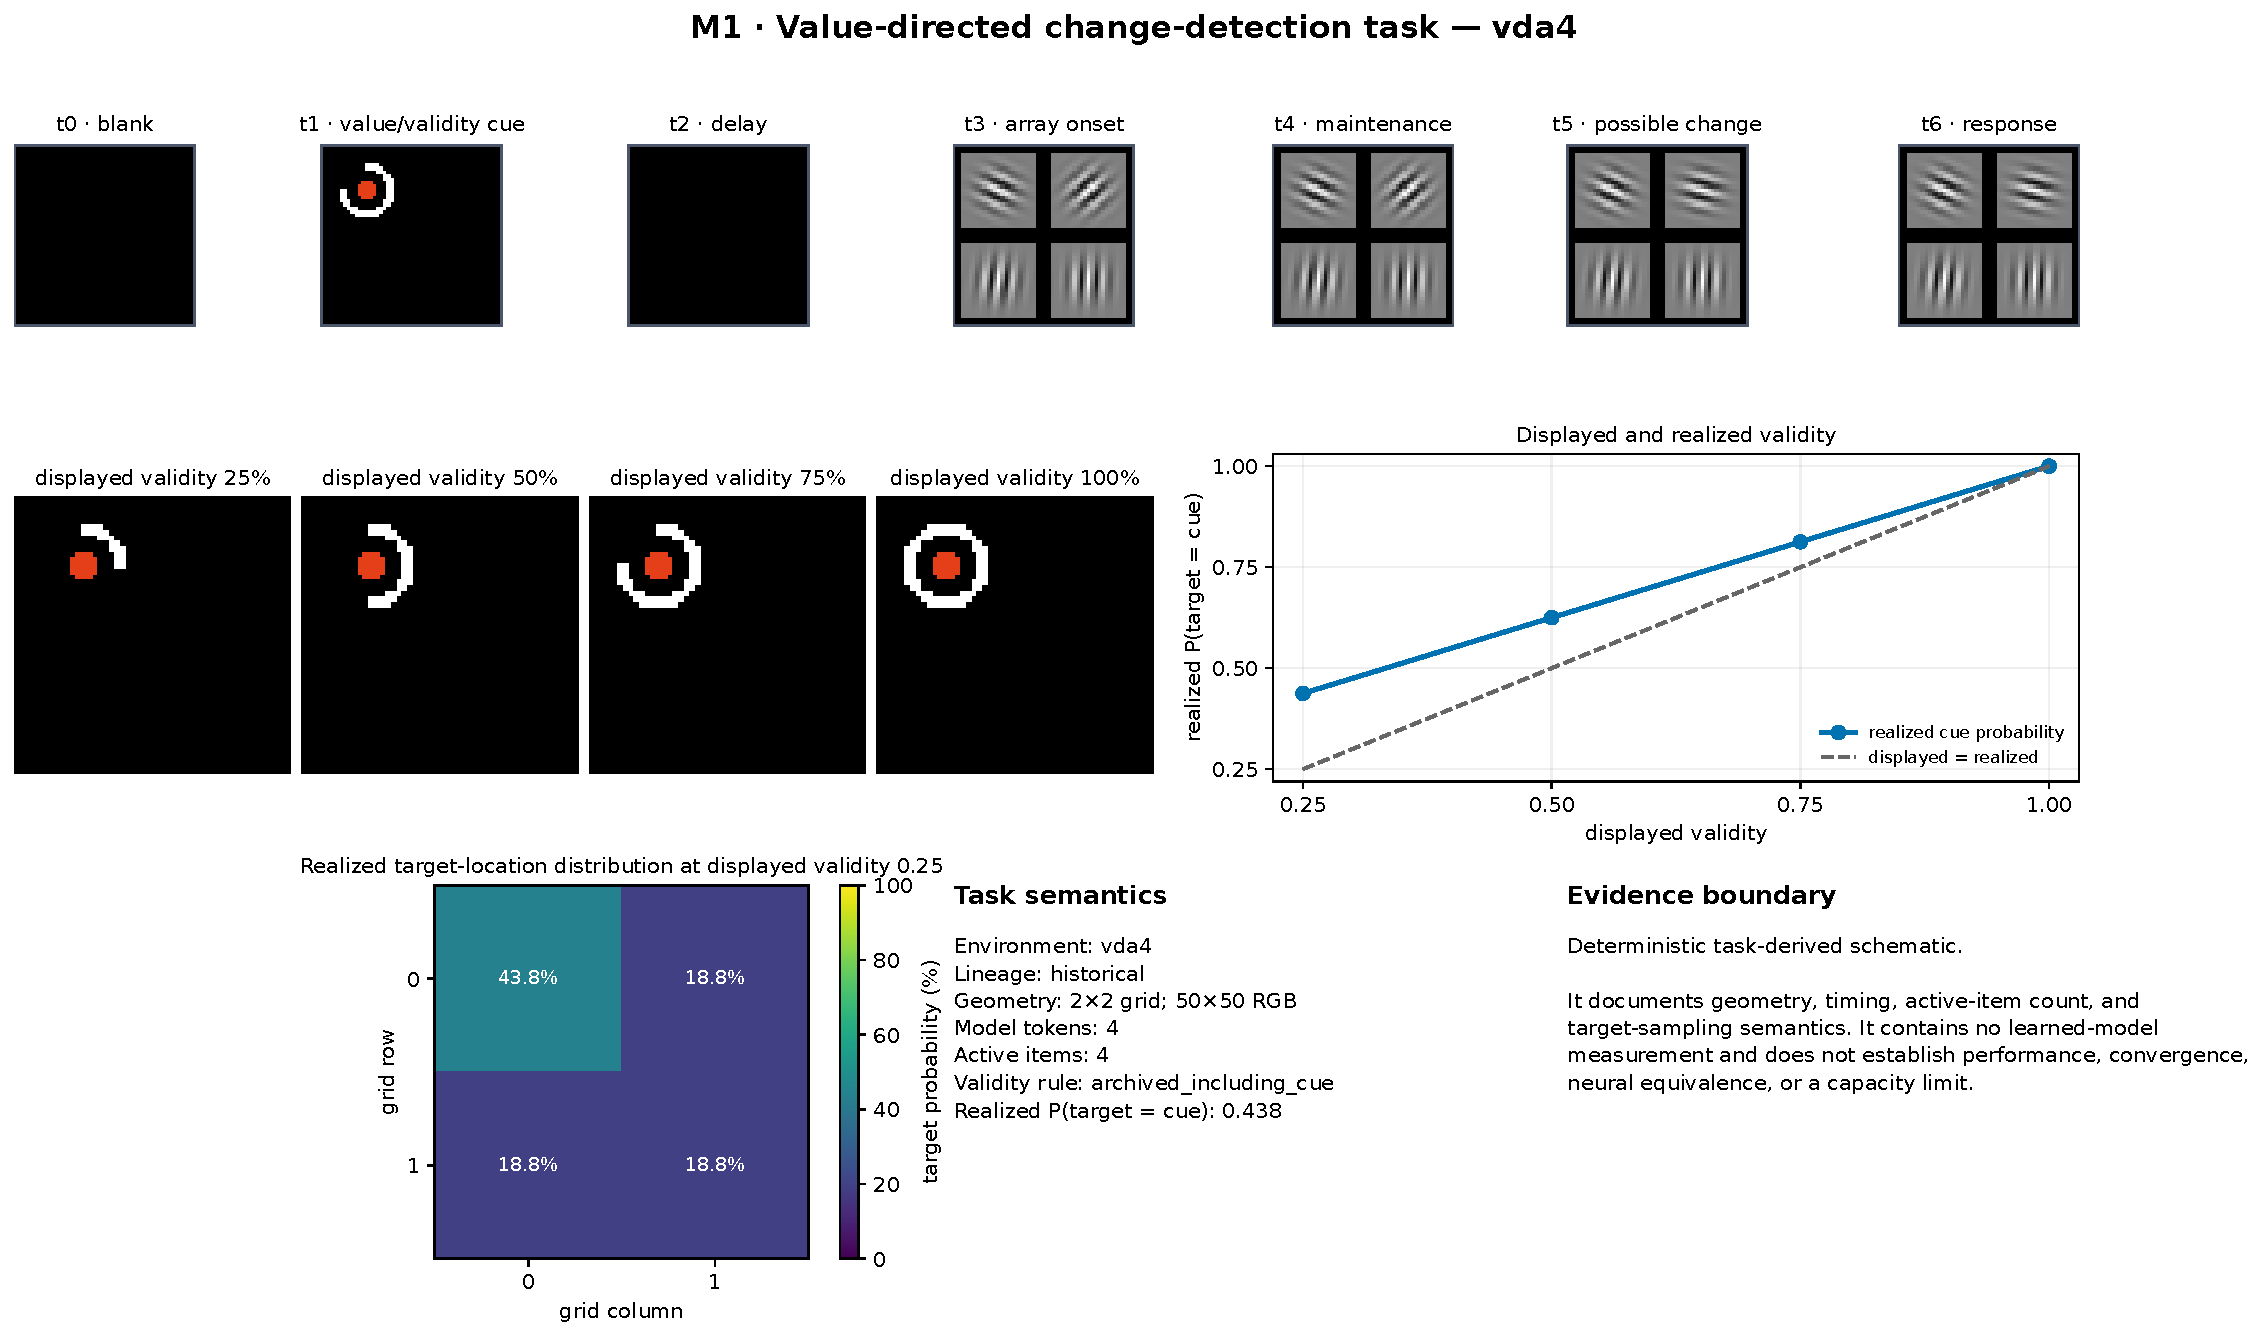
\includegraphics[width=0.97\linewidth]{m1_task_vda4.pdf}
\captionof{figure}{\textbf{Historical VDA4 task specification.} \eclass{Deterministic task-derived schematic.} The figure documents the seven-frame sequence, $2\times2$ geometry, four active items, four model tokens, and archived cue-including validity. At displayed validity 0.25, the realized cue probability is 0.438. It contains no learned-model measurement and establishes neither performance nor mechanism.}\label{fig:m1-historical}
\end{center}
\end{landscape}

\begin{landscape}
\thispagestyle{plain}
\begin{center}
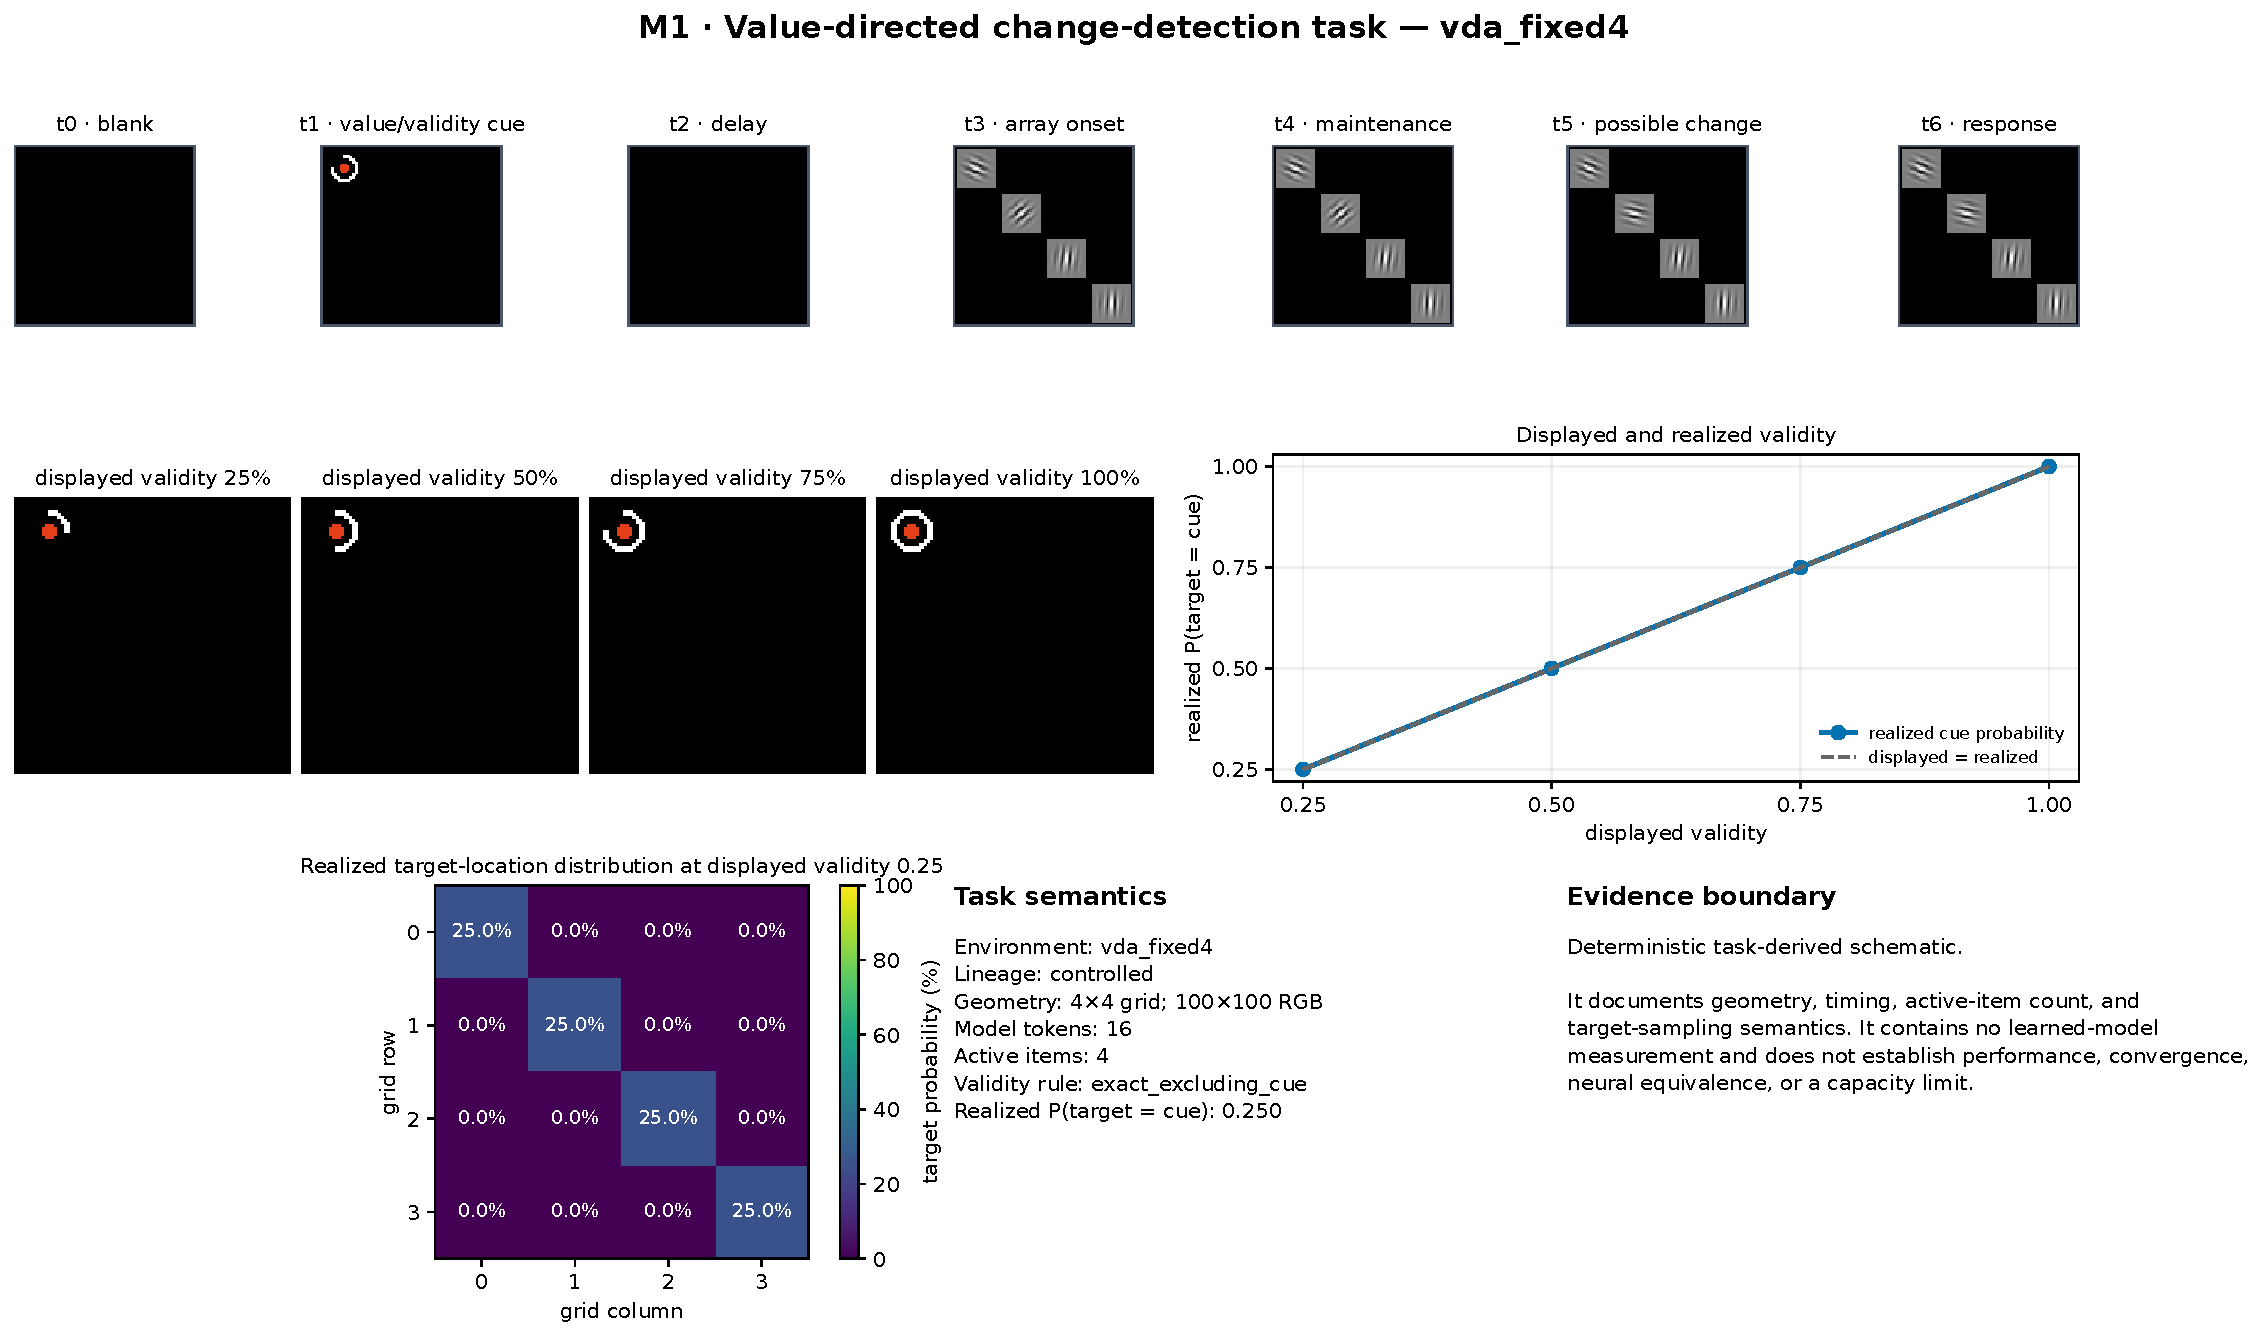
\includegraphics[width=0.97\linewidth]{m1_task_vda_fixed4.pdf}
\captionof{figure}{\textbf{Controlled fixed-grid VDA4 task specification.} \eclass{Deterministic task-derived schematic.} Across the controlled fixed-grid series, geometry is held at $4\times4$; unlike historical VDA4, this four-active-item task therefore has sixteen model tokens. Invalid targets exclude the cue, making displayed and realized validity equal. This is a protocol specification, not evidence that an accepted checkpoint exists.}\label{fig:m1-controlled}
\end{center}
\end{landscape}

\subsection{Architecture as specification, not result}
The architecture figures were generated from source-hashed specifications of \path{model.py}, \path{paper_encoder.py}, \path{paper_heads.py}, and \path{conv_frontend.py}. The shared pipeline preserves patch structure through routing and recurrent memory, then removes it at the actor/critic readout (Figure~\ref{fig:m2a}). In \env{affine\_ew}, memory produces element-wise scale and shift terms before self-attention (Figure~\ref{fig:m2b}). The spatial xLSTM updates a recurrent state independently at each patch position with shared parameters and feeds the next routing step (Figure~\ref{fig:m2c}). The \env{crossattn1} comparator instead queries with current visual tokens and concatenates visual and memory keys and values (Figure~\ref{fig:m2d}). These are implemented computational differences in the inspected current source. The M3 cache embeds neither code nor configuration hashes, so M2 does not prove that every historical cache label came from this exact source revision or run configuration. It is also not evidence that one route learned a better or more biologically faithful mechanism.

\captionof{table}{\textbf{Source-grounded architecture components.} Each row identifies the current-source anchor and the computational property audited from it; the table does not authenticate historical cache provenance.}\label{tab:architecture-components}
\begin{tabularx}{\textwidth}{@{}p{2.8cm}p{4.2cm}Y@{}}
\toprule
Component & Source anchor & Audited property\\
\midrule
Visual stem & \path{conv_frontend.py} & Converts the current RGB frame to a spatial token sequence; token count follows task geometry.\\
Affine router & \path{paper_encoder.py} & Applies memory-conditioned element-wise scale and shift before self-attention.\\
Cross-attention router & \path{paper_encoder.py} & Uses visual queries with visual and recurrent-memory keys and values.\\
Spatial recurrent state & \path{paper_encoder.py} & Updates xLSTM hidden and cell states independently by patch position with shared weights.\\
Policy/value readout & \path{paper_heads.py} & Flattens recurrent patch state for the two-action actor and quantile-regression critic.\\
Auxiliary predictor & \path{model.py} & Can add a training-only JEPA objective when enabled with nonzero loss weight; it is not part of inference-time behavior.\\
\bottomrule
\end{tabularx}

\begin{landscape}\thispagestyle{plain}\begin{center}
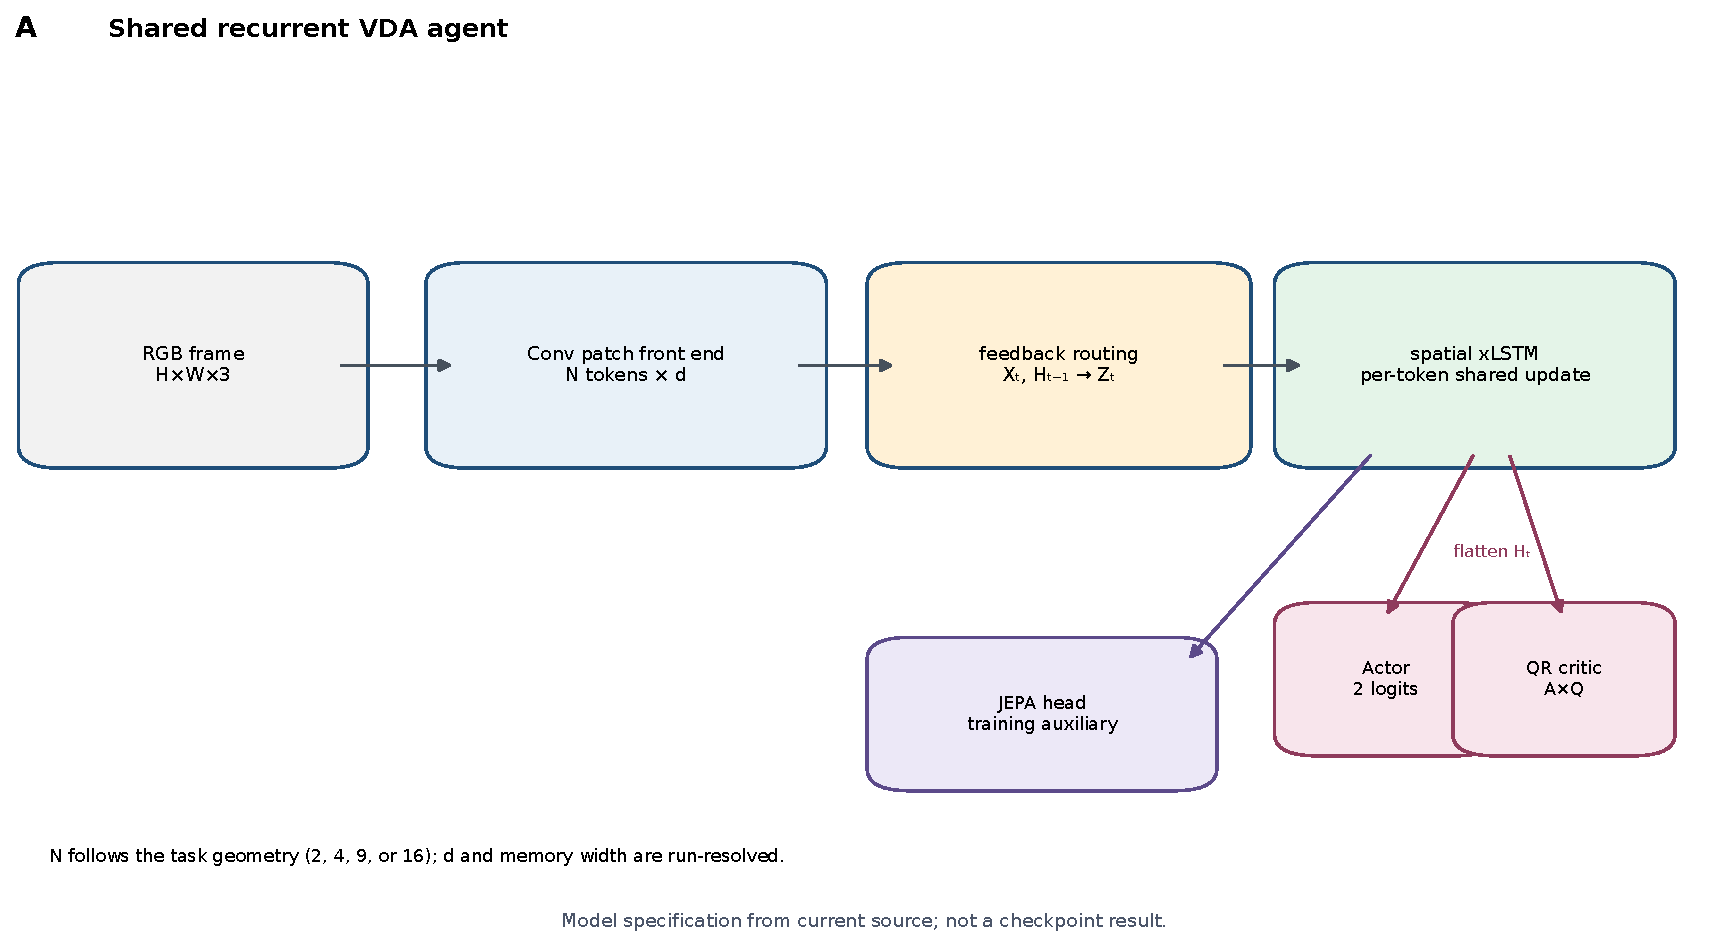
\includegraphics[width=0.97\linewidth]{m2_architecture_a.pdf}
\captionof{figure}{\textbf{M2A: shared recurrent agent.} \eclass{Source-derived model specification.} RGB frames become spatial patch tokens, undergo feedback routing, update a shared spatial xLSTM, and feed actor, quantile-regression critic, and an optional training-only JEPA readout. Token count follows task geometry; widths and JEPA enablement are run-resolved and are not established for historical cache entries.}\label{fig:m2a}
\end{center}\end{landscape}

\begin{landscape}\thispagestyle{plain}\begin{center}
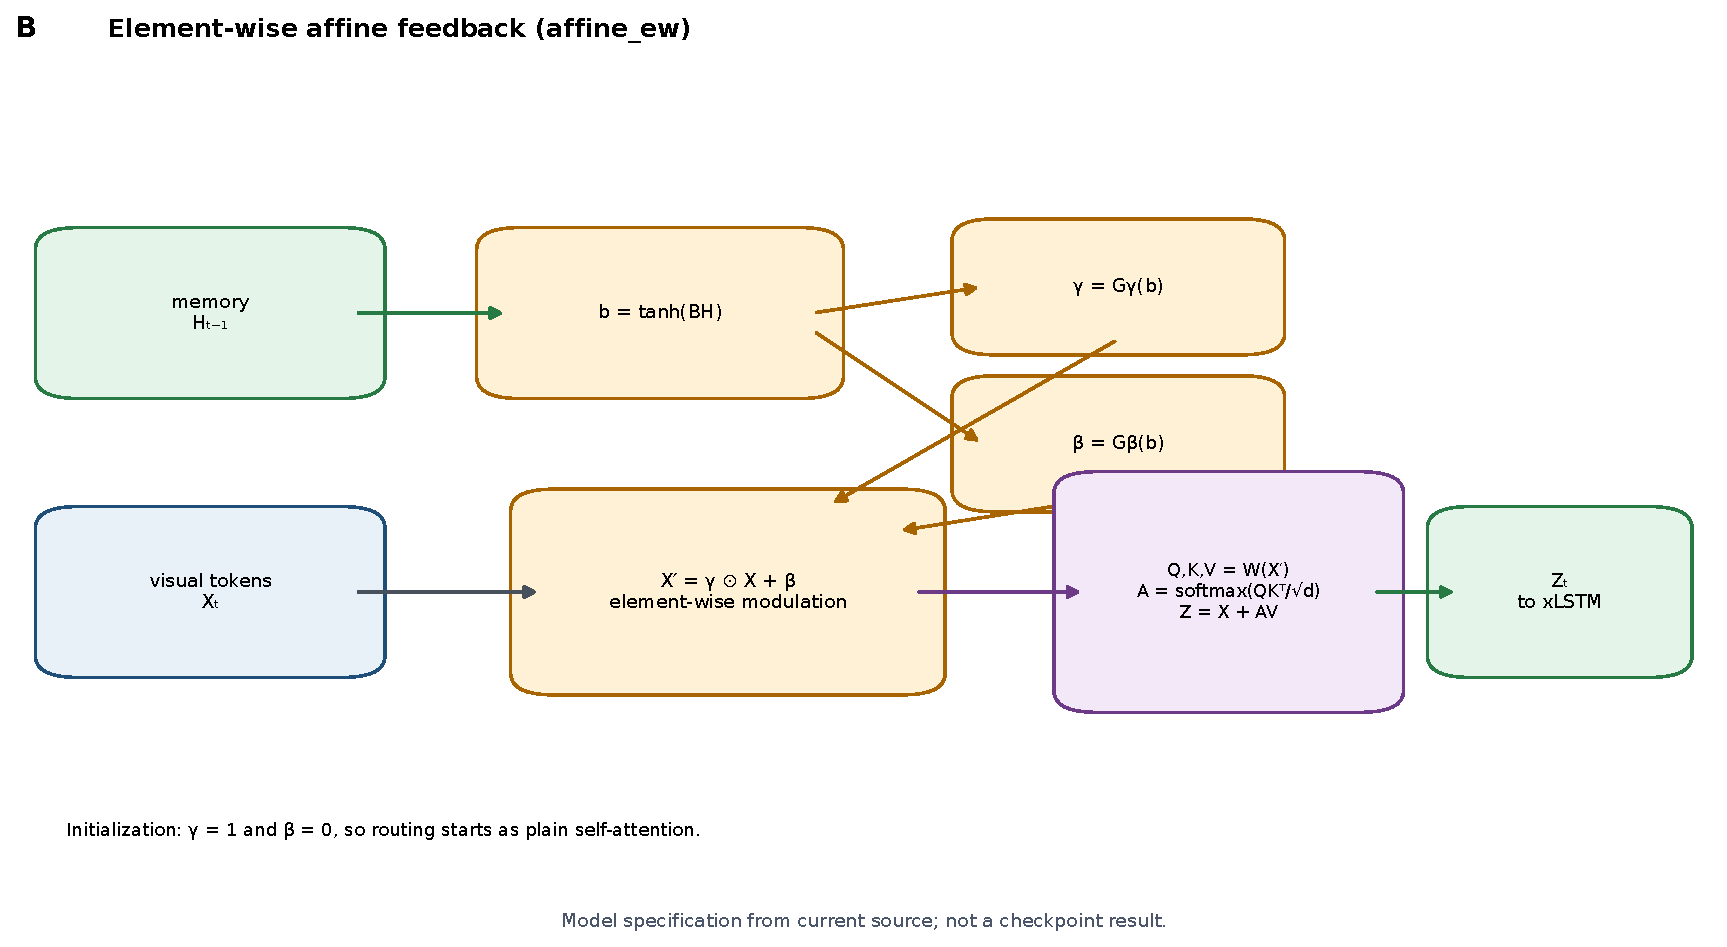
\includegraphics[width=0.97\linewidth]{m2_architecture_b.pdf}
\captionof{figure}{\textbf{M2B: element-wise affine feedback.} \eclass{Source-derived model specification.} Previous memory generates scale $\gamma$ and shift $\beta$, producing $X'=\gamma\odot X+\beta$ before self-attention. Identity initialization starts with $\gamma=1$ and $\beta=0$. The diagram does not show learned values.}\label{fig:m2b}
\end{center}\end{landscape}

\begin{landscape}\thispagestyle{plain}\begin{center}
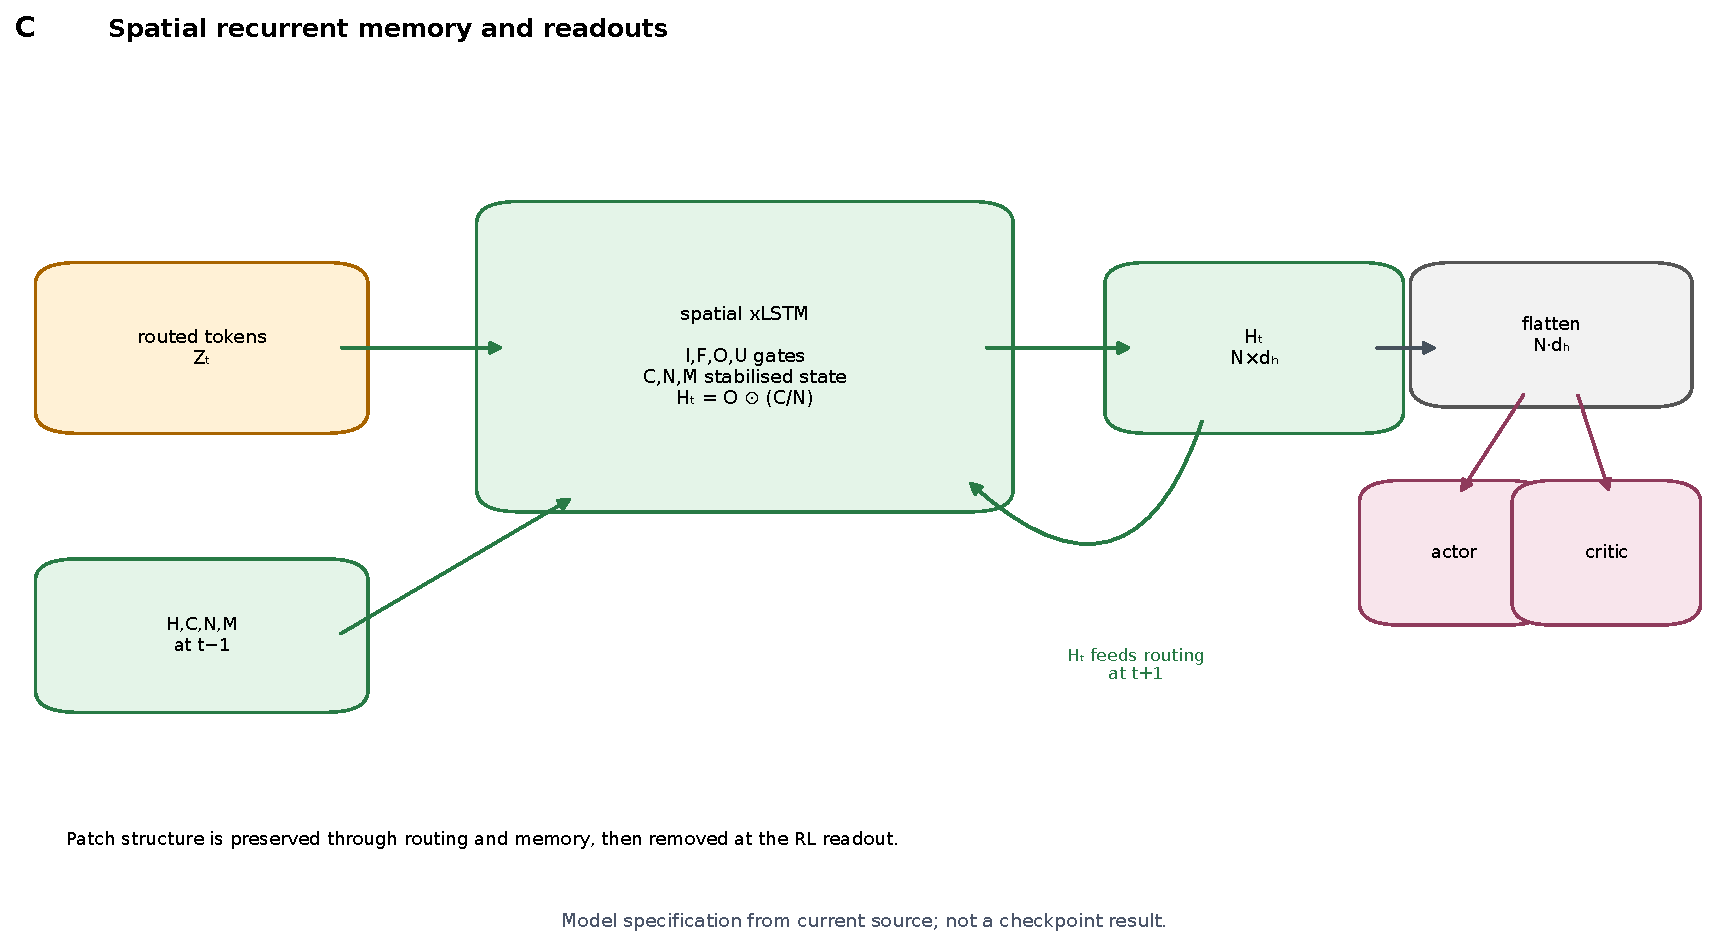
\includegraphics[width=0.97\linewidth]{m2_architecture_c.pdf}
\captionof{figure}{\textbf{M2C: spatial recurrent memory and readouts.} \eclass{Source-derived model specification.} Routed tokens and prior recurrent states enter the spatial xLSTM; the new hidden state both supplies the next routing step and, after flattening, feeds actor and critic. Arrow direction makes the temporal feedback boundary explicit.}\label{fig:m2c}
\end{center}\end{landscape}

\begin{landscape}\thispagestyle{plain}\begin{center}
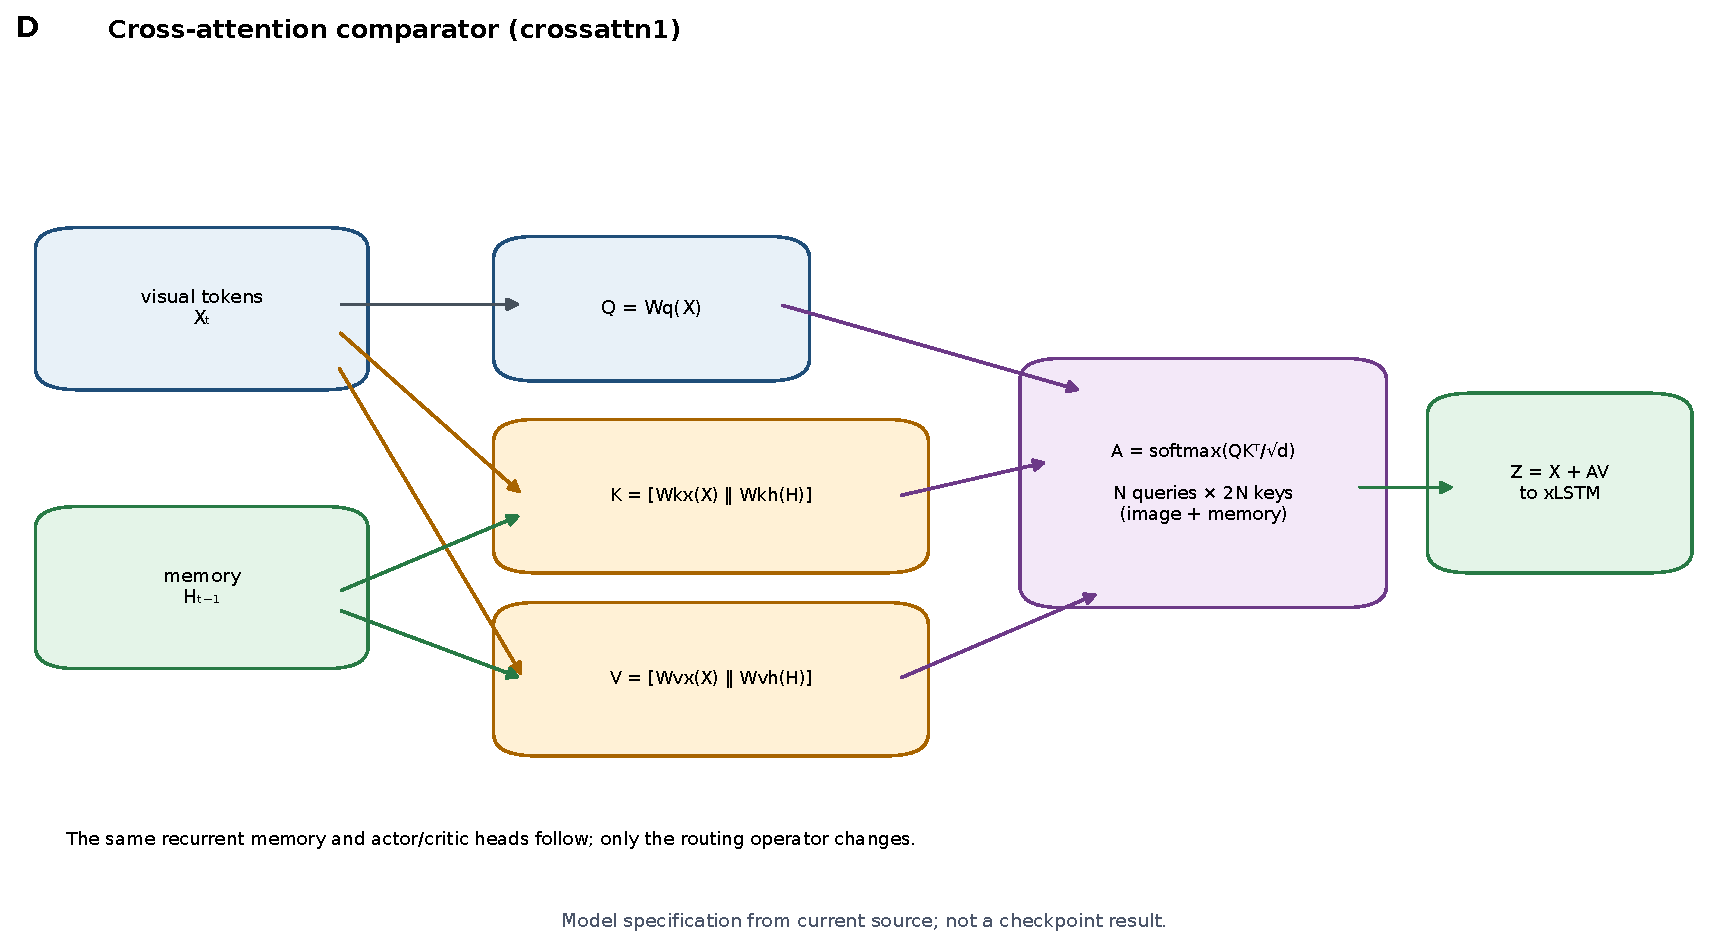
\includegraphics[width=0.97\linewidth]{m2_architecture_d.pdf}
\captionof{figure}{\textbf{M2D: cross-attention comparator.} \eclass{Source-derived model specification.} Current visual tokens provide queries while visual and recurrent-memory streams jointly provide keys and values. The same recurrent memory and policy heads follow; only the routing operator changes.}\label{fig:m2d}
\end{center}\end{landscape}

\section{Historical behavior regenerated from preserved aggregates}
\subsection{What was regenerated}
The admitted M3 figures read only the preserved \path{vda_sweep/figs/psych.npz} cache. The cache SHA-256 is recorded in every sidecar. Plotting does not import Torch or execute a checkpoint. Each figure displays cache arrays interpreted under the inspected current producer's location-conditioned score: change-response probability across all forced-location change trials and mean logical response frame among scored change responses, over ten orientation-change magnitudes and four displayed validity inputs. The current producer source states 300 trials per point, but the NPZ embeds neither its producer hash, checkpoint hash, per-point counts, nor evaluated uncued-location index. Task, routing-family, checkpoint-iteration, and producer-semantic identities are therefore cache-attributed rather than independently verified, and the spatial condition is called ``archived uncued'' rather than ``opposing.'' The archive contains aggregate point estimates only, so no sampling interval or seed-level variation can be reconstructed.

Across included cache entries, larger orientation changes are generally associated with higher change-response probability and a lower conditional mean response frame. Displayed-validity curves at the cued location are often close, while some VDA4 and VDA9 entries show descriptive cued--archived-uncued separation. Figure~\ref{fig:m3-overview} compares all eight entries; their full-resolution plates are retained in Appendix~\ref{app:m3-full}. Without intervals or seed-level estimates, apparent curve separations cannot establish precision or replication. Because the entries represent separately trained labels rather than a paired manipulation, they do not identify a within-model set-size effect, a routing effect, or a capacity limit.

\subsection{Singleton behavior: an explicit undefined estimand}
VDA1 has one active item. A cued change-response curve and conditional mean response-frame curve are defined; an uncued active comparator is not. Figures~\ref{fig:m3-vda1-affine} and \ref{fig:m3-vda1-cross} therefore retain panels B, C, E, and F as explicit ``Undefined'' panels rather than inventing a comparator.

\subsection{Two active items}
In VDA2, cued and archived uncued curves are both defined, although the NPZ does not prove the uncued spatial index. Their proximity in several panels is a descriptive property of cache entries labeled with that task and routing family. It is neither a precise null nor proof that recurrent memory is ``validity blind'': no interval, delay-specific cue decoder, forgetting analysis, or causal probe supports that conclusion.

\subsection{Four and nine active items}
Some VDA4 and VDA9 cache entries show descriptive differences between cued and archived uncued curves. This is cue-location-dependent behavior, not evidence of an internal allocation mechanism. Routing, memory, sensory encoding, fixed-location asymmetry, and response criterion remain possible explanations because geometry, token count, weights, and training history are not jointly controlled. A completed fixed-grid multi-seed series is the minimum matched design for estimating an active-item effect under the registered protocol; a capacity claim would additionally require a defined capacity estimand, accepted checkpoints, uncertainty, and evidence against training or readout failure.

\newcommand{\MThreeFullPlates}{%
\begin{landscape}\thispagestyle{plain}
\section{Full historical aggregate plates}\label{app:m3-full}
\begin{center}
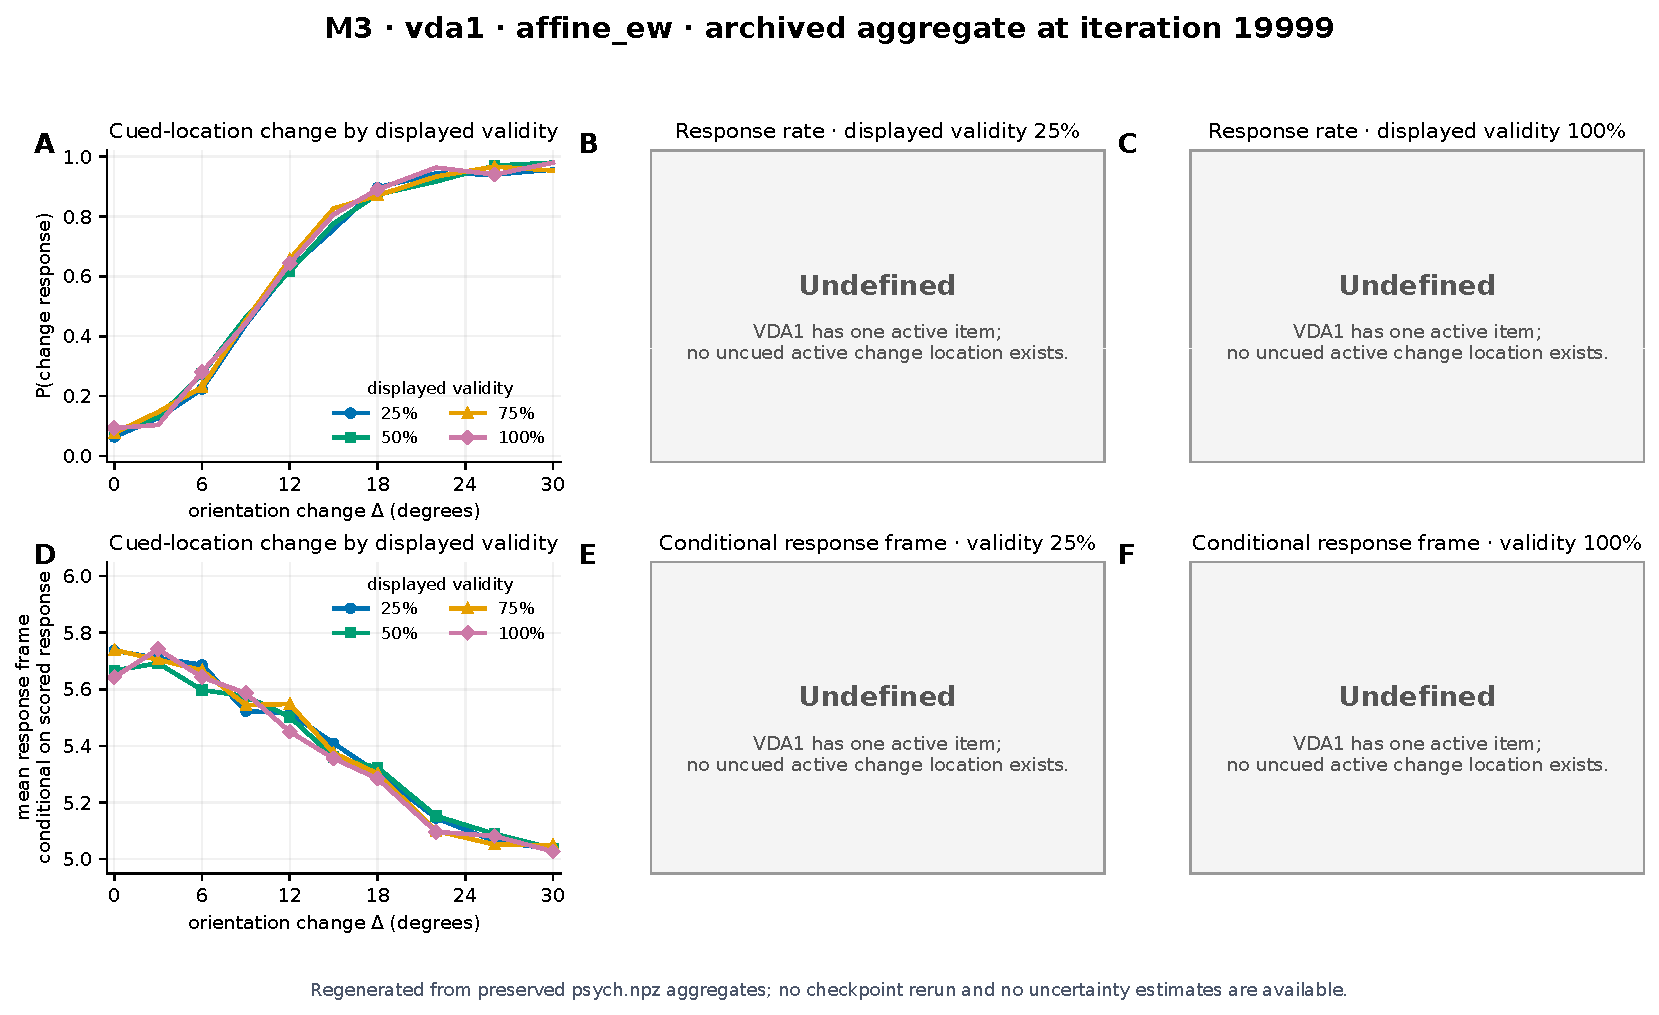
\includegraphics[width=0.89\linewidth]{m3_behavior_vda1_affine_ew.pdf}
\captionof{figure}{\textbf{Historical VDA1, affine feedback.} \eclass{Regenerated from preserved aggregate NPZ; checkpoint not rerun.} Change-response probability generally rises and conditional mean response frame falls with change magnitude. The singleton task defines only cued-location panels A and D; uncued-location panels B, C, E, and F are scientifically undefined. These are cache-attributed aggregate point estimates without reconstructable sampling intervals or training-seed replication.}\label{fig:m3-vda1-affine}
\end{center}\end{landscape}

\begin{landscape}\thispagestyle{plain}\begin{center}
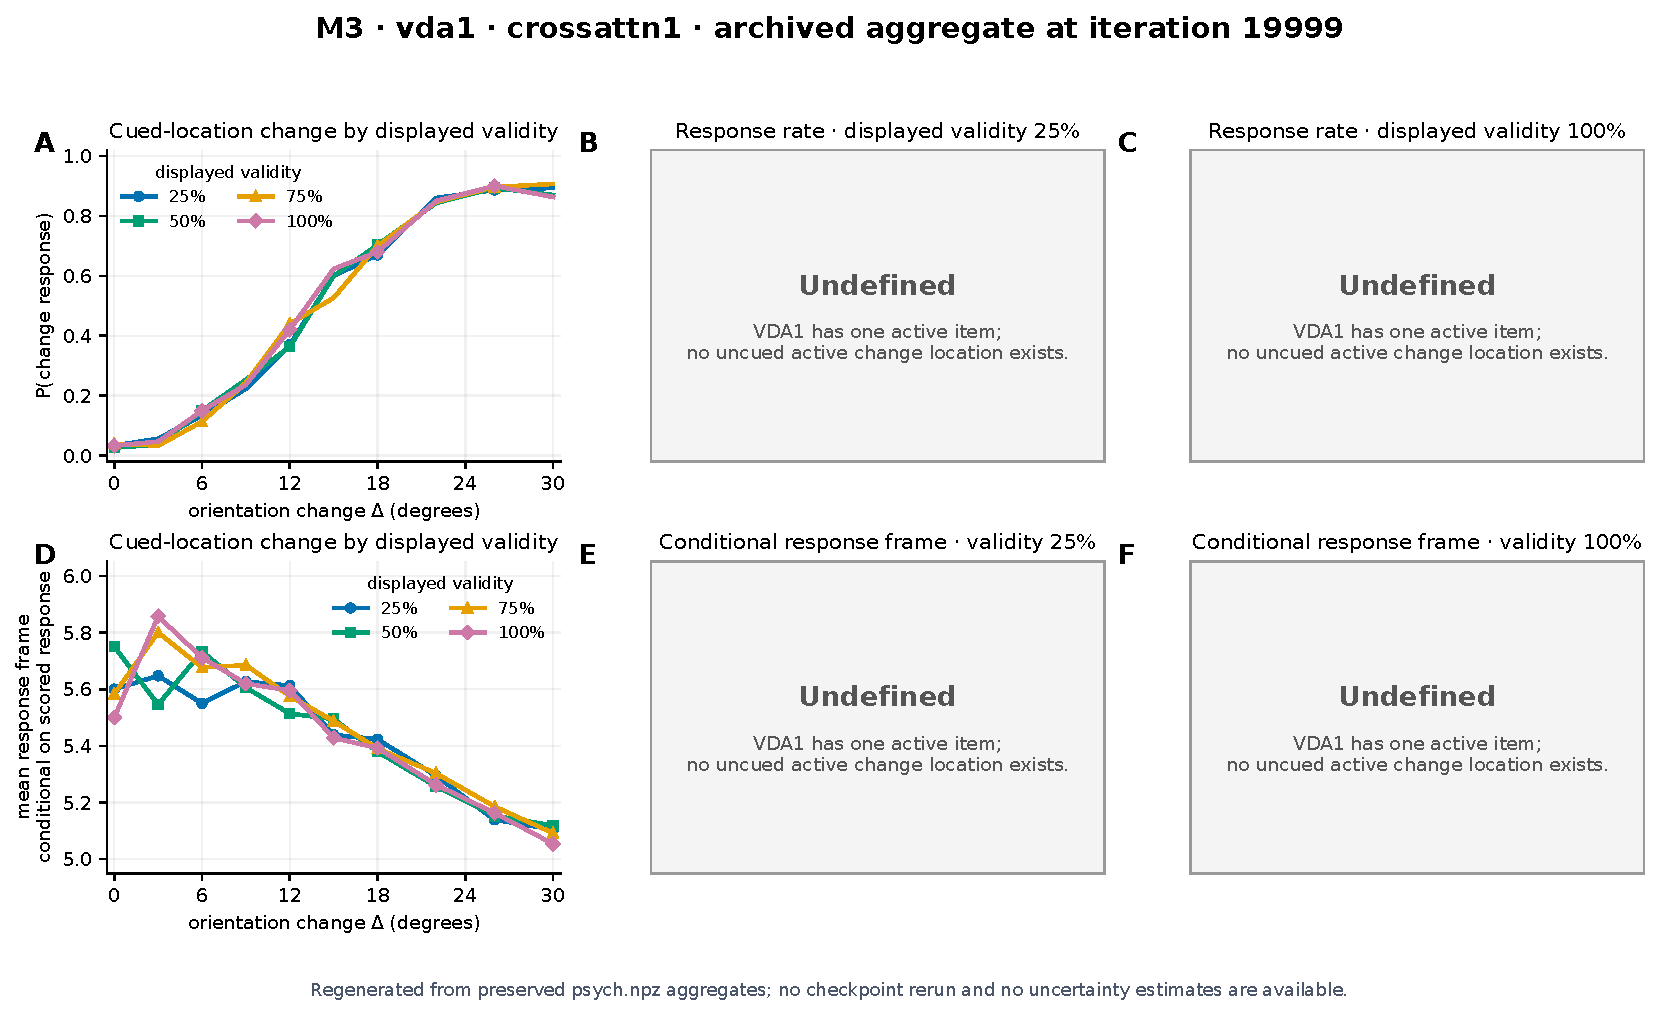
\includegraphics[width=0.89\linewidth]{m3_behavior_vda1_crossattn1.pdf}
\captionof{figure}{\textbf{Historical VDA1, cross-attention.} \eclass{Regenerated from preserved aggregate NPZ; checkpoint not rerun.} Change-response probability generally rises and conditional mean response frame falls with magnitude; no uncued active location exists. These are cache entries labeled VDA1/crossattn1, not an independently verified checkpoint execution, and they have no reconstructable interval or seed replication. They do not support an affine--cross-attention causal contrast.}\label{fig:m3-vda1-cross}
\end{center}\end{landscape}

\begin{landscape}\thispagestyle{plain}\begin{center}
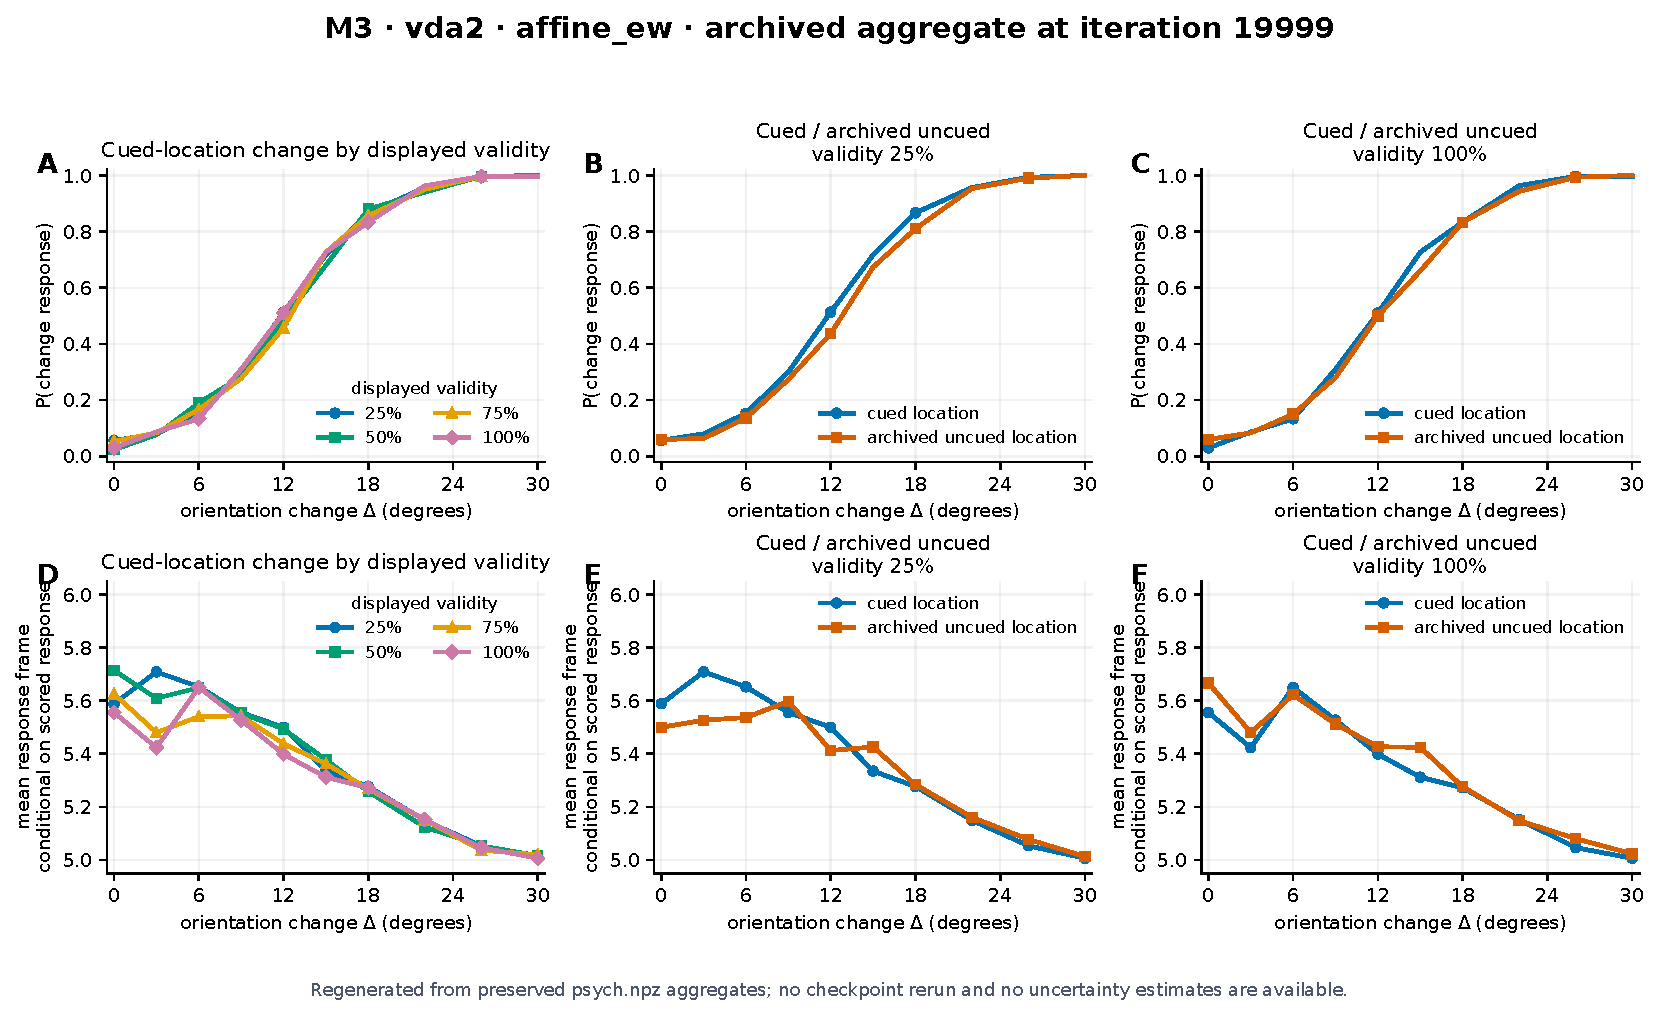
\includegraphics[width=0.89\linewidth]{m3_behavior_vda2_affine_ew.pdf}
\captionof{figure}{\textbf{Historical VDA2, affine feedback.} \eclass{Regenerated from preserved aggregate NPZ; checkpoint not rerun.} Cued and archived uncued curves are mostly close while response probability generally rises and conditional mean frame falls with magnitude. The NPZ does not prove the uncued spatial index. Aggregate point estimates without reconstructable intervals or seed replication cannot establish a precise null or routing contrast.}\label{fig:m3-vda2-affine}
\end{center}\end{landscape}

\begin{landscape}\thispagestyle{plain}\begin{center}
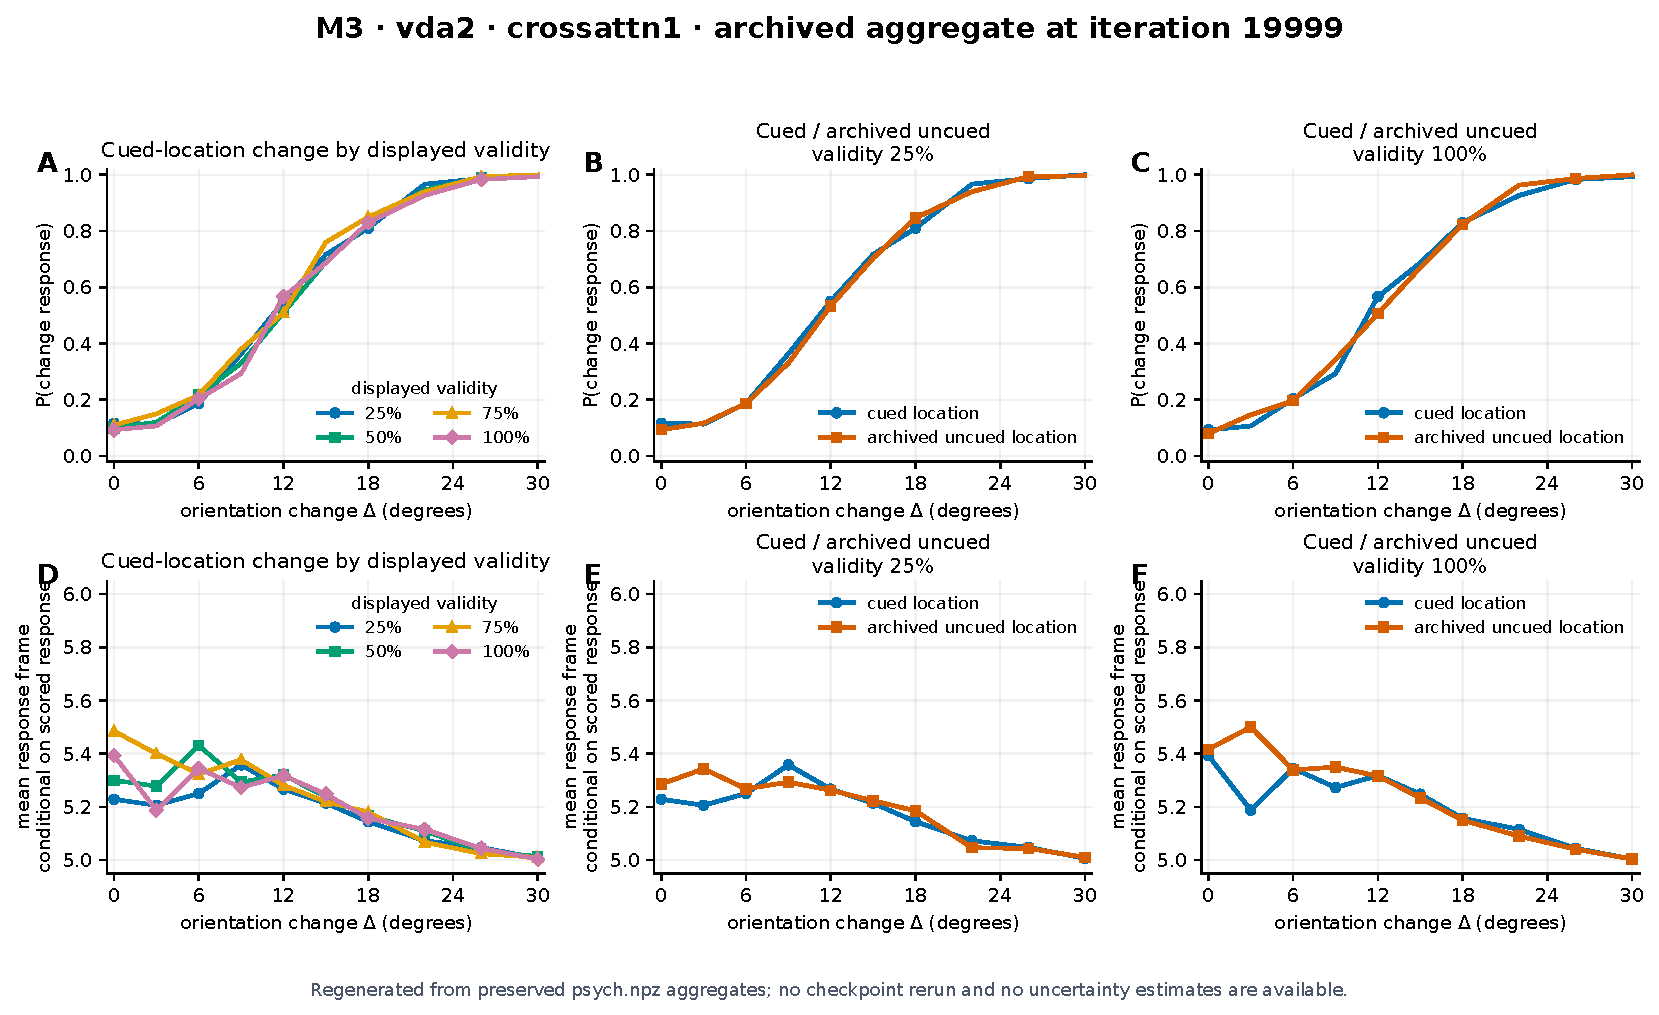
\includegraphics[width=0.89\linewidth]{m3_behavior_vda2_crossattn1.pdf}
\captionof{figure}{\textbf{Historical VDA2, cross-attention.} \eclass{Regenerated from preserved aggregate NPZ; checkpoint not rerun.} Cued and archived uncued point-estimate curves are mostly close, but the NPZ supplies neither their spatial index nor uncertainty or seed replication. Separate cache labels and training mean differences from Figure~\ref{fig:m3-vda2-affine} are descriptive associations, not a within-checkpoint routing intervention or a precise null.}\label{fig:m3-vda2-cross}
\end{center}\end{landscape}

\begin{landscape}\thispagestyle{plain}\begin{center}
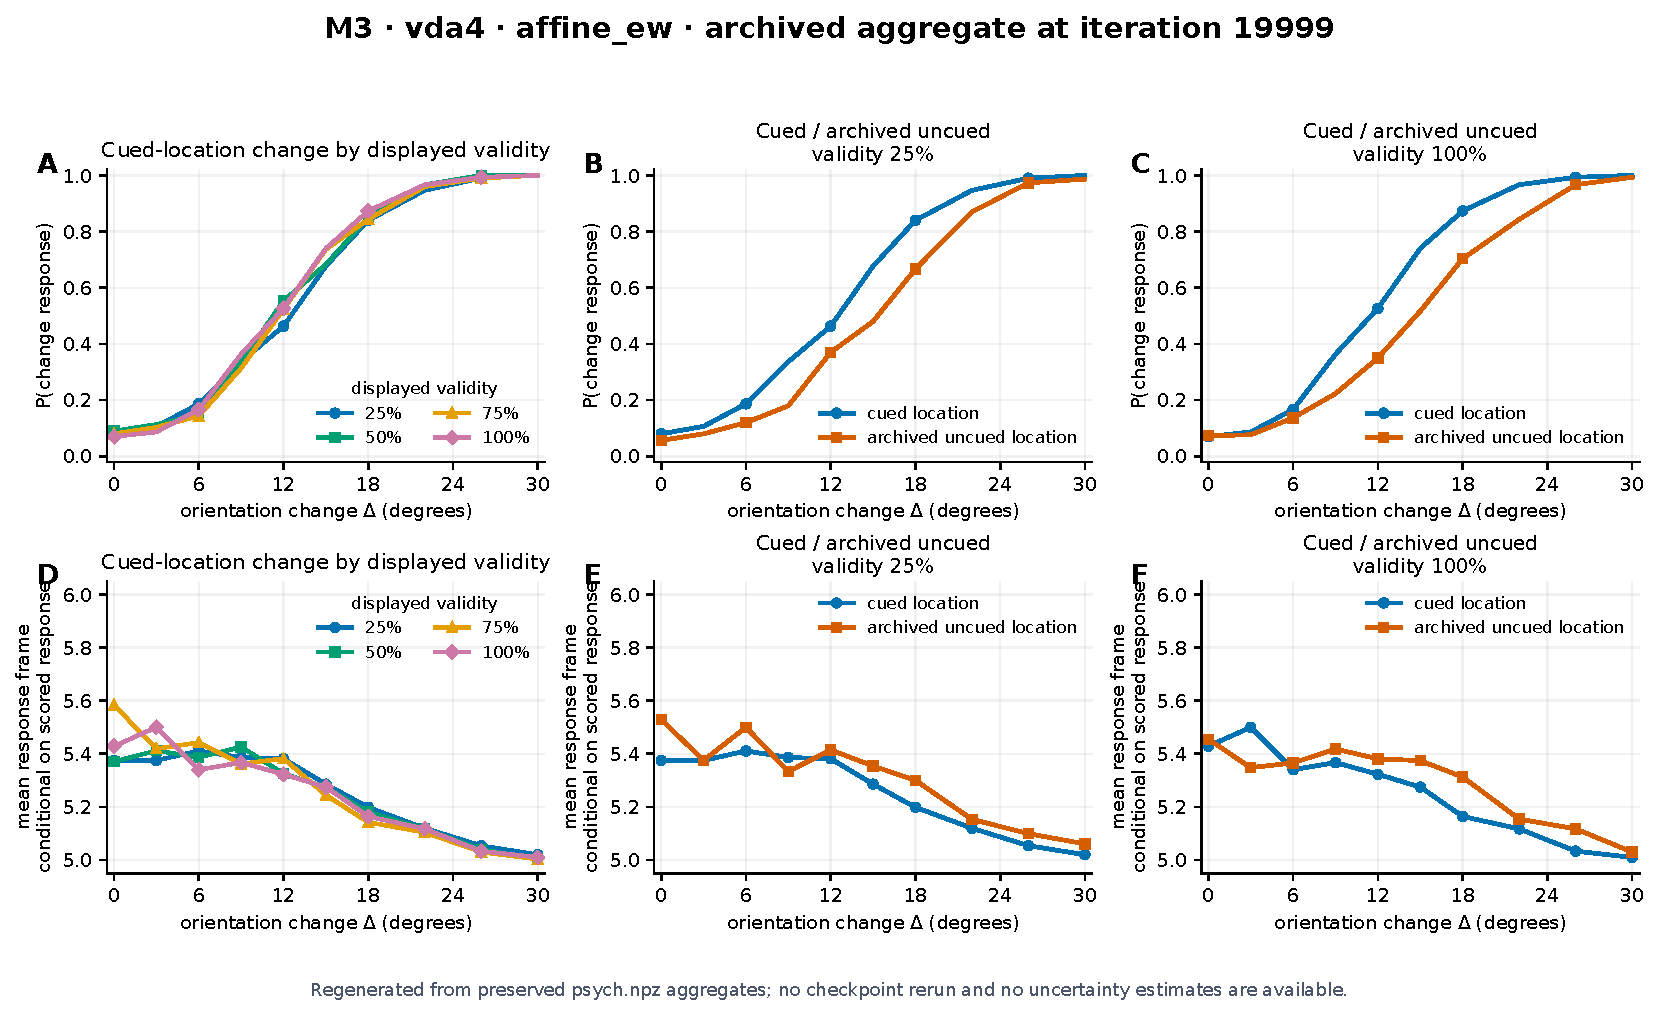
\includegraphics[width=0.89\linewidth]{m3_behavior_vda4_affine_ew.pdf}
\captionof{figure}{\textbf{Historical VDA4, affine feedback.} \eclass{Regenerated from preserved aggregate NPZ; checkpoint not rerun.} Cued and archived uncued curves show descriptive separation. The natural historical task realizes cue probability as $p+(1-p)/4$, but the inspected current producer forces change location within these curves rather than sampling that distribution. The NPZ does not prove the uncued spatial index, producer, or checkpoint identity; aggregate point estimates without intervals or seed replication do not establish allocation or a controlled effect.}\label{fig:m3-vda4-affine}
\end{center}\end{landscape}

\begin{landscape}\thispagestyle{plain}\begin{center}
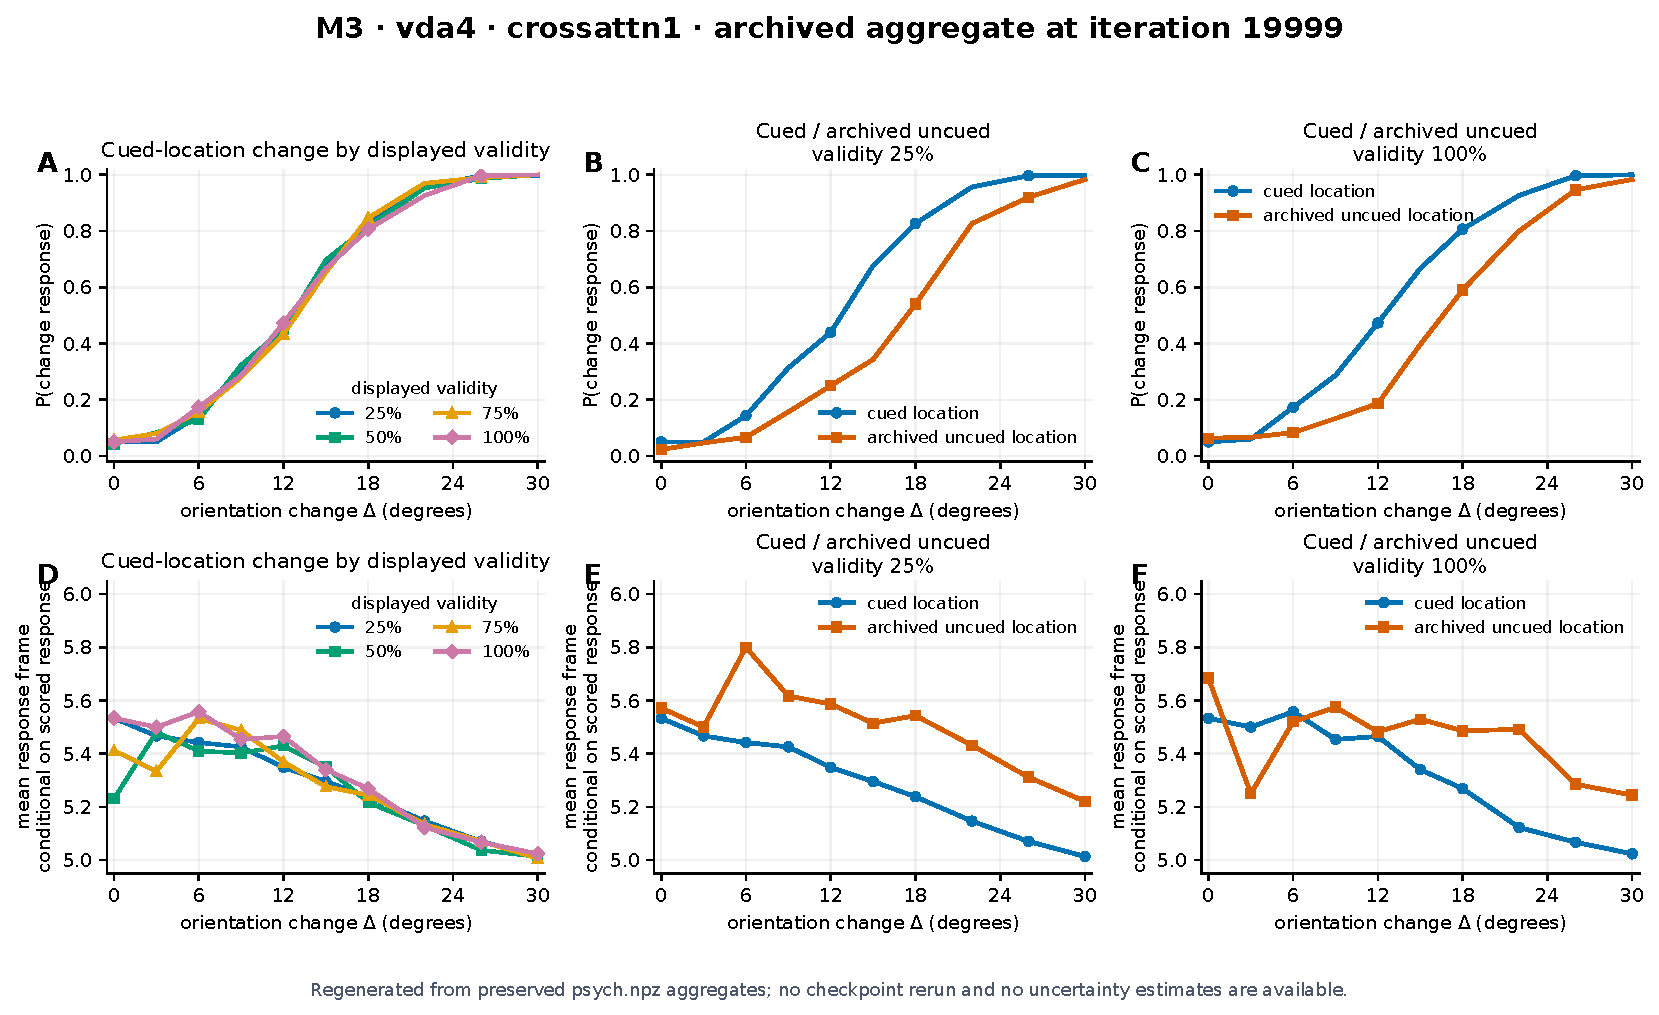
\includegraphics[width=0.89\linewidth]{m3_behavior_vda4_crossattn1.pdf}
\captionof{figure}{\textbf{Historical VDA4, cross-attention.} \eclass{Regenerated from preserved aggregate NPZ; checkpoint not rerun.} These displayed point estimates show pronounced cued--archived-uncued separation. The uncued index and checkpoint lineage are not cache-proven, and no reconstructable interval or seed replication establishes precision. This is not a matched-width within-model intervention on routing.}\label{fig:m3-vda4-cross}
\end{center}\end{landscape}

\begin{landscape}\thispagestyle{plain}\begin{center}
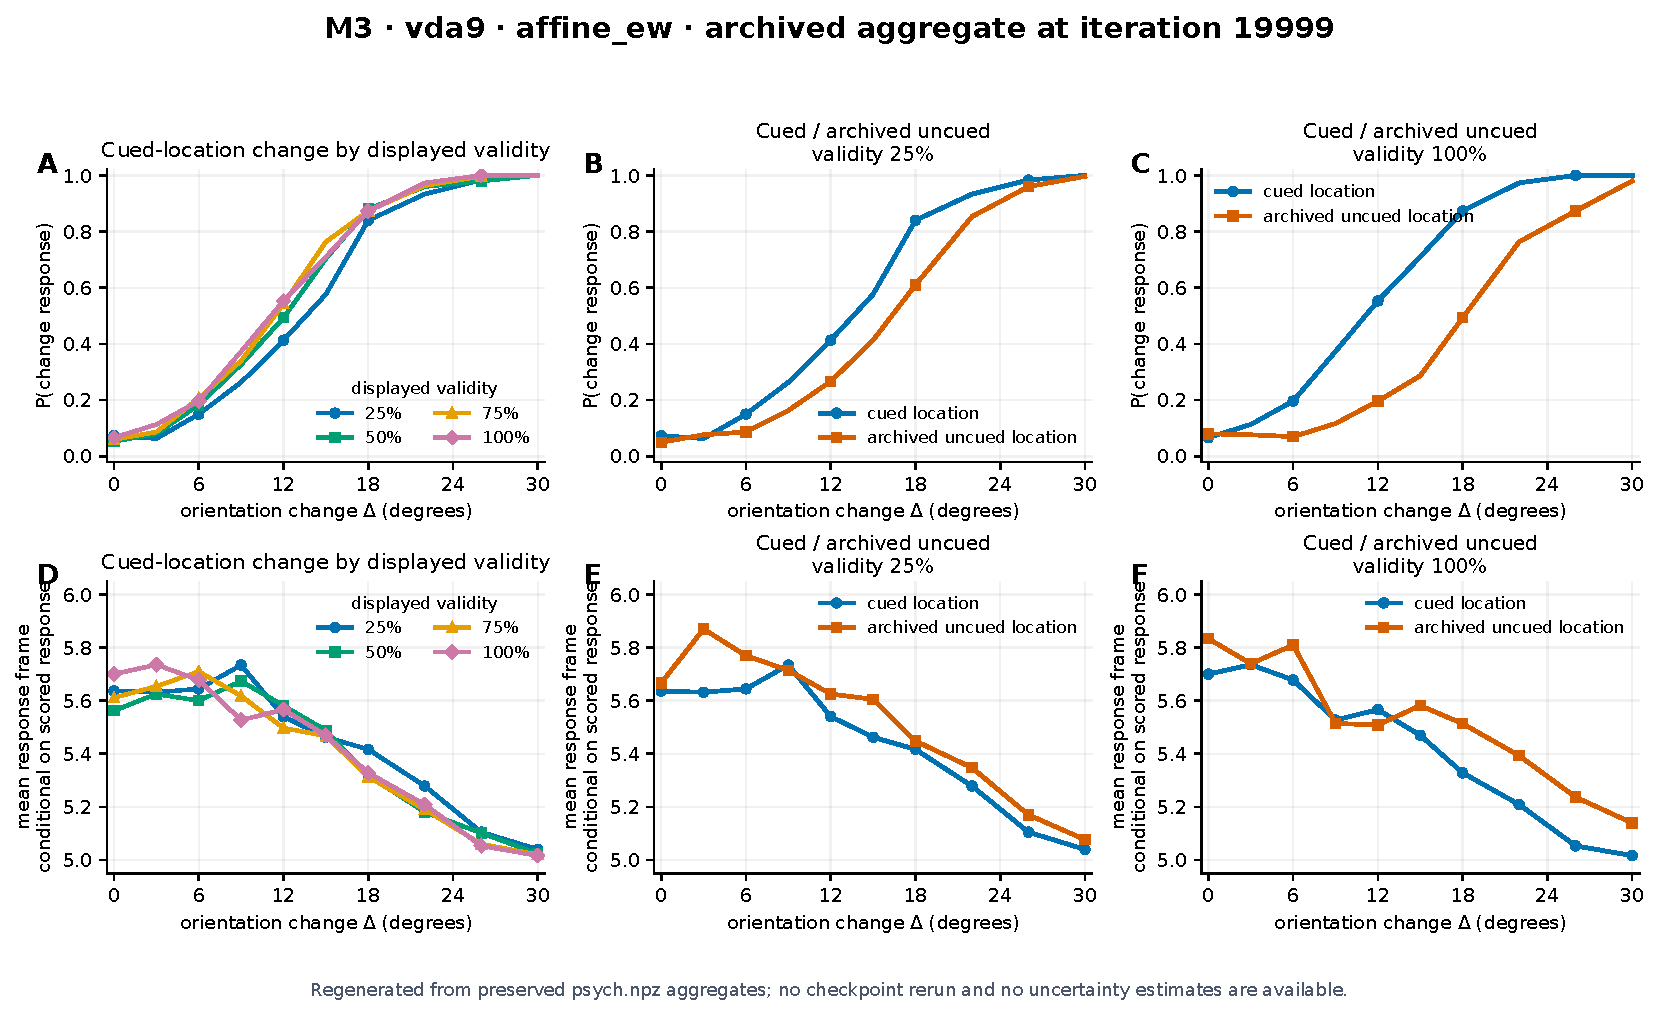
\includegraphics[width=0.89\linewidth]{m3_behavior_vda9_affine_ew.pdf}
\captionof{figure}{\textbf{Historical VDA9, affine feedback.} \eclass{Regenerated from preserved aggregate NPZ; checkpoint not rerun.} Cued and archived uncued point estimates differ. The natural historical task realizes cue probability as $p+(1-p)/9$, but the inspected current producer forces change location within these curves rather than sampling that distribution. The NPZ does not identify the uncued spatial index or independently verify checkpoint lineage, and absent intervals and seed replication preclude a precision, replication, or mechanism claim.}\label{fig:m3-vda9-affine}
\end{center}\end{landscape}

\begin{landscape}\thispagestyle{plain}\begin{center}
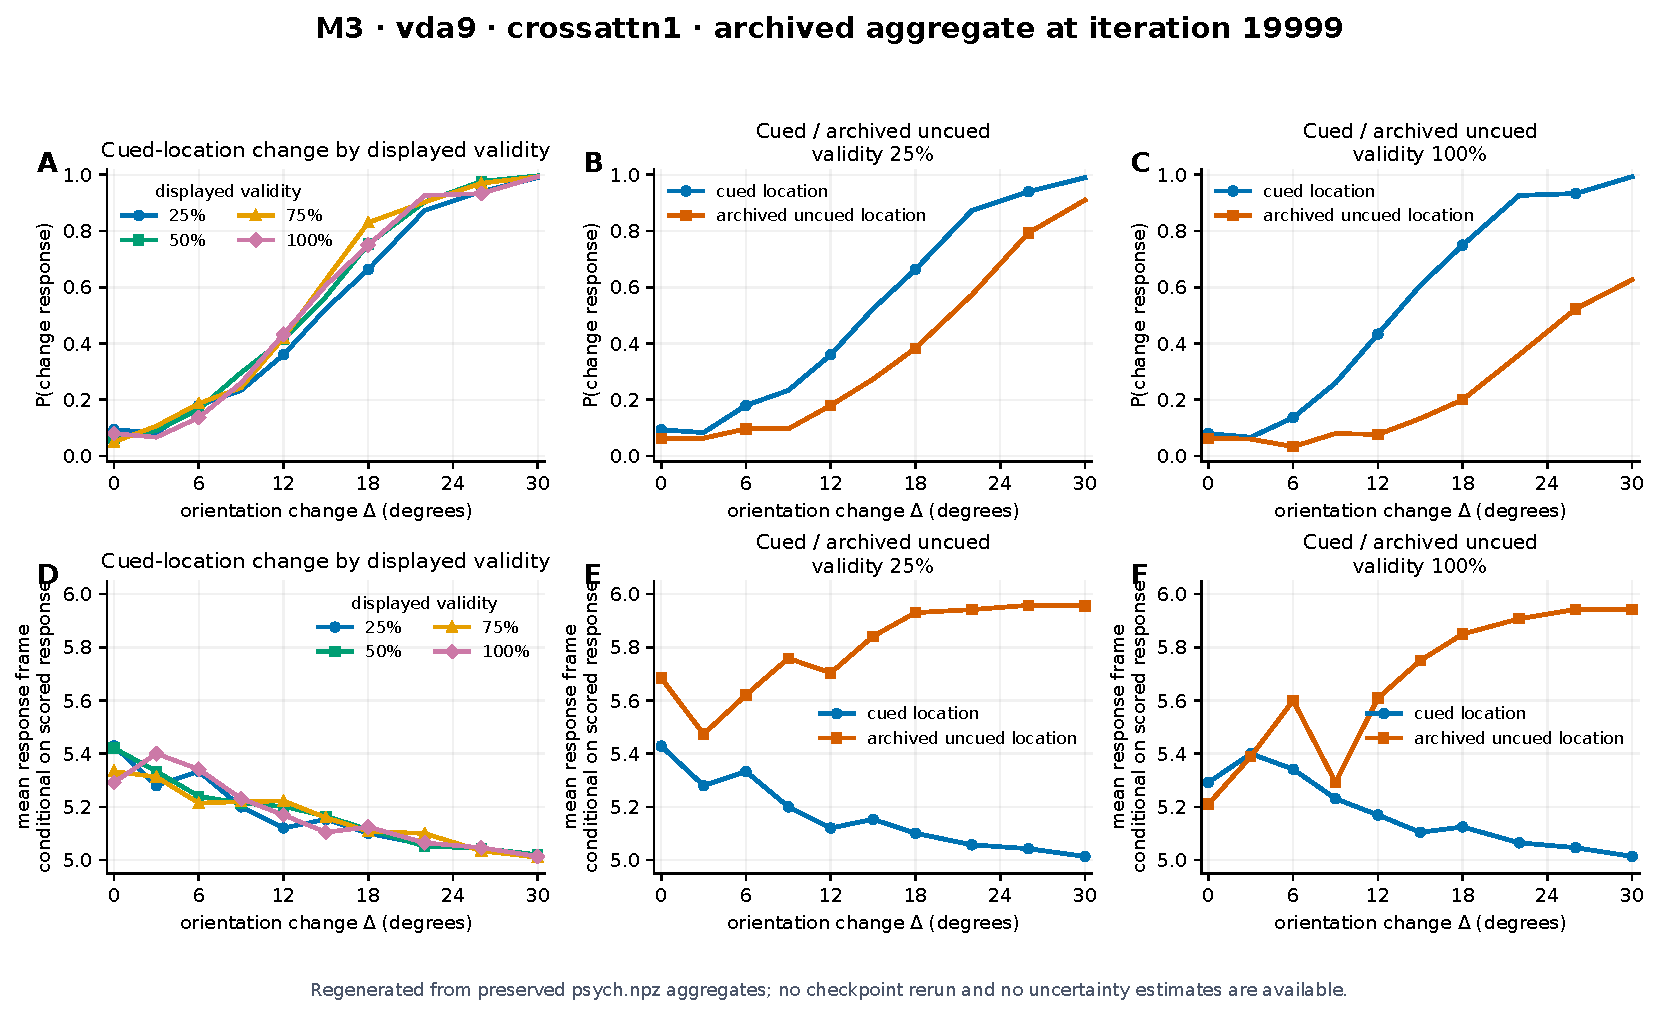
\includegraphics[width=0.89\linewidth]{m3_behavior_vda9_crossattn1.pdf}
\captionof{figure}{\textbf{Historical VDA9, cross-attention.} \eclass{Regenerated from preserved aggregate NPZ; checkpoint not rerun.} These point estimates show pronounced descriptive cued--archived-uncued separation. The uncued spatial index and checkpoint lineage are not cache-proven; absent intervals and independent seeds prevent precision or replication claims. Geometry, token count, weights, and training also differ, so this is not a controlled capacity or architecture estimate.}\label{fig:m3-vda9-cross}
\end{center}\end{landscape}
}

\clearpage
\thispagestyle{plain}
\begin{center}
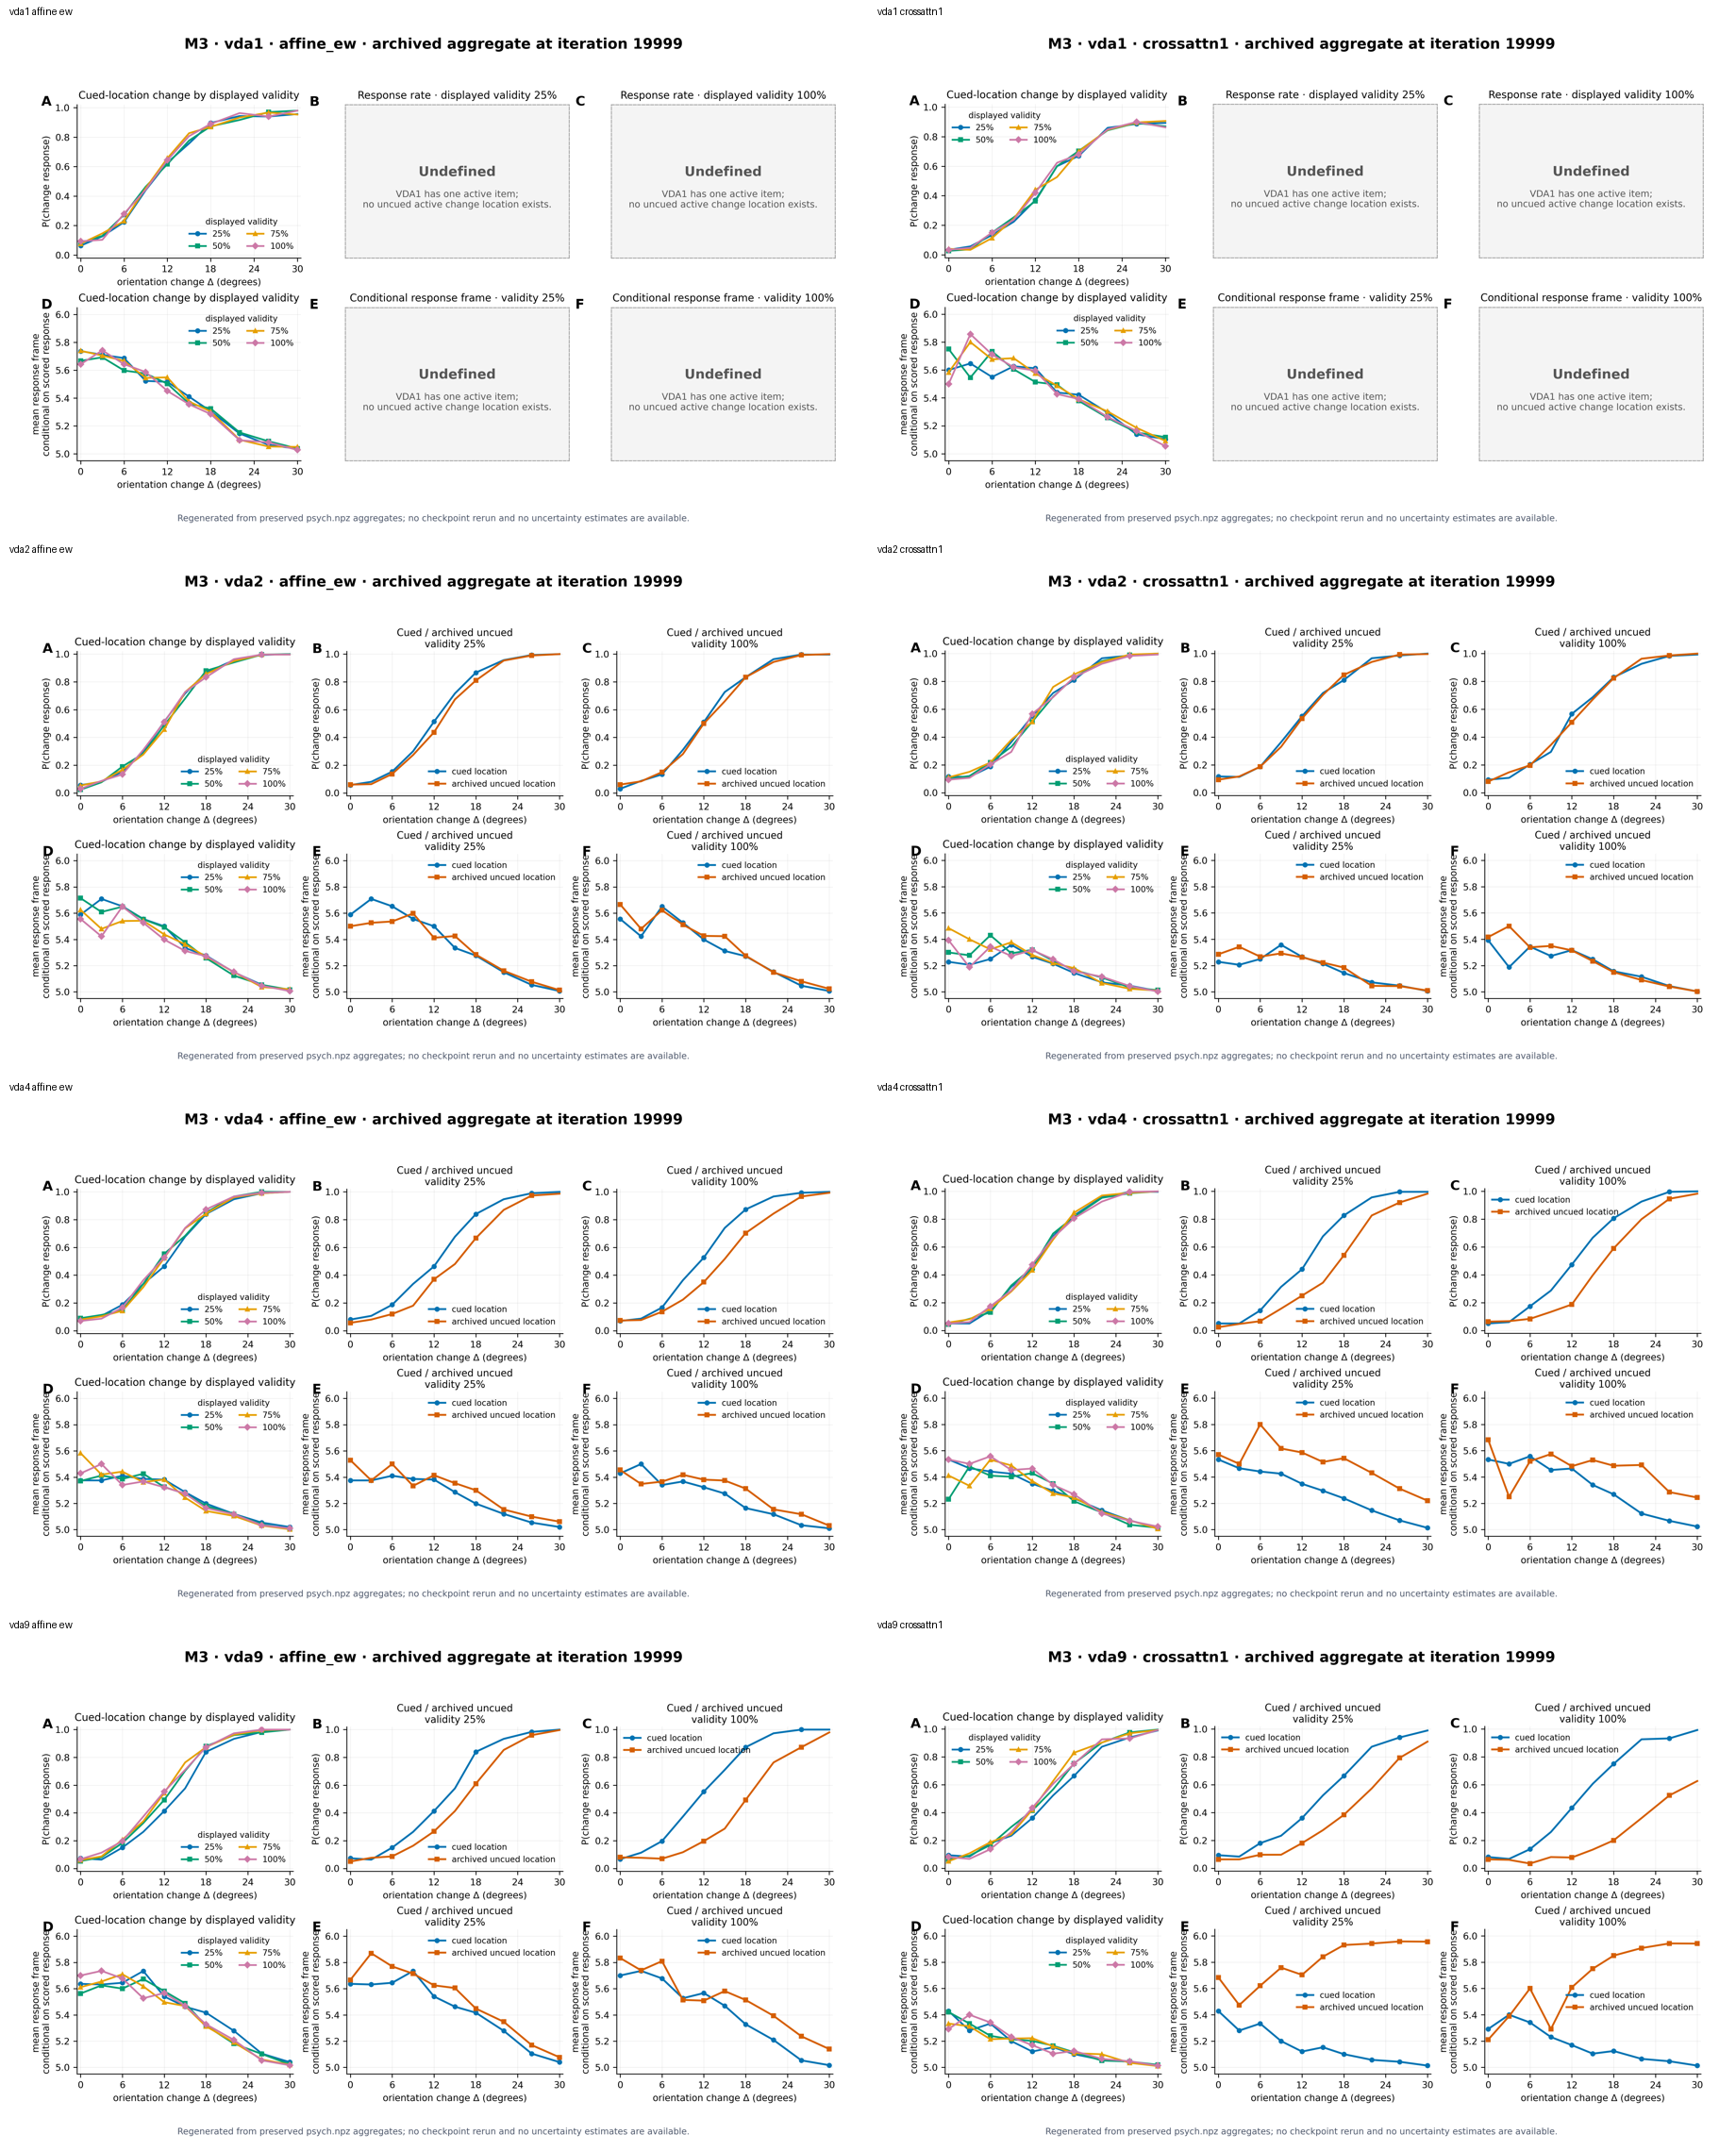
\includegraphics[width=0.96\linewidth]{m3_behavior_contact_sheet.png}
\captionof{figure}{\textbf{Comparative historical behavior overview.} \eclass{Regenerated from preserved aggregate NPZ; checkpoints not rerun.} Rows descend through VDA1, VDA2, VDA4, and VDA9; columns show affine then cross-attention routing. Within each plate, panels A--C show response probability and D--F conditional mean response frame; color encodes displayed validity in cued panels and spatial condition in cued-versus-archived-uncued panels. The overview preserves the three body-level scientific cases: VDA1 uncued estimands are undefined, VDA2 cued and archived-uncued curves are often close without establishing a precise null, and some VDA4/VDA9 entries show descriptive separation without identifying a mechanism or capacity law. Appendix~\ref{app:m3-full} contains the eight full-resolution plates and their evidence boundaries.}\label{fig:m3-overview}
\end{center}
\clearpage

\section{Checkpoint-recomputed first wave: VDA4 and VDA9}
\subsection{A distinct, provenance-closed evidence class}
The first wave does not retroactively validate the aggregate M3 cache. It is a separate recomputation from one independently selected iteration-19999 checkpoint for each task--routing label: historical VDA4 and VDA9 crossed with \env{affine\_ew} and \env{crossattn1}. Its immutable 77-file production tree binds executable source, dependencies, checkpoints, runtime, deterministic NPZ caches, and rendered products. The manifest SHA-256 is \texttt{c58a864a\ldots8c45706}; its read-only audit passed. Independent artifact review of the integrated candidate is recorded in the closure manifest.

All first-wave protocols fix the red cue at S1. The environment diagrams and valid psychometric condition place the change at S1, whereas the attention sweep omits physical changes entirely. The historical environments remain fully occupied: four locations in a $2\times2$ VDA4 grid and nine locations in a $3\times3$ VDA9 grid. For the psychometric location contrast, the bottom-right invalid comparator is therefore S4 for VDA4 and S9 for VDA9. Figures~\ref{fig:first-wave-env-vda4} and \ref{fig:first-wave-env-vda9} make that geometry explicit.

\begin{landscape}\thispagestyle{plain}\begin{center}
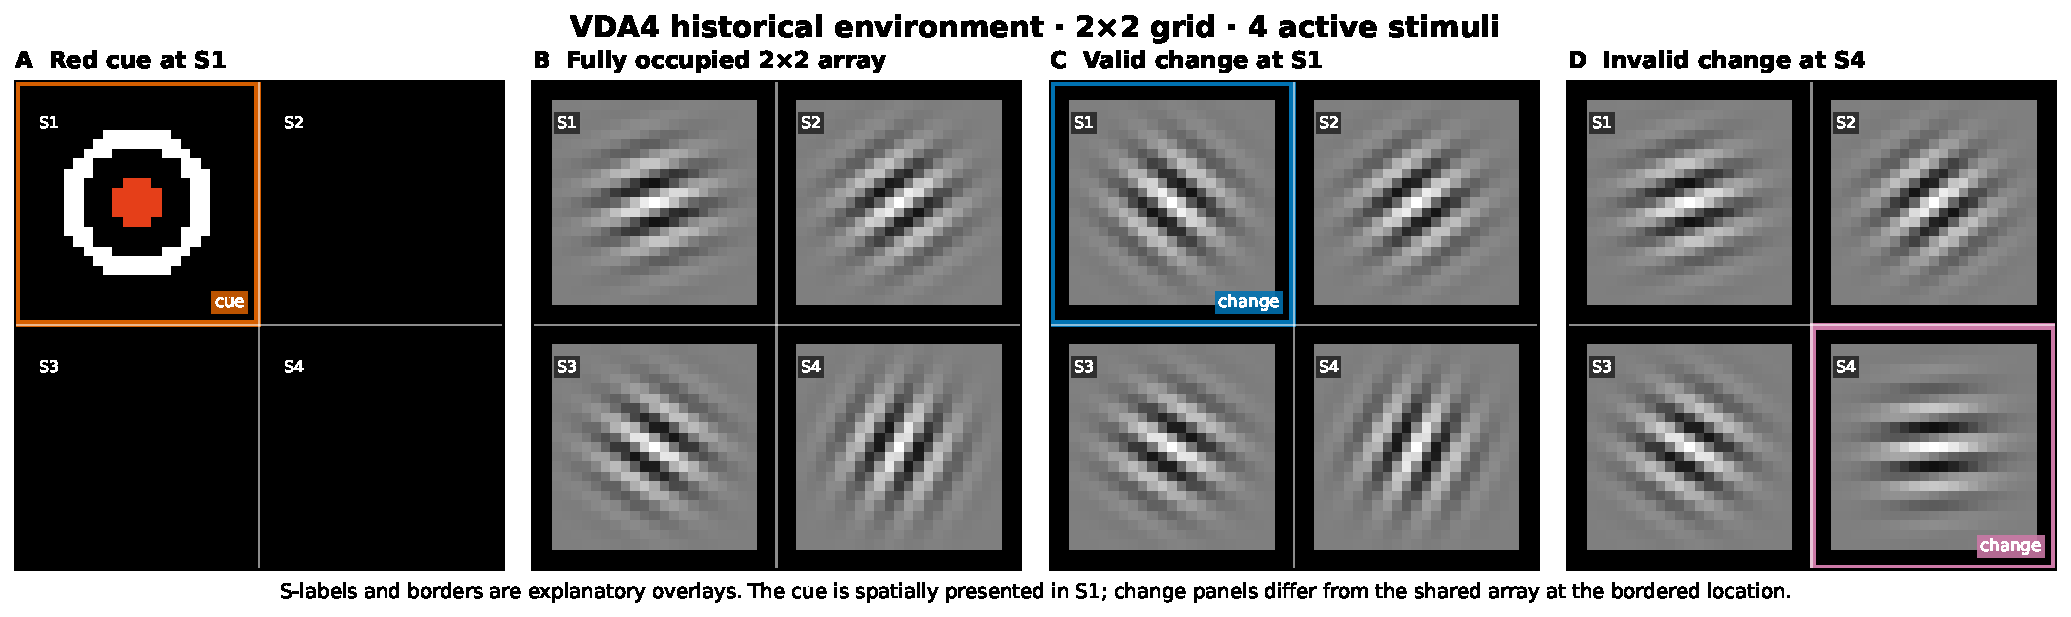
\includegraphics[width=0.90\linewidth]{first_wave_environment_vda4.pdf}
\captionof{figure}{\textbf{Verified historical VDA4 condition.} \eclass{Deterministic first-wave environment product.} The four occupied positions form the historical $2\times2$ geometry. S1 receives the red cue and the valid change; S4 is the registered bottom-right invalid location. Borders and S-labels are explanatory overlays rather than model measurements.}\label{fig:first-wave-env-vda4}
\vspace{0.6em}
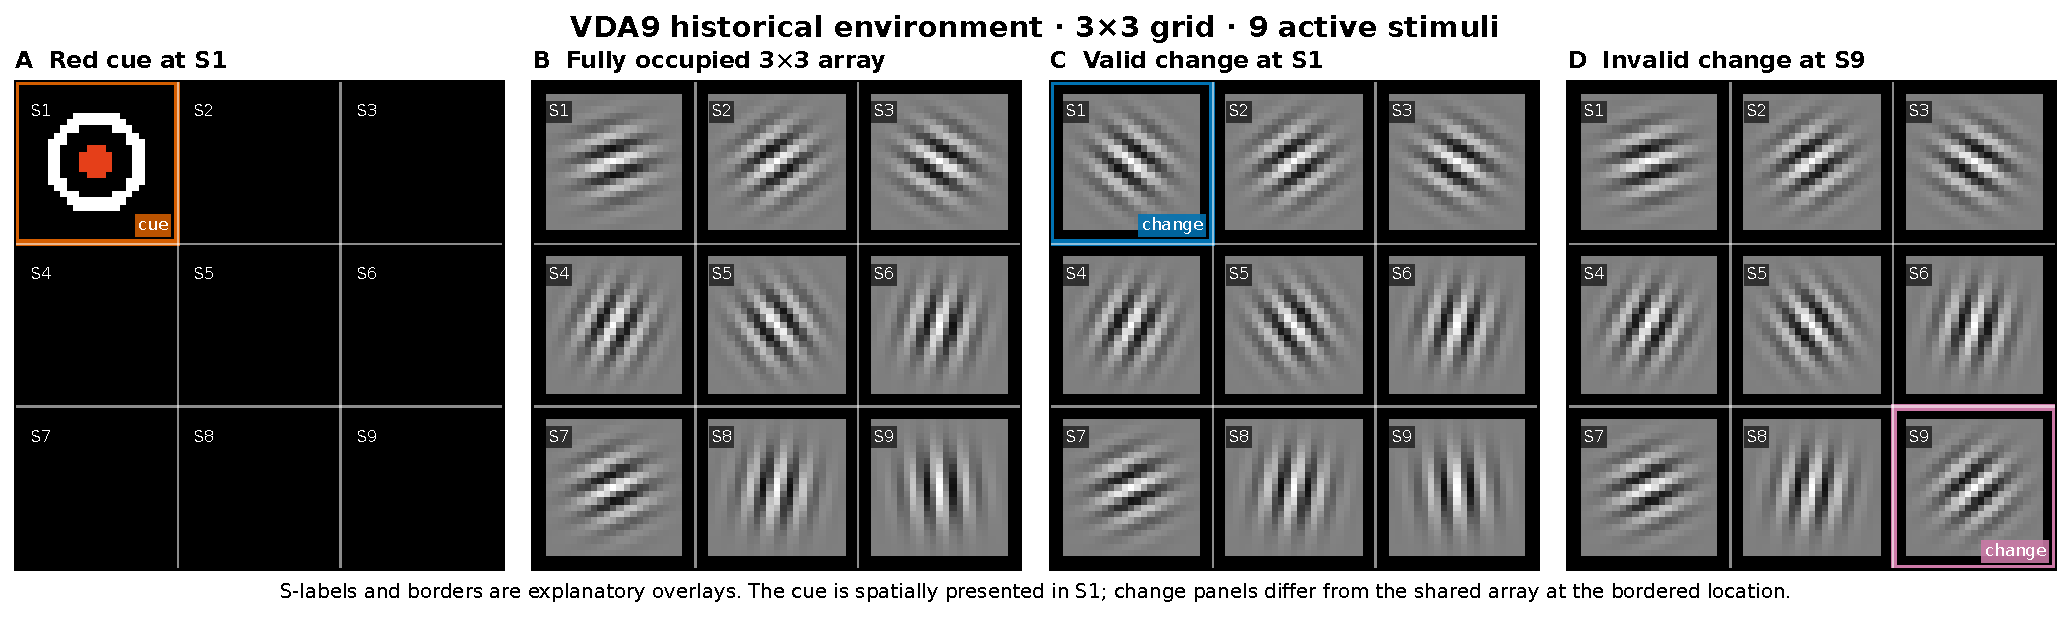
\includegraphics[width=0.90\linewidth]{first_wave_environment_vda9.pdf}
\captionof{figure}{\textbf{Verified historical VDA9 condition.} \eclass{Deterministic first-wave environment product.} The nine occupied positions form the historical $3\times3$ geometry. S1 receives the red cue and the valid change; S9 is the true bottom-right invalid location. This product is not the controlled fixed-grid task.}\label{fig:first-wave-env-vda9}
\end{center}\end{landscape}

\subsection{Event-aligned attention maps}
Each attention product evaluates four displayed cue proportions---25\%, 50\%, 75\%, and 100\%---using 96 matched deterministic trials per proportion. Every trial is a no-change trial: the cue remains fixed at S1, no orientation changes at any location, and t5 is retained only as the nominal change opportunity. Rows therefore encode cue proportion, while columns preserve logical timesteps t0--t6. Each cell averages all spatial query patches and displays the resulting attention mass over spatial keys. Affine attention has one spatial-key array. Cross-attention keeps image and recurrent-memory key groups separate as two cue-proportion-by-time arrays rather than summing them by location. A red outline marks the single fixed cue location. Each figure uses a shared scale from zero to its observed maximum; the scale is fixed within, but not across, figures.

These maps ask whether changing cue proportion modulates routing weights at the nominal change opportunity when no physical change occurs. Matched seeds hold the underlying no-change display realization constant across cue proportions within each trial index. The maps remain descriptive averages: they do not establish response causation, improved discriminability, persistent information content, or biological attention. Because no invalid-change attention contrast is included, M4C and M4D remain partial.

\begin{landscape}\thispagestyle{plain}\begin{center}
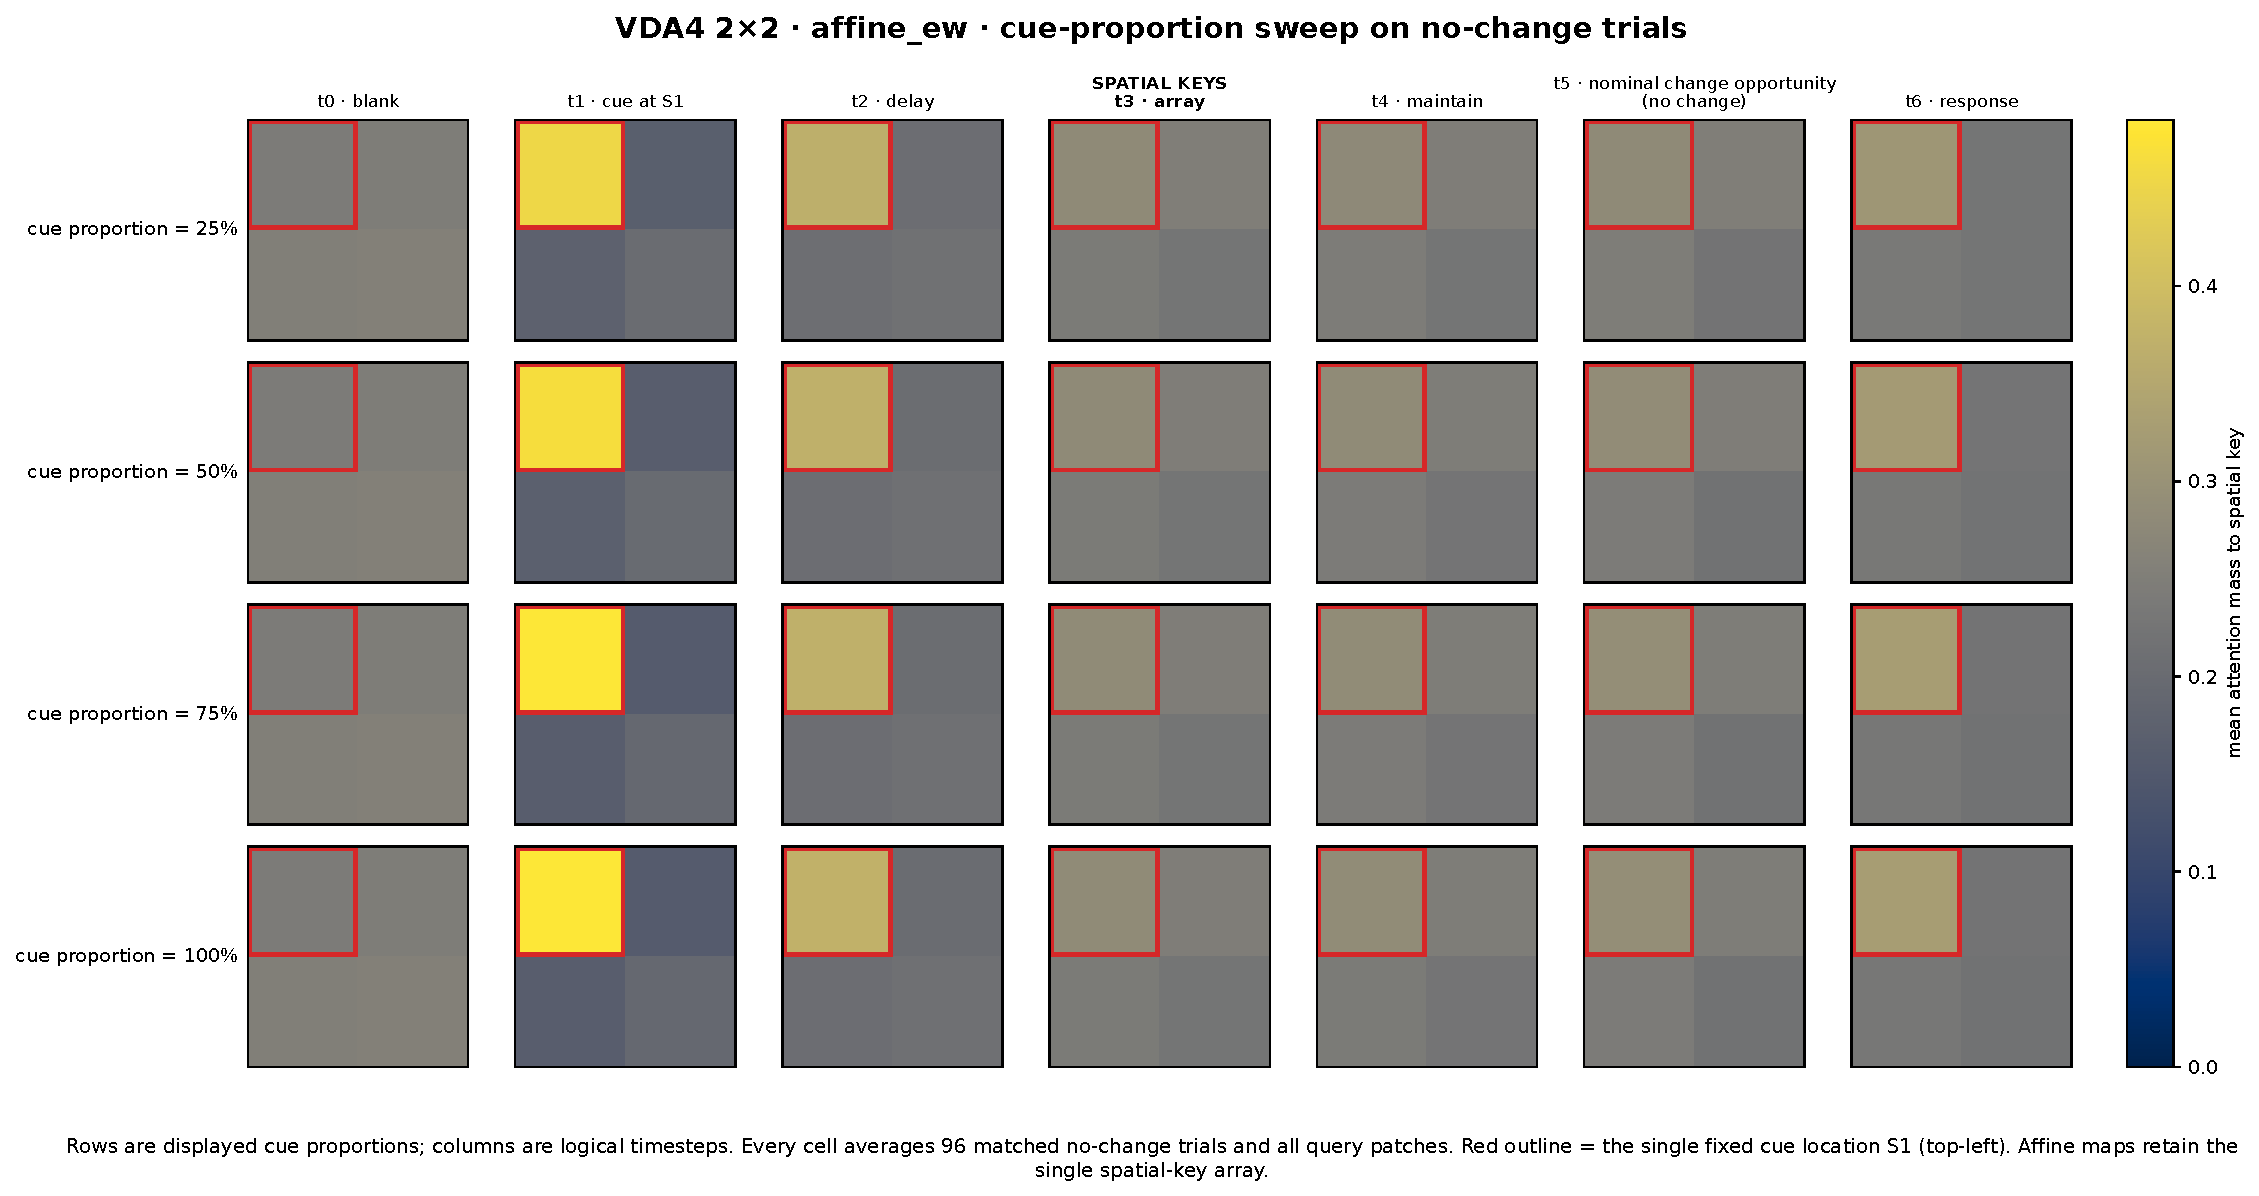
\includegraphics[width=0.96\linewidth]{first_wave_attention_vda4_affine_ew.pdf}
\captionof{figure}{\textbf{VDA4 affine attention on no-change trials.} \eclass{Checkpoint-recomputed descriptive measurement; 96 matched trials per displayed cue proportion.} Rows are cue proportions and columns are logical timesteps. At t5, the nominal change opportunity contains no physical change. Query patches are averaged, and the red outline identifies the fixed S1 cue location. Uniform mass over four spatial keys would assign 0.250 to each location. Colors share a zero-to-observed-maximum scale within this figure.}\label{fig:first-wave-attn-vda4-affine}
\end{center}\end{landscape}

\begin{landscape}\thispagestyle{plain}\begin{center}
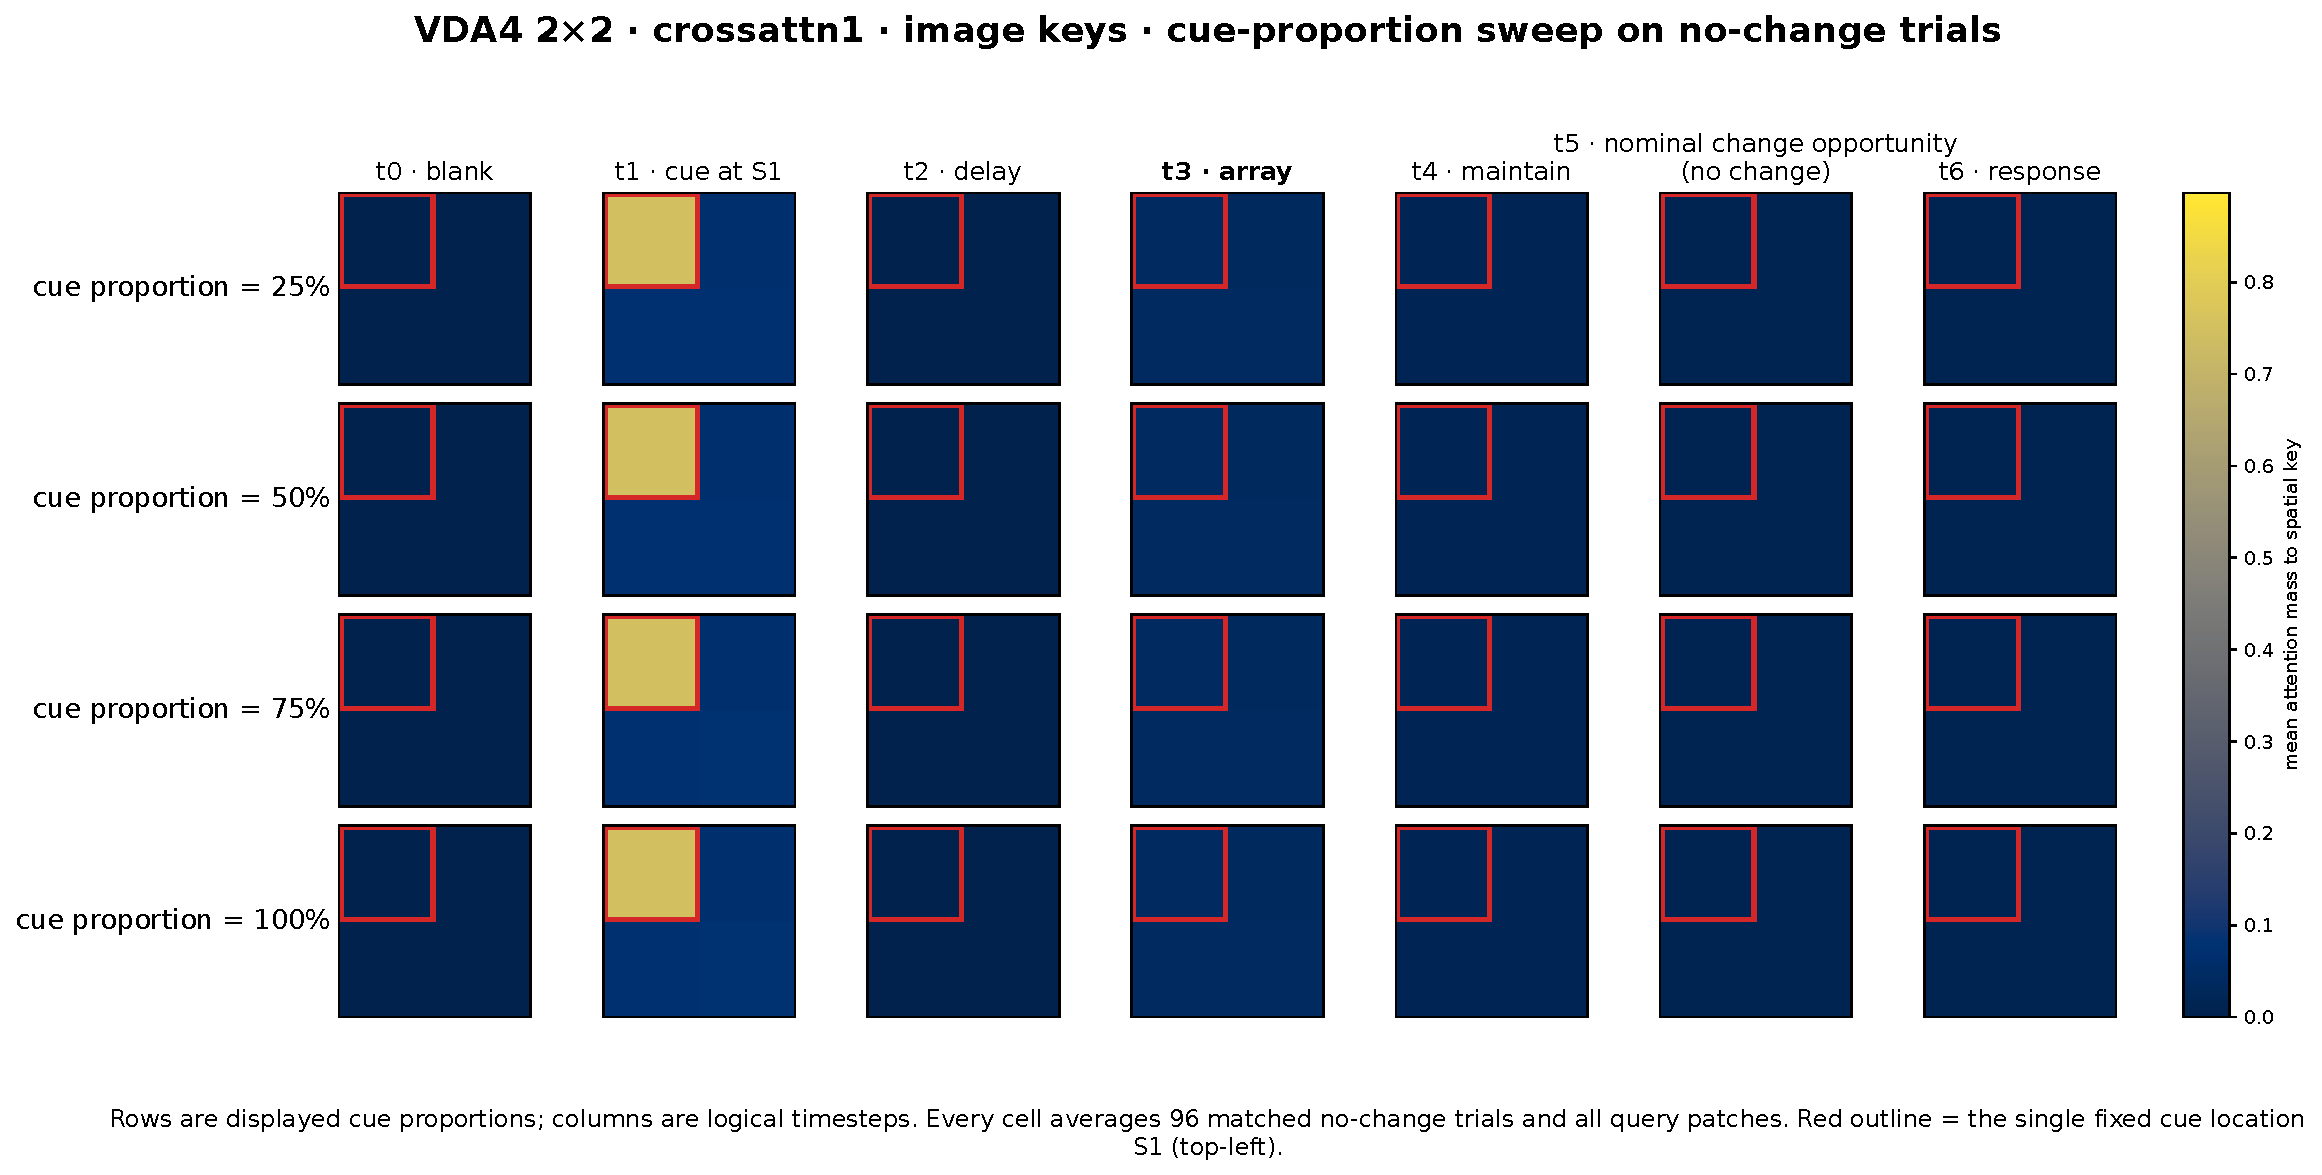
\includegraphics[width=0.96\linewidth]{first_wave_attention_vda4_crossattn1_image_keys.pdf}
\captionof{figure}{\textbf{VDA4 cross-attention to image keys on no-change trials.} \eclass{Checkpoint-recomputed descriptive measurement; 96 matched trials per displayed cue proportion.} This is the image-key $4\times7$ array: rows are cue proportions and columns are logical timesteps. At t5, the nominal change opportunity contains no physical change. Query patches are averaged and S1 remains the sole fixed cue location. Under uniform mass over all eight cross-attention keys, each spatial key receives $1/8=0.125$. This panel and its recurrent-memory companion share one zero-to-observed-maximum scale.}\label{fig:first-wave-attn-vda4-cross-image}
\end{center}\end{landscape}

\begin{landscape}\thispagestyle{plain}\begin{center}
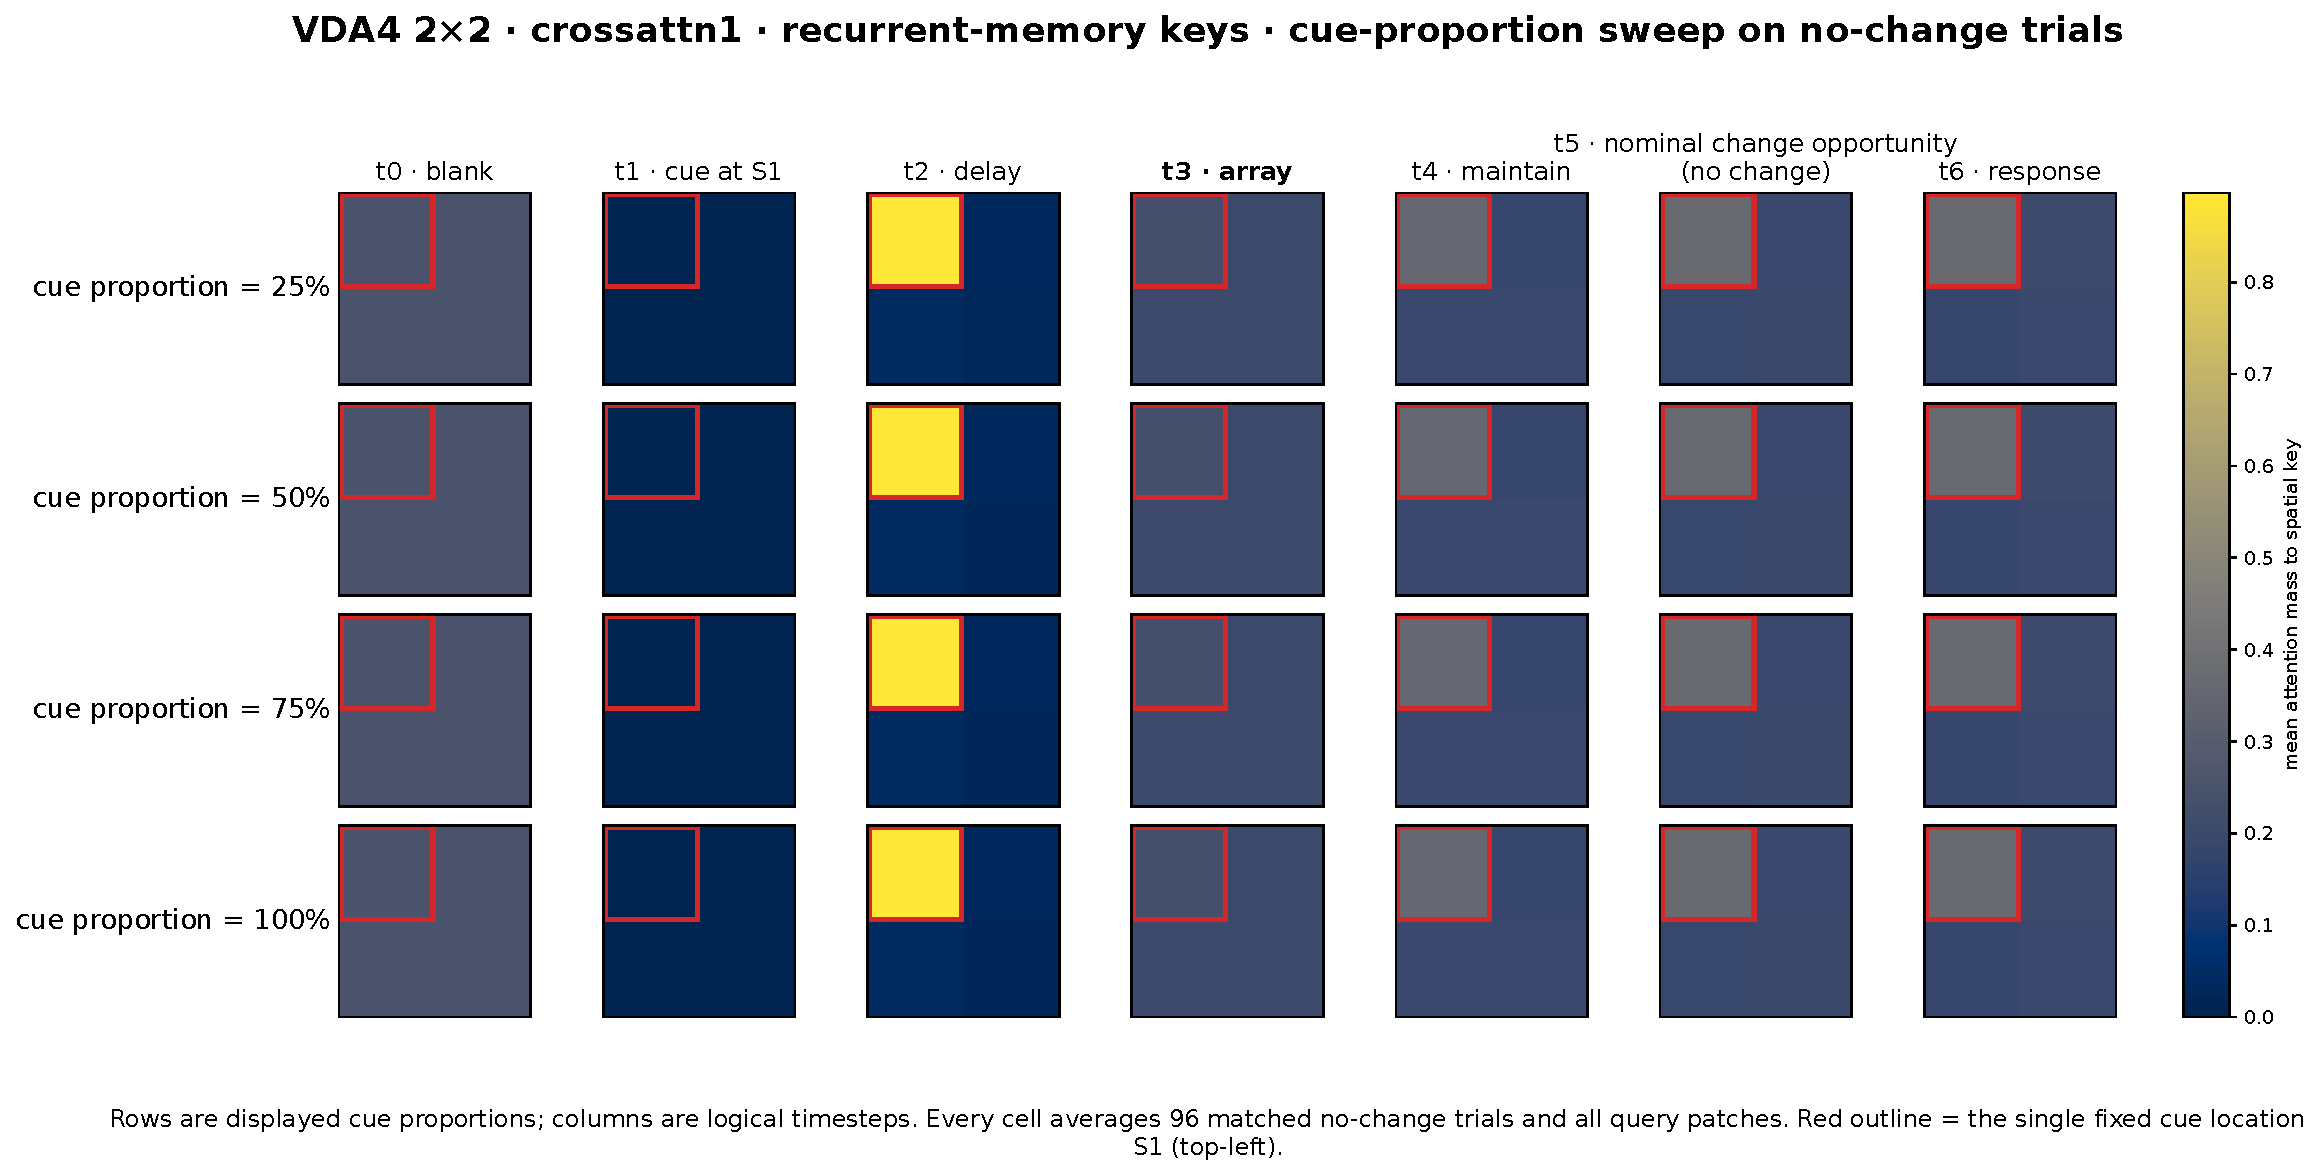
\includegraphics[width=0.96\linewidth]{first_wave_attention_vda4_crossattn1_recurrent_memory_keys.pdf}
\captionof{figure}{\textbf{VDA4 cross-attention to recurrent-memory keys on no-change trials.} \eclass{Checkpoint-recomputed descriptive measurement; 96 matched trials per displayed cue proportion.} This is the recurrent-memory-key $4\times7$ array: rows are cue proportions and columns are logical timesteps. At t5, the nominal change opportunity contains no physical change. Query patches are averaged and S1 remains the sole fixed cue location. Under uniform mass over all eight cross-attention keys, each spatial key receives $1/8=0.125$. This panel and its image-key companion share one zero-to-observed-maximum scale.}\label{fig:first-wave-attn-vda4-cross}
\end{center}\end{landscape}

\begin{landscape}\thispagestyle{plain}\begin{center}
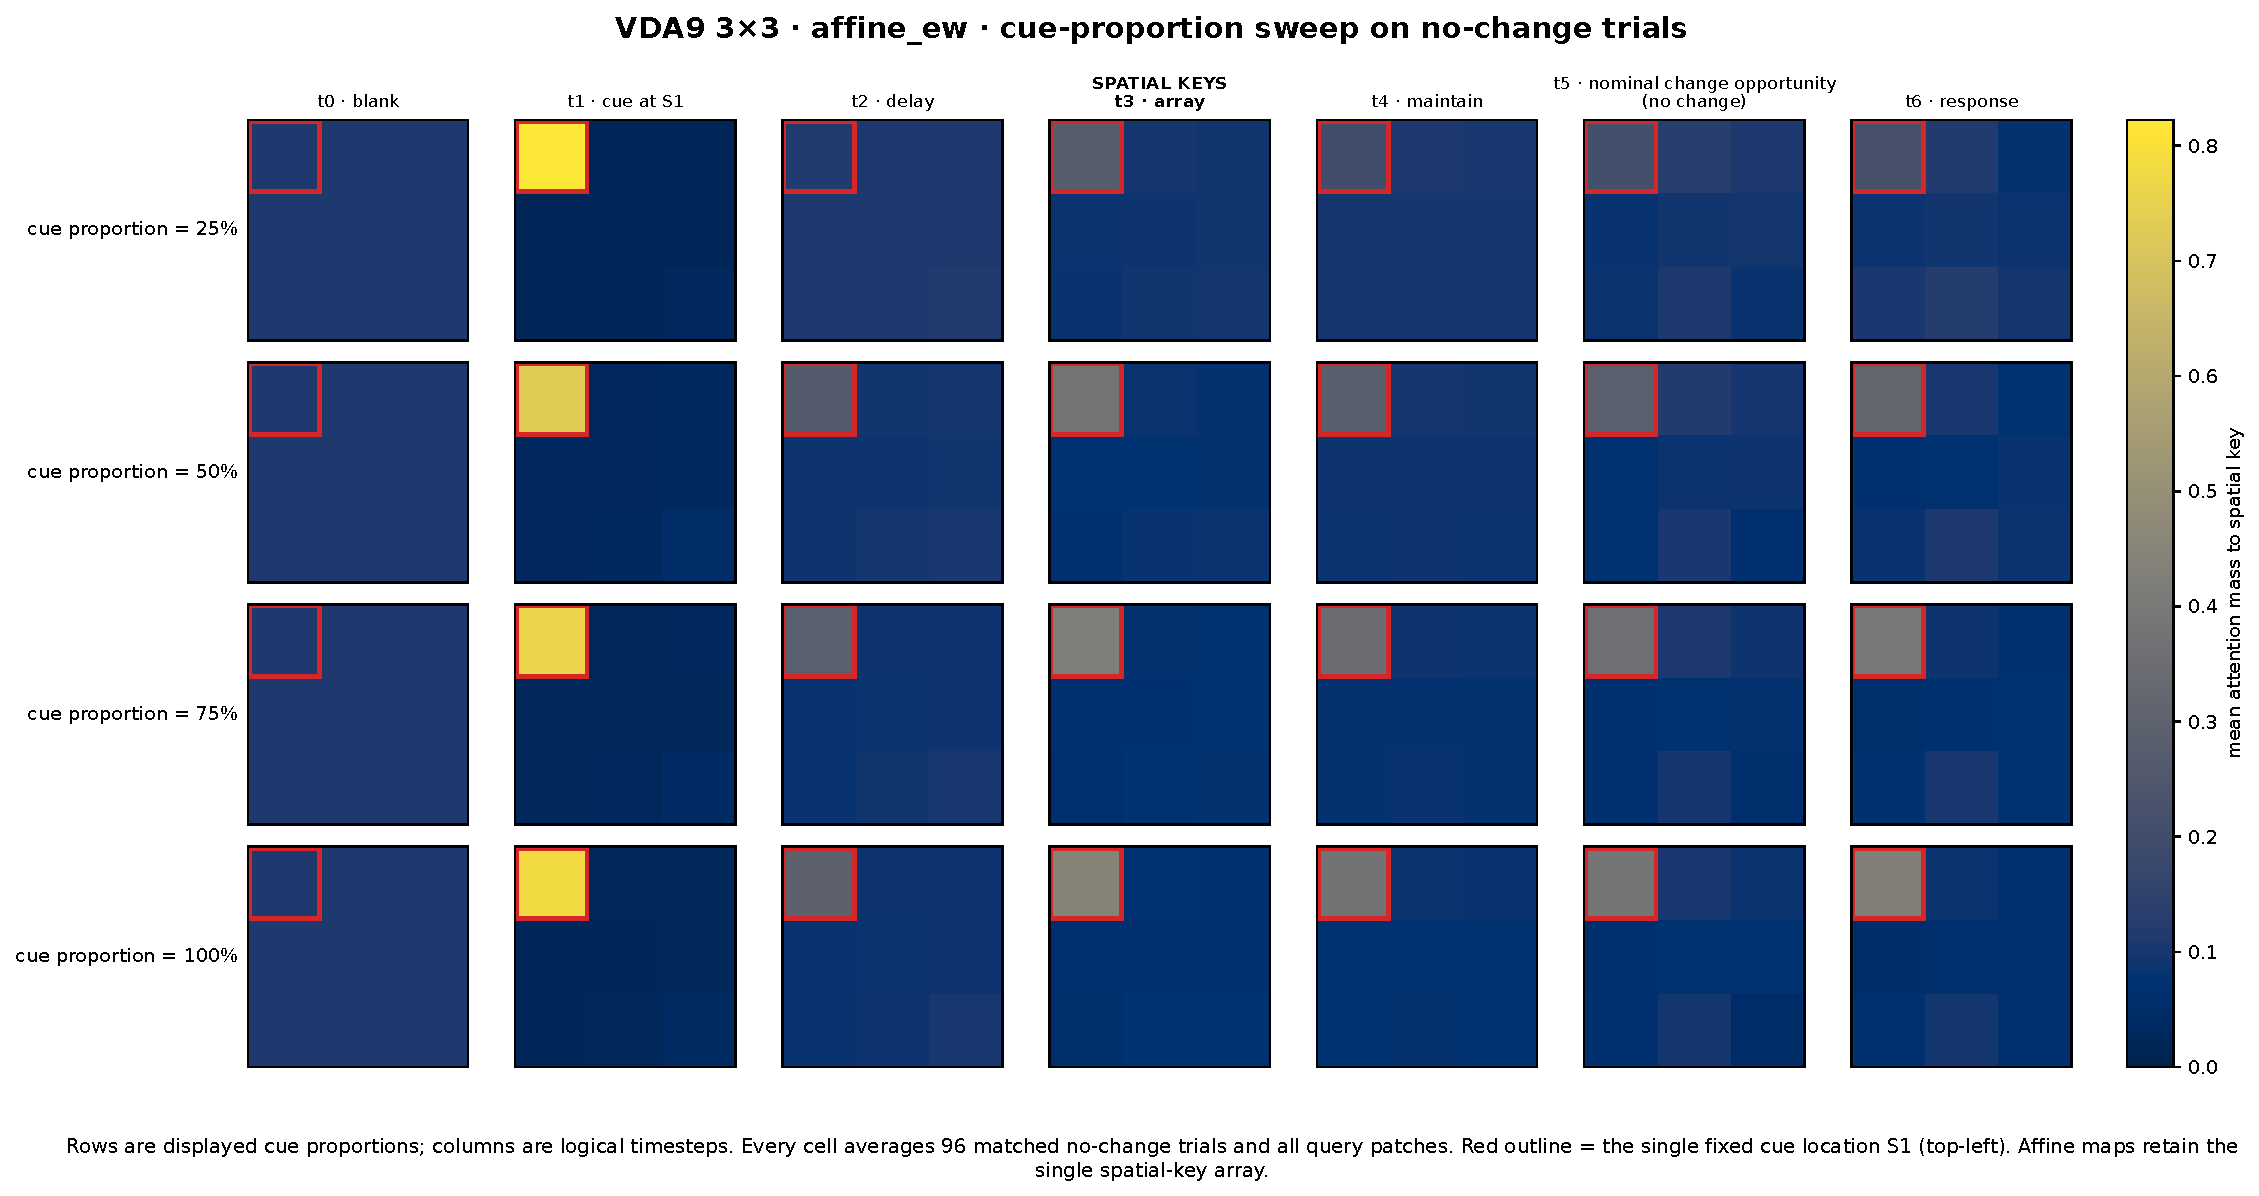
\includegraphics[width=0.96\linewidth]{first_wave_attention_vda9_affine_ew.pdf}
\captionof{figure}{\textbf{VDA9 affine attention on no-change trials.} \eclass{Checkpoint-recomputed descriptive measurement; 96 matched trials per displayed cue proportion.} Rows are cue proportions and columns are timesteps. At t5, the nominal change opportunity contains no physical change. Query patches are averaged, and the red outline identifies the fixed S1 cue location. Uniform mass over nine spatial keys would assign $1/9=0.111\ldots$ to each location. Colors share a zero-to-observed-maximum scale within this figure.}\label{fig:first-wave-attn-vda9-affine}
\end{center}\end{landscape}

\begin{landscape}\thispagestyle{plain}\begin{center}
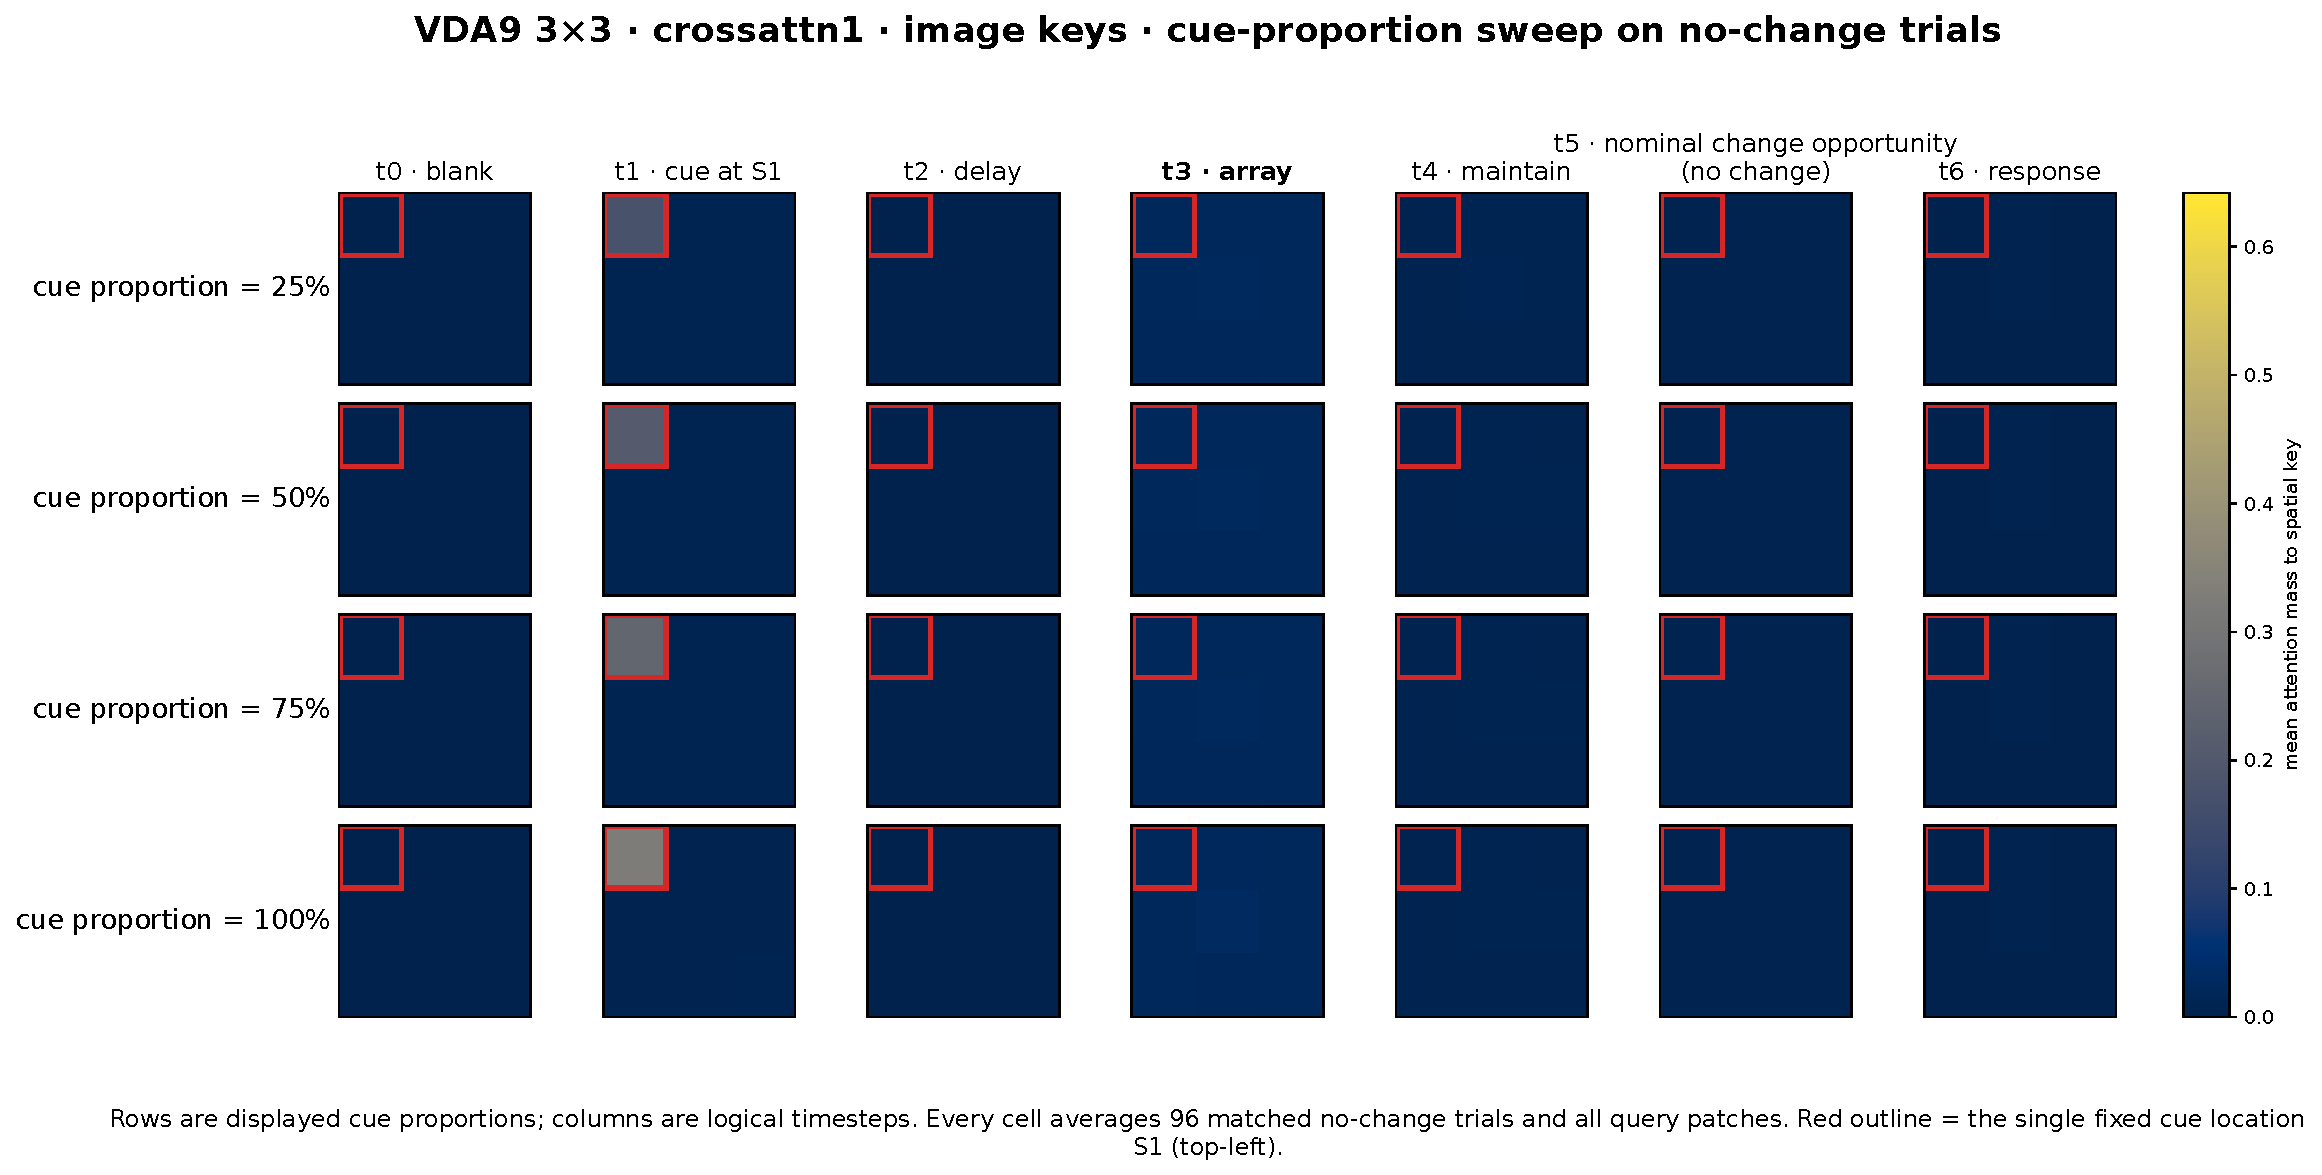
\includegraphics[width=0.96\linewidth]{first_wave_attention_vda9_crossattn1_image_keys.pdf}
\captionof{figure}{\textbf{VDA9 cross-attention to image keys on no-change trials.} \eclass{Checkpoint-recomputed descriptive measurement; 96 matched trials per displayed cue proportion.} This is the image-key $4\times7$ array: rows are cue proportions and columns are logical timesteps. At t5, the nominal change opportunity contains no physical change. Query patches are averaged and S1 remains the sole fixed cue location. Under uniform mass over all 18 cross-attention keys, each spatial key receives $1/18=0.0556\ldots$. This panel and its recurrent-memory companion share one zero-to-observed-maximum scale.}\label{fig:first-wave-attn-vda9-cross-image}
\end{center}\end{landscape}

\begin{landscape}\thispagestyle{plain}\begin{center}
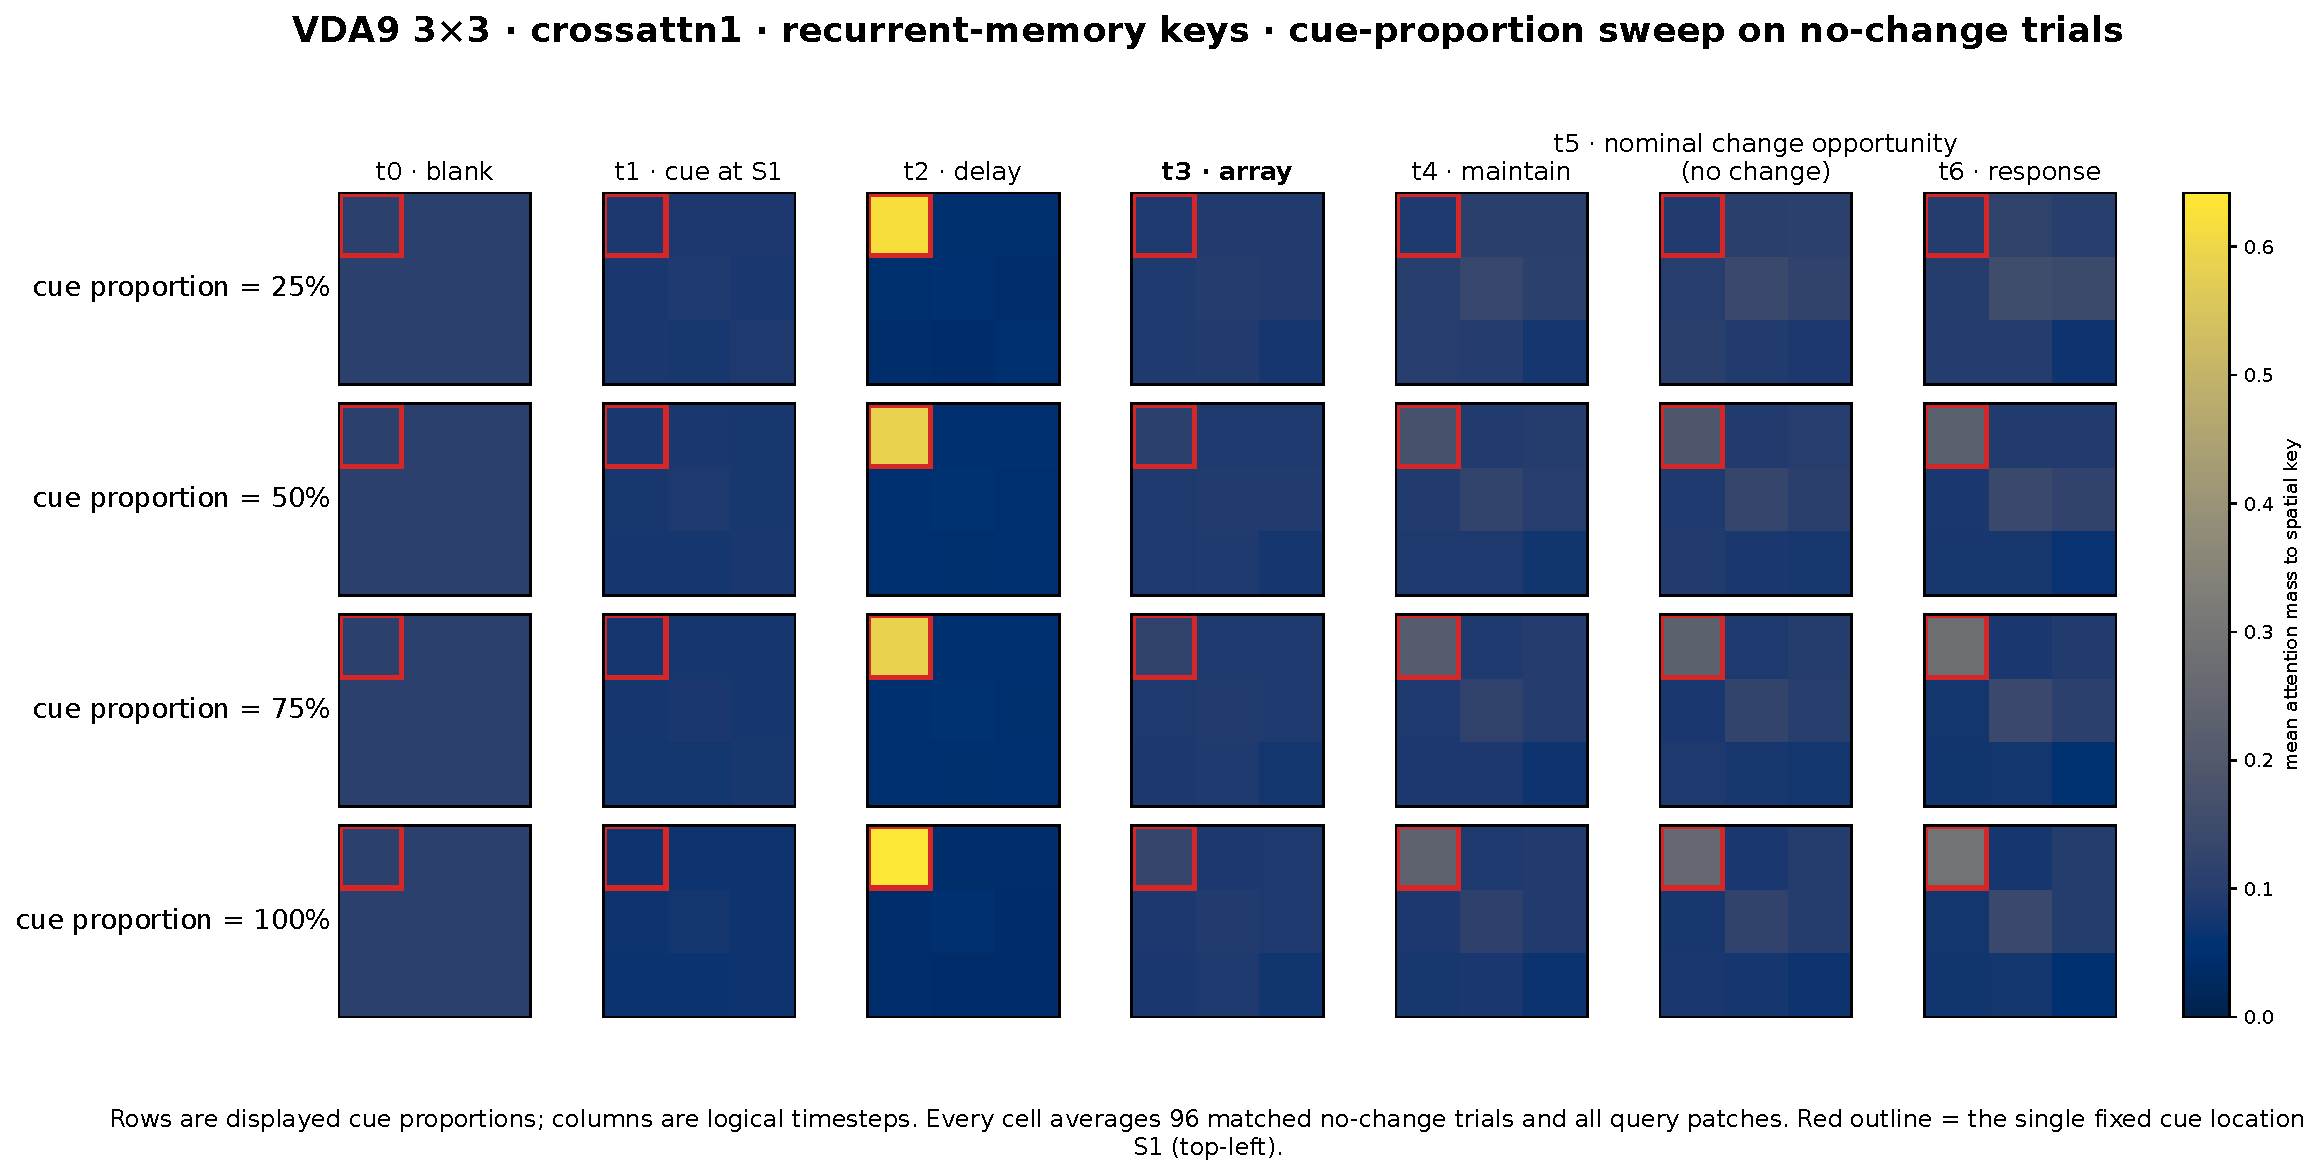
\includegraphics[width=0.96\linewidth]{first_wave_attention_vda9_crossattn1_recurrent_memory_keys.pdf}
\captionof{figure}{\textbf{VDA9 cross-attention to recurrent-memory keys on no-change trials.} \eclass{Checkpoint-recomputed descriptive measurement; 96 matched trials per displayed cue proportion.} This is the recurrent-memory-key $4\times7$ array: rows are cue proportions and columns are logical timesteps. At t5, the nominal change opportunity contains no physical change. Query patches are averaged and S1 remains the sole fixed cue location. Under uniform mass over all 18 cross-attention keys, each spatial key receives $1/18=0.0556\ldots$. This panel and its image-key companion share one zero-to-observed-maximum scale.}\label{fig:first-wave-attn-vda9-cross}
\end{center}\end{landscape}

\clearpage
\subsection{Three-panel psychometrics with finite-trial intervals}
Each psychometric point uses 300 evaluation trials. The ordinate is the probability of a qualifying change response: the first change declaration at logical frame 5 or later, divided by all evaluation trials. Panels A and B are fixed-location evaluations rather than draws from the historical location policy: the generator receives S1 or the bottom-right location as the explicit change index at every point while the displayed cue proportion is swept over 25\%, 50\%, 75\%, and 100\%. Panel C re-plots the 100\%-displayed endpoints from Panels A and B; it is a within-checkpoint fixed-location contrast, not an independent trial set or a naturally sampled 100\%-validity condition. Wilson 95\% intervals describe finite evaluation-trial uncertainty for one checkpoint; they do not estimate training-seed variation.

Across the four checkpoint families, change-response probability generally rises with orientation change. Fixed-S1 point estimates generally exceed fixed-bottom-right point estimates at intermediate magnitudes. The VDA9 cross-attention bottom-right curve remains below one at $30^\circ$ in Panel B and in its 100\%-displayed re-plot in Panel C. Those traces are identical by construction rather than independent replications; the value is retained as checkpoint behavior rather than ``corrected'' into saturation. These are finite-trial results from one checkpoint per family. Cross-family differences remain descriptive because weights, training histories, task geometry, and token count are not jointly controlled.

\begin{landscape}\thispagestyle{plain}\begin{center}
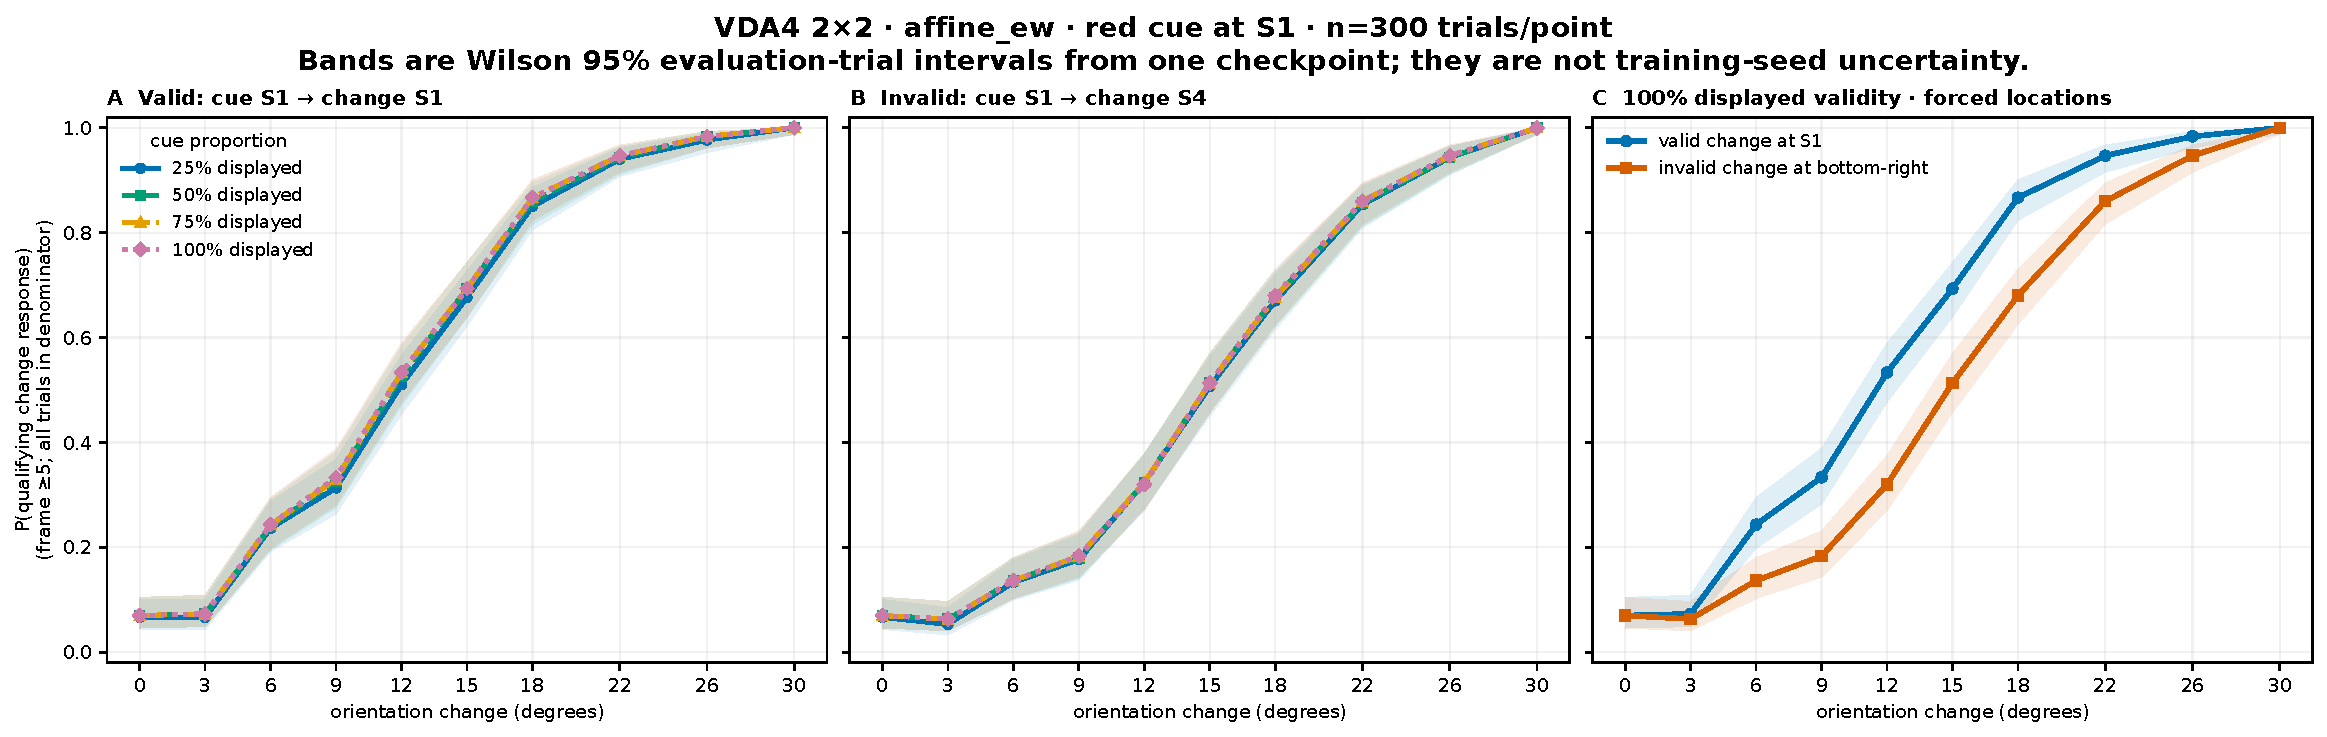
\includegraphics[width=0.84\linewidth]{first_wave_psychometric_vda4_affine_ew.pdf}
\captionof{figure}{\textbf{VDA4 affine psychometrics.} \eclass{Checkpoint-recomputed evaluation; 300 trials per point.} Panels A and B fix the change at S1 and S4, respectively, while sweeping displayed cue proportion. Panel C re-plots their 100\%-displayed endpoints; it is not an independent trial set. Bands are Wilson evaluation-trial intervals for one checkpoint.}\label{fig:first-wave-psych-vda4-affine}
\vspace{0.7em}
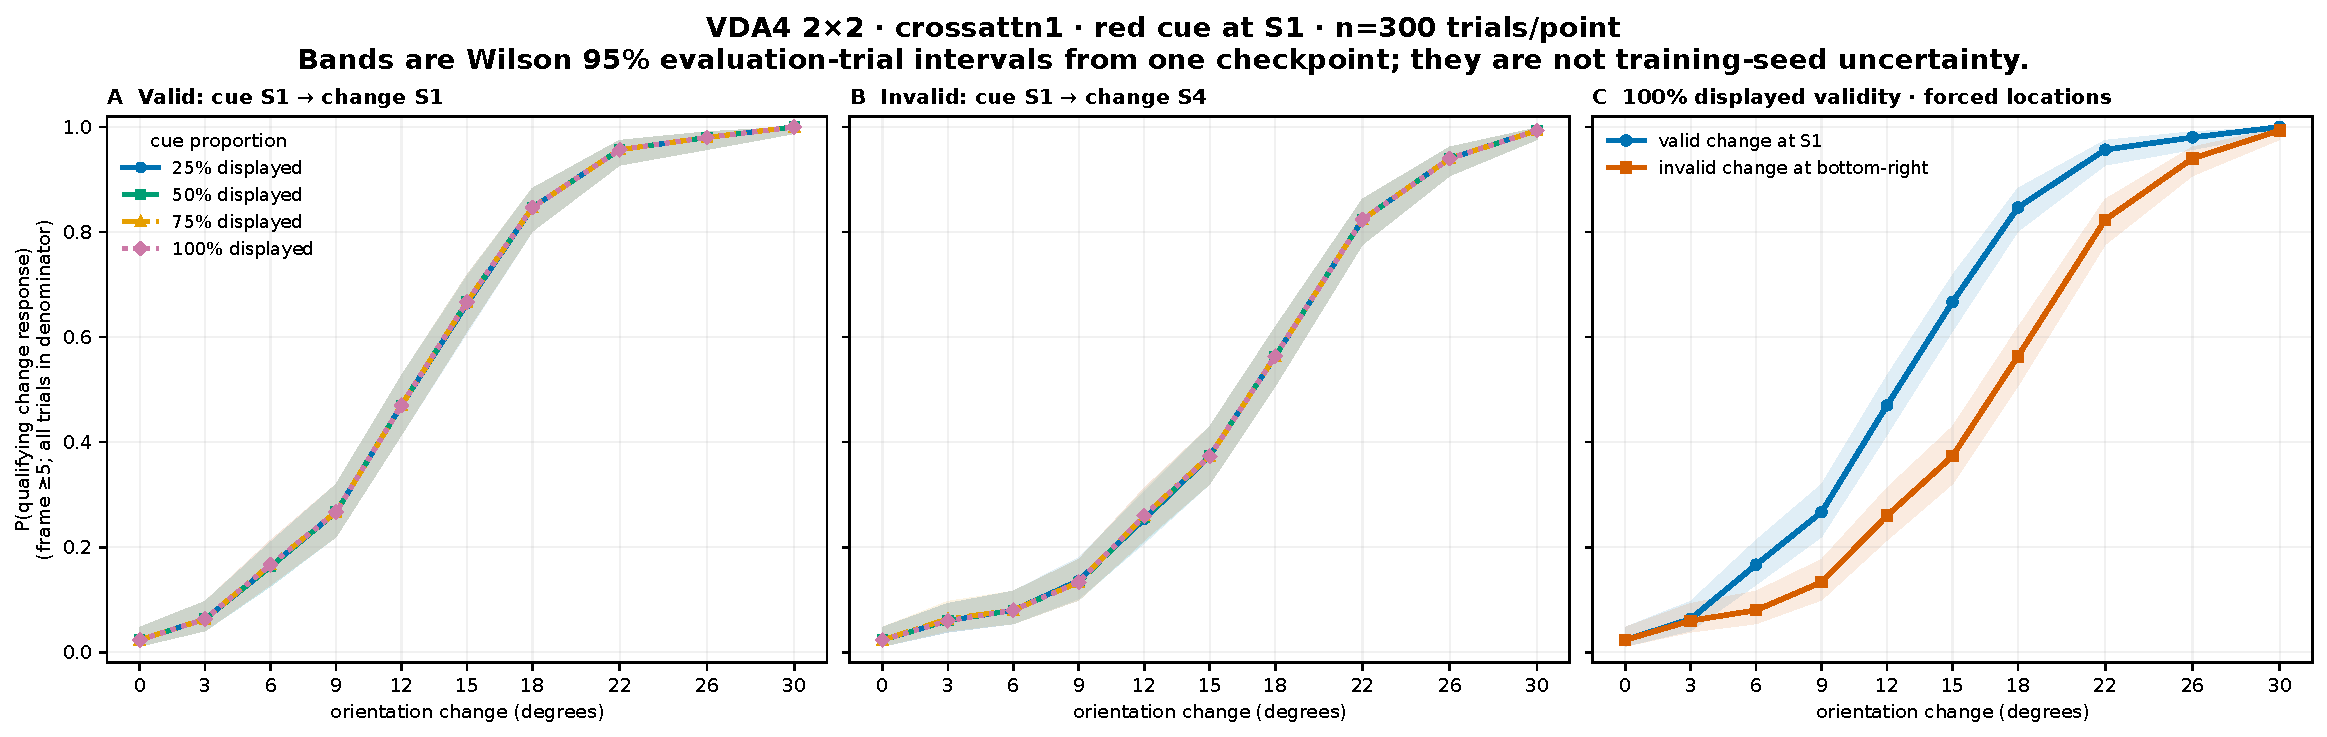
\includegraphics[width=0.84\linewidth]{first_wave_psychometric_vda4_crossattn1.pdf}
\captionof{figure}{\textbf{VDA4 cross-attention psychometrics.} \eclass{Checkpoint-recomputed evaluation; 300 trials per point.} The all-trial denominator, fixed S1 and S4 locations, and 100\%-displayed endpoint re-plot match Figure~\ref{fig:first-wave-psych-vda4-affine}. Separate checkpoints preclude a causal affine--cross-attention contrast.}\label{fig:first-wave-psych-vda4-cross}
\end{center}\end{landscape}

\begin{landscape}\thispagestyle{plain}\begin{center}
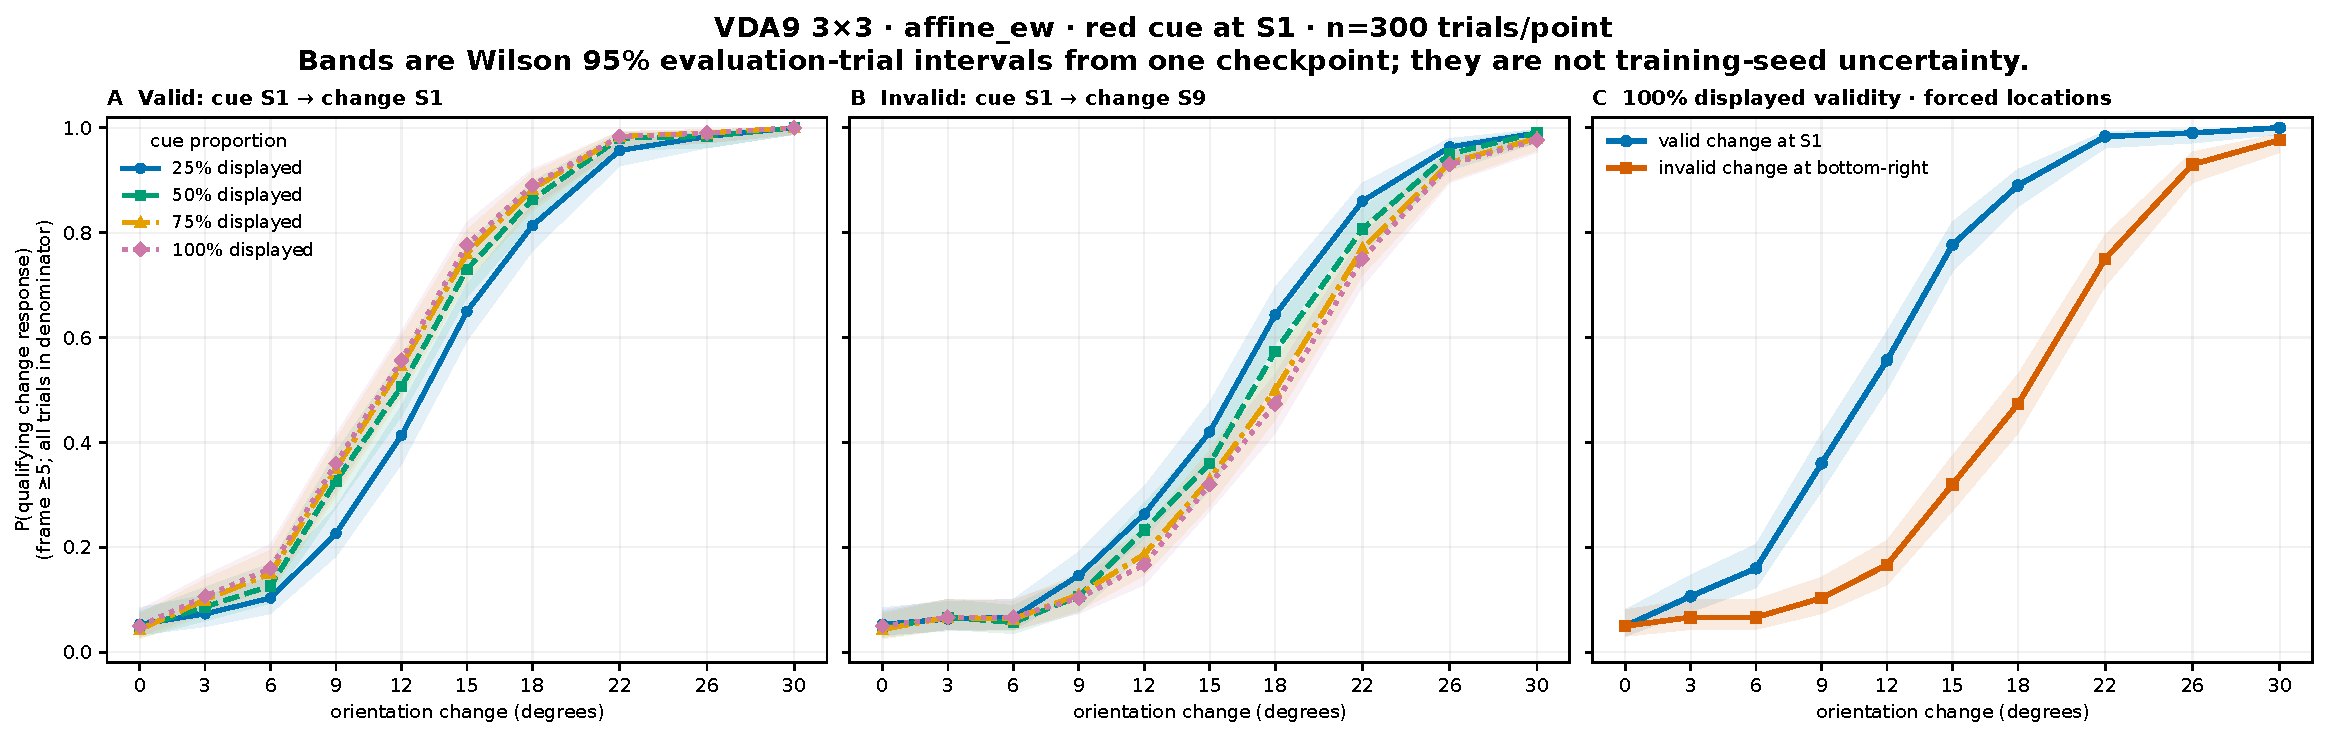
\includegraphics[width=0.80\linewidth]{first_wave_psychometric_vda9_affine_ew.pdf}
\captionof{figure}{\textbf{VDA9 affine psychometrics.} \eclass{Checkpoint-recomputed evaluation; 300 trials per point.} Panels A and B fix the change at S1 and S9, respectively; Panel C re-plots their 100\%-displayed endpoints. S9 is a specified bottom-right location, not a geometry-free ``opposing'' label. Wilson bands quantify finite evaluation-trial uncertainty only.}\label{fig:first-wave-psych-vda9-affine}
\vspace{0.7em}
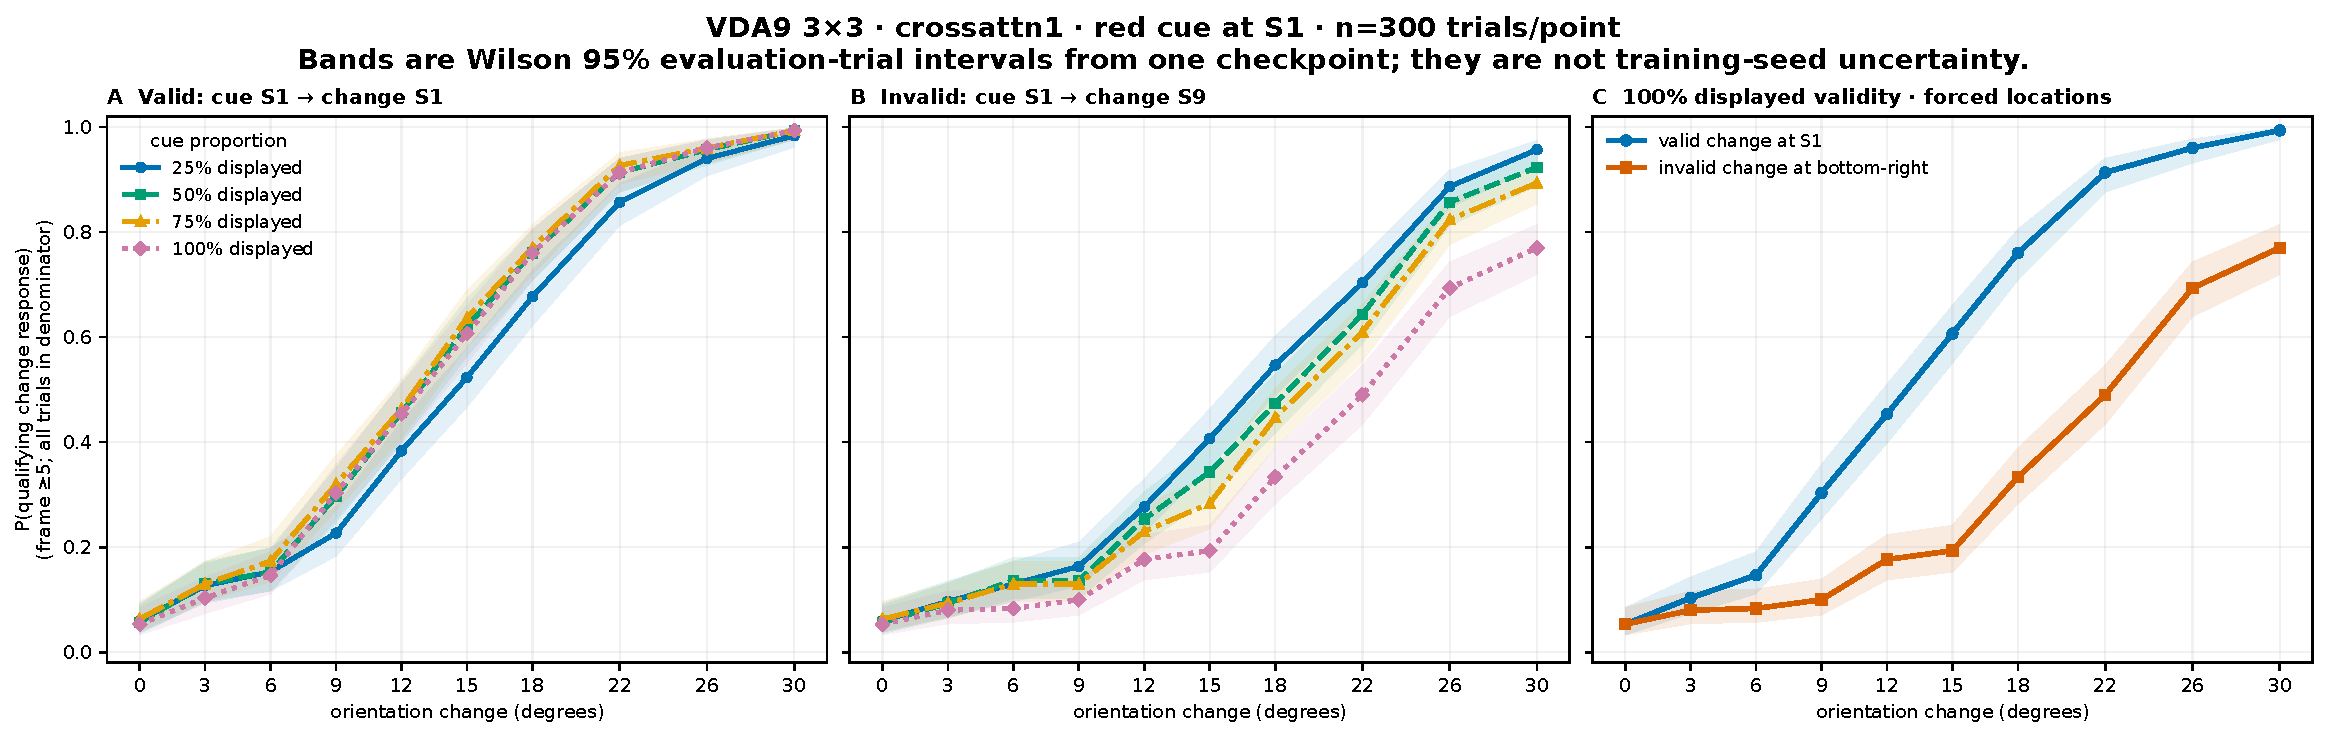
\includegraphics[width=0.80\linewidth]{first_wave_psychometric_vda9_crossattn1.pdf}
\captionof{figure}{\textbf{VDA9 cross-attention psychometrics.} \eclass{Checkpoint-recomputed evaluation; 300 trials per point.} The lower fixed-S9 response at large changes appears in Panel B and its 100\%-displayed endpoint re-plot in Panel C; the duplicate trace is by construction, not replication. It is a verified single-checkpoint result, not a replicated routing effect or evidence of a nine-item capacity boundary.}\label{fig:first-wave-psych-vda9-cross}
\end{center}\end{landscape}

\section{Matched-width behavioral, representational, and intervention battery}
\subsection{Why this battery follows the first wave}
The first wave establishes checkpoint-bound behavior and descriptive routing weights for four d128 checkpoints. It does not ask whether task variables can be read from the recurrent state or whether changing a routing input changes a decision endpoint. The matched battery therefore asks three successive questions: do behavioral point estimates differ between configured checkpoints, what information can a held-out probe read, and does an assigned routing-logit intervention alter model sensitivity? It reuses the exact d128 VDA4 and VDA9 checkpoints from the first wave, adds two VDA1 d128 checkpoints, and pairs each with a separately trained d256 checkpoint. Width is the descriptive grouping contrast, not the causal manipulation.

Here width is the configured recurrent memory dimension \texttt{d\_mem}. Each patch location carries xLSTM states $H$, $C$, $N$, and $M$ with 128 or 256 coordinates. The actor and critic read the locations after flattening, so their input dimension is the number of tokens times \texttt{d\_mem}. Sensory token width, task geometry, routing family, and iteration are fixed within each admitted pair; learned weights and training trajectories are not.

\begingroup\small
\captionof{table}{\textbf{Configured d128/d256 checkpoint comparison.} Task geometry, routing family, sensory token width, and iteration are held fixed within each admitted pair; recurrent width, flattened readout dimension, parameter count, learned weights, and training trajectory are not all matched.}\label{tab:width-comparison}
\begin{tabularx}{\textwidth}{@{}p{4.0cm}Y Y Y@{}}
\toprule
Quantity & d128 checkpoint & d256 checkpoint & Pairwise status\\
\midrule
Per-location recurrent state & $H,C,N,M$: 128 coordinates & $H,C,N,M$: 256 coordinates & Configured difference\\
Flattened actor/critic input & 512 (four tokens) or 1152 (nine) & 1024 (four tokens) or 2304 (nine) & Consequence of \texttt{d\_mem}\\
Sensory token width & 140 (four-token tasks) or 145 (VDA9) & Same as d128 & Held fixed within pair\\
Trainable parameters & 2.200--2.545 million & 2.805--3.509 million & Task- and routing-dependent\\
Task geometry and tokens & VDA1/VDA4: four; VDA9: nine & Same as d128 & Held fixed within admitted pair\\
Checkpoint & Iteration 19999 & Iteration 19999 & Separately trained weights\\
\bottomrule
\end{tabularx}
\endgroup

Twelve immutable result files, one per task--routing--width cell, bind checkpoint bytes, executable source, runtime, protocol arrays, and deterministic trial fields. Both VDA2 routing-specific width pairs are blocked because the available d256 checkpoints have two tokens whereas the canonical d128 checkpoints have four. VDA9 cross-attention d256 fails the registered behavioral acceptance threshold, so that pair contributes no width contrast. The resulting five pairs are checkpoint comparisons, not independent-seed populations.

\subsection{Observed behavior}
At $14^\circ$, the clearest opposing contrast is a 21-percentage-point increase for VDA1 cross-attention versus a 13-percentage-point decrease for VDA4 cross-attention when d256 is compared with d128. The other three admitted pairs likewise do not produce a common direction. Each psychometric point contains 300 forced valid-location change trials at displayed validity 0.75; Table~\ref{tab:absolute-behavior} reports every absolute constituent curve behind Figure~\ref{fig:matched-width}A. No interval is shown for these cross-checkpoint differences, and the design cannot separate architecture, training-run variation, and finite evaluation noise.

\subsection{Held-out readout from the recurrent state}
Each result file contains 900 trials, balanced as 450 change-present and 450 no-change trials, and uses four fixed folds. All three reported decoder scores are four-fold balanced accuracies. Change-occurrence decoding is binary over all 900 trials, with chance 0.5. Realized change location uses only the 450 change-present trials: VDA4 is four-class, with class counts 225, 75, 75, and 75 and balanced-accuracy chance 0.25; VDA9 is nine-class, with 225 cued-location samples and 28--29 samples at each of eight uncued locations and balanced-accuracy chance $1/9\simeq0.111$. Cued-versus-uncued change location is binary over those same 450 trials, with 225 samples per class and balanced-accuracy chance 0.5. Both location targets are undefined for singleton VDA1. Within each fold and timestep, scaling and PCA are fitted only on the training partition before a regularized logistic probe is fitted in a common 128-dimensional space. Timestep t0 is omitted because the pre-stimulus states have zero variance and score at chance. Warning localization came from a reviewed process log that was not retained in the upstream hash-bound evidence tree. Native cued-change trajectories for VDA9 affine d256 and VDA9 cross-attention d128 are therefore omitted conservatively; finite matched PCA-128 outputs are reported without claiming a hash-bound no-warning ledger.

The absolute t6 scores are needed to interpret the differences in Figure~\ref{fig:matched-width}. Change occurrence is strongly readable in every admitted checkpoint, with balanced accuracy from 0.761 to 0.902. Location-conditioned readout is more variable: VDA9 affine d256 realized-location balanced accuracy is 0.499, substantially above the nine-class balanced-accuracy reference $1/9=0.111$ despite the 225/450 majority class, but below its d128 counterpart at 0.654; other defined scores reach 0.958. These foldwise values are descriptive scores from separately trained checkpoints, not independent training replicates, and no uncertainty interval is reported.

\begingroup\small
\captionof{table}{\textbf{Final-timestep held-out decoder scores.} Entries are four-fold balanced accuracies at t6 in d128/d256 order; location targets are undefined for singleton VDA1.}\label{tab:decoder-scores}
\begin{tabularx}{\textwidth}{@{}p{3.0cm}p{2.2cm}Y Y Y@{}}
\toprule
Task & Routing & Change occurrence balanced accuracy d128/d256 & Change location balanced accuracy d128/d256 & Cued vs uncued balanced accuracy d128/d256\\
\midrule
VDA1 & affine & .893 / .902 & undefined & undefined\\
VDA1 & cross-attention & .897 / .888 & undefined & undefined\\
VDA4 & affine & .830 / .879 & .616 / .900 & .845 / .958\\
VDA4 & cross-attention & .818 / .833 & .842 / .792 & .936 / .907\\
VDA9 & affine & .761 / .792 & .654 / .499 & .889 / .831\\
\bottomrule
\end{tabularx}
\endgroup

The corresponding d256-minus-d128 differences vary in sign. For example, VDA4 affine differs by 0.285 for change location, whereas VDA4 cross-attention differs by $-0.050$. Thus a wider checkpoint does not expose uniformly more linearly decodable information in these selected pairs. The scores establish information available to the stated readout at t6; they do not establish delay maintenance, policy use, or necessity.

\subsection{Within-checkpoint key-logit intervention}
From logical frames 5 through 6, the intervention adds $b\in\{-6,-3,0,3,6\}$ to selected routing scores for every query:
\begin{equation}
s'_{tqk}=s_{tqk}+b\,\mathbf{1}[t\geq5]\,\mathbf{1}[k\in\mathcal{K}_{\mathrm{cue}}].
\end{equation}
For affine routing, $\mathcal{K}_{\mathrm{cue}}$ contains the cued image key. For cross-attention it contains both the cued image key and the corresponding memory key. Bias values are comparable across widths within a routing family, but not as equal intervention doses across routing families because the target sets differ. The same numeric offset need not produce the same change in softmax allocation across checkpoints, and achieved attention mass is neither assigned nor standardized.

Each bias, condition, and checkpoint has 250 trials. A valid or invalid hit is a declaration at frame 5 or 6 on the corresponding change trial; a false alarm is any declaration on a no-change trial. Rates are clipped to $[1/(2n),1-1/(2n)]$ before
\begin{equation}
d'=\Phi^{-1}(H)-\Phi^{-1}(F), \qquad c=-\tfrac12\left[\Phi^{-1}(H)+\Phi^{-1}(F)\right].
\end{equation}
The battery retains both $d'$ and criterion $c$, but this manuscript evaluates only $d'$. For condition $x$, the plotted quantity is
\begin{equation}
D_{w,x}(b)=d'_{w,x}(b)-d'_{w,x}(0),\qquad
W_x(b)=D_{256,x}(b)-D_{128,x}(b).
\end{equation}
Thus the assigned logit offset estimates a within-checkpoint intervention effect on response counts and the derived signal-detection endpoint, while $W_x(b)$ compares those effects across separately trained checkpoints. It does not establish that biological or model-level ``attention allocation'' changed by a calibrated amount.

One representative sign reversal occurs at bias $-6$. For VDA4 affine, the within-checkpoint constituents are $D_{128,\mathrm{valid}}=-1.384$ and $D_{256,\mathrm{valid}}=-0.491$, giving $W_{\mathrm{valid}}=0.893$; for VDA4 cross-attention they are $-0.544$ and $-0.736$, giving $W_{\mathrm{valid}}=-0.192$. Table~\ref{tab:clamp-constituents} reports every $D_{w,x}(b)$ behind Figure~\ref{fig:matched-width}C--D. Invalid-change effects are undefined for singleton VDA1. Aggregate counts do not retain trial identities, so paired intervals are unavailable; no unpaired or model-based interval is presented. Across the behavioral, t6 readout, and key-logit intervention analyses, the wider checkpoint is not consistently better, does not consistently expose more linearly decodable information, and is not consistently more responsive to the intervention.

\begin{landscape}\thispagestyle{plain}\begin{center}
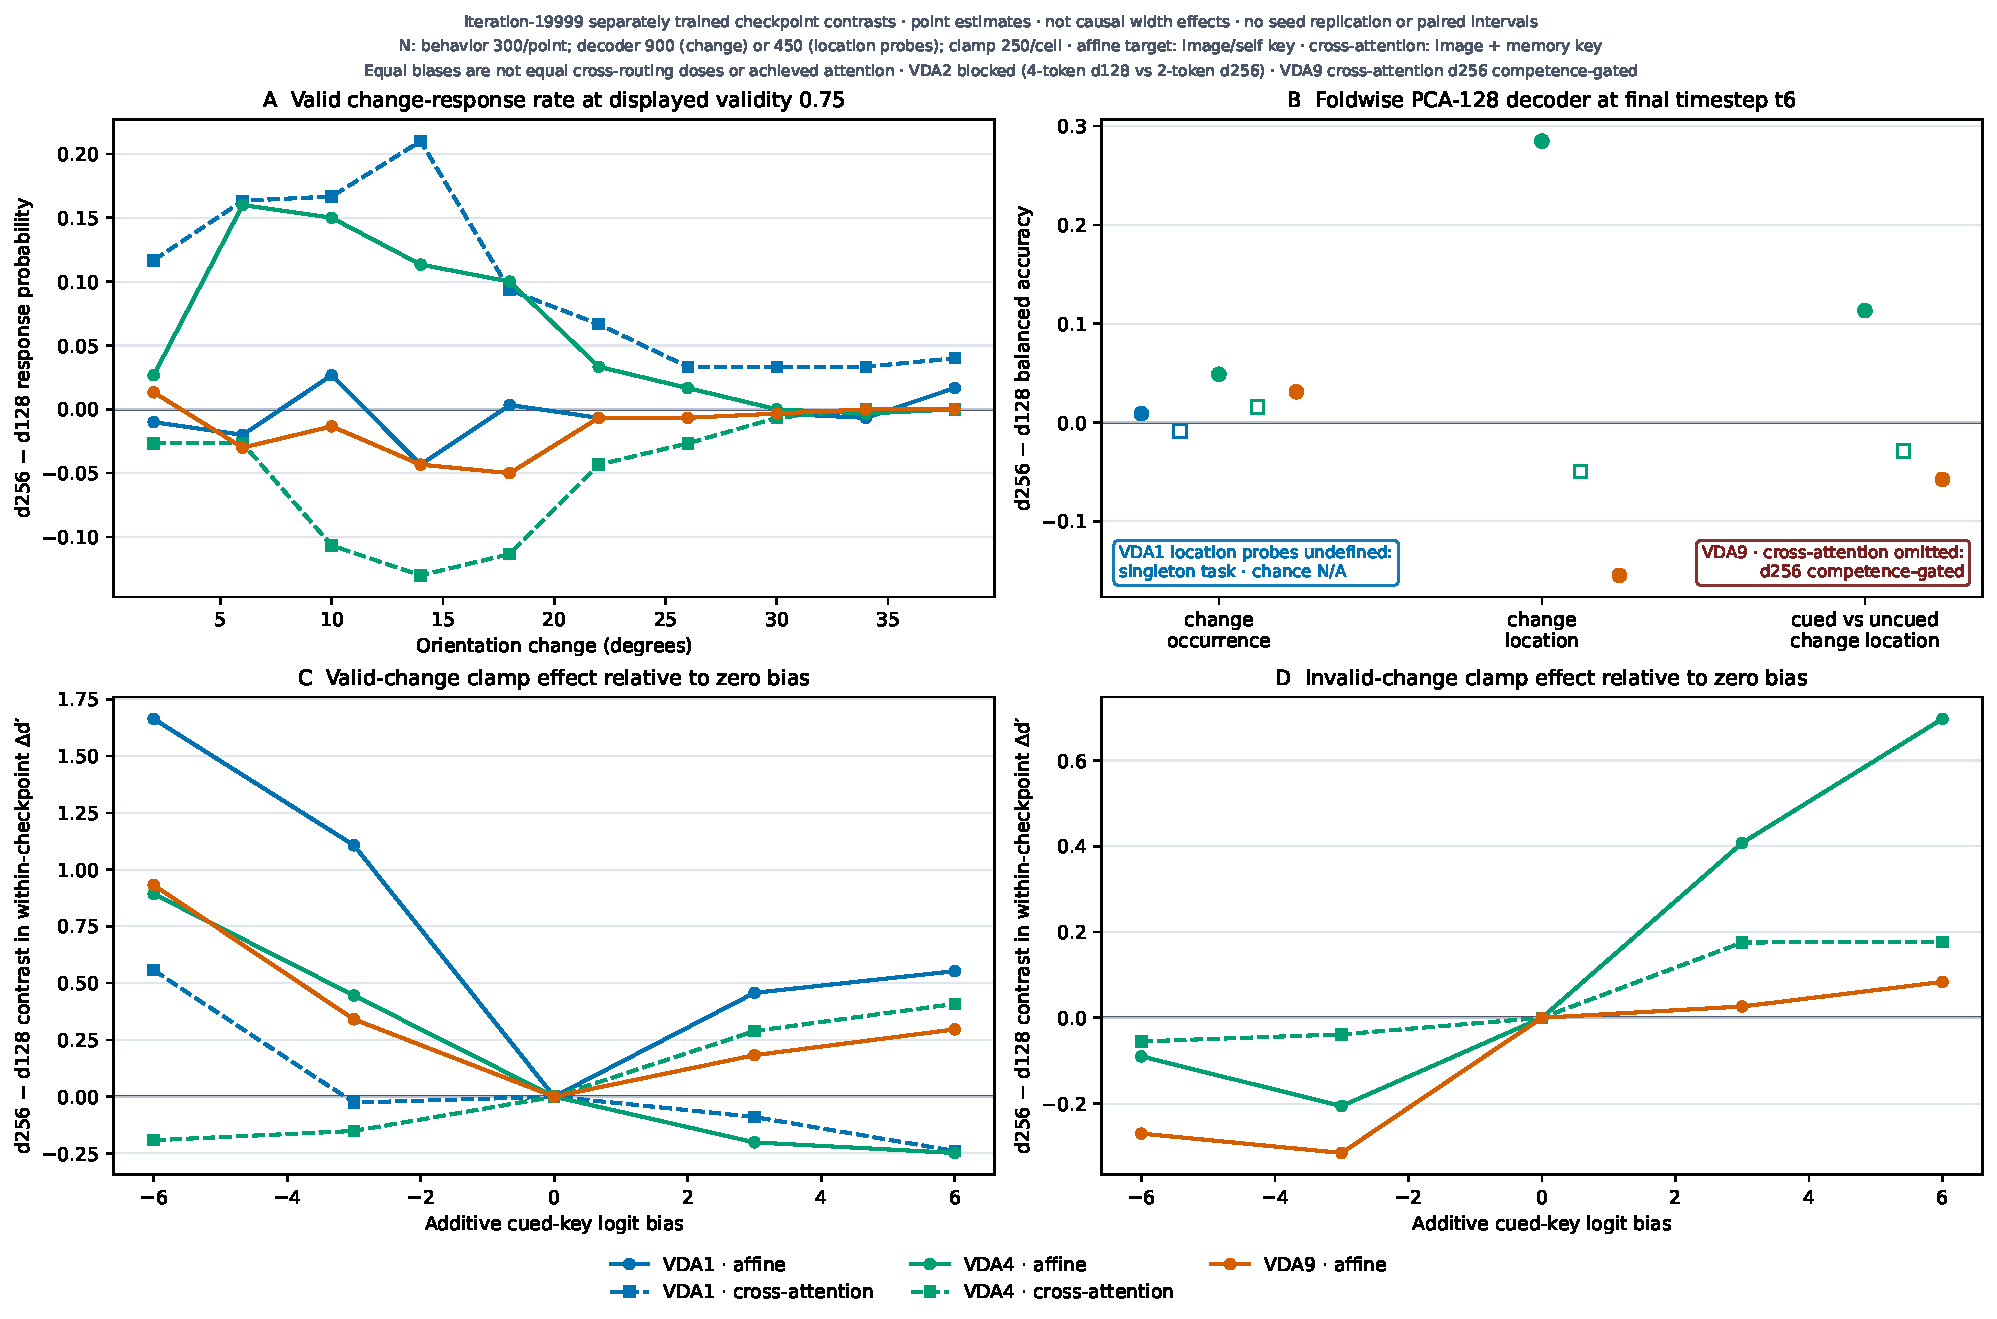
\includegraphics[width=0.68\linewidth]{matched_width_summary.pdf}
\captionof{figure}{\textbf{Matched-width checkpoint summary.} \eclass{Checkpoint-recomputed descriptive and model-intervention evidence.} All ordinates compare separately trained iteration-19999 d256 and d128 checkpoints; across panels, the five admitted pairs do not show a consistent wider-is-better direction. \textbf{Panel map.} A shows valid-location response differences at displayed validity 0.75 (300 trials per point), and Table~\ref{tab:absolute-behavior} gives the absolute curves. B shows t6 foldwise PCA-128 balanced-accuracy differences. C and D show cross-checkpoint differences in the within-checkpoint $d'$ change from zero bias (250 trials per cell), and Table~\ref{tab:clamp-constituents} gives every constituent. \textbf{Support and references.} Zero, not chance, is B's plotted reference because its ordinate is d256 minus d128. Unplotted absolute chance is 0.5 for binary change occurrence over 900 trials, 0.25 or $1/9$ for realized location over 450 change-present VDA4 or VDA9 trials, and 0.5 for cued-versus-uncued location over the same 450 trials. For scale, VDA9 affine d256 realized-location balanced accuracy is 0.499 versus $1/9=0.111$ chance (d128: 0.654). \textbf{Interpretive limits.} Structurally chance t0 points and native trajectories without a hash-bound warning ledger are omitted. Affine routing biases the cued image key; cross-attention biases that image key and its memory key, so equal biases are not calibrated cross-routing doses or achieved-attention allocations. VDA1 invalid effects are undefined; VDA2 is blocked by a token-geometry mismatch; and VDA9 cross-attention is competence-gated. Aggregate counts do not preserve trial identities, so paired intervals are unavailable.}\label{fig:matched-width}
\end{center}\end{landscape}

\boundary{The completed battery supports checkpoint-specific behavioral point estimates, absolute t6 readout scores, and effects of an assigned key-logit offset within evaluated checkpoints. Across five admitted pairs, the d256-minus-d128 point estimates do not share one direction. The design cannot determine whether that variation reflects architecture, training-run variation, or finite evaluation noise. It does not estimate a causal width effect, human working-memory capacity, training-seed replication, or biological homology. The targeted summary does not promote the 952 source-panel coverage dispositions.}

\section{Neuroscience correspondence without anatomical inflation}
The model task belongs to a real experimental tradition, but correspondence must be local.

\paragraph{Sensitivity versus criterion.} Carrasco's synthesis distinguishes improved discriminability from faster or more liberal responding and separates contrast-gain, response-gain, spatial-resolution, and external-noise accounts \cite{carrasco2011}. Luo and Maunsell show why those alternatives cannot be collapsed into ``attention'': a more liberal declaration policy can raise hit rate without improving sensory evidence \cite{luo2018}. The historical aggregates and first wave lack a criterion/sensitivity decomposition. The matched battery retains model $d'$ and criterion at each key-logit dose, but only $d'$ is analyzed here. A criterion analysis and an external-noise manipulation are therefore required before the natural cue effect can be assigned to sensitivity, policy, or both; ``gain'' remains descriptive rather than a biological mechanism diagnosis.

\paragraph{Event-aligned representation versus neural dynamics.} Herman and Krauzlis reported cue- and detection-related superior-colliculus activity that covaried with manual reports and preceded response \cite{herman2017}. Panichello and Buschman reported shared prefrontal population geometry across controlled attention and working-memory selection tasks \cite{panichello2021}. At t6, the reported model decoders read change occurrence and realized change location; they do not decode cue location or establish a delay-period code. Event-aligned hit/miss trajectories, delay-spanning decoders, and response-latency analyses would test signal-to-response and domain-general correspondences without establishing anatomical homology. Likewise, Luck and Vogel motivate a set-size question at the level of integrated objects, not a theorem that a recurrent tensor has four slots \cite{luck1997}. A controlled fixed-grid multi-seed series with an operational capacity estimand is still required.

\paragraph{Model perturbation versus biological causal intervention.} The retinotopic logic of frontal-eye-field microstimulation motivates spatially matched perturbations \cite{moore2003}, but the routing clamp is an assigned model intervention, not electrical stimulation of a biological circuit. Its within-checkpoint $d'$ effect does not identify a causal width effect or a biological mechanism. Source-matched location controls, criterion analysis, achieved-allocation calibration, and biological measurements would be needed to discriminate a model-level correspondence from analogy.

\boundary{The admissible language is ``model-level counterpart,'' ``structurally analogous,'' or ``corresponds to.'' No result in this manuscript identifies a tensor as FEF, SC, LPFC, or biological working memory.}

\section{Evidence-availability findings and missing controls}
\subsection{Historical VDA16 is blocked}
The preserved VDA16 lineage is incomplete. Its archived iteration-599 psychology arrays produce response and false-alarm rates equal to one and undefined thresholds. Treating those arrays as a completed negative result would confuse a pathological partial checkpoint with a scientific endpoint. VDA16 is therefore recorded as blocked throughout M3--M5 and the applicable supplementary analyses.

\subsection{Controlled fixed-grid training lies outside the completed evidence set}
The audit is complete at the evidence freeze; a registered VDA16 seed-0 run is tracked only to explain why no controlled capacity claim enters this manuscript. It uses fixed $4\times4$ geometry with sixteen tokens and runtime-resolved memory width 128, but a launch, metrics row, or partial progress is not convergence. The protocol requires completed accepted checkpoints across set sizes and independent seeds. No capacity conclusion is drawn from the current run.

\subsection{Why available does not mean established}
The coverage matrix assigns \emph{available} when the task, checkpoint, and producer appear sufficient to attempt a corrected analysis. It does not certify the result. Each absence blocks a different inference. Sensitivity and criterion must be separated before more reports can be interpreted as improved discrimination; a decoder must use held-out data before it establishes readout information; and an intervention must identify its manipulated variable before it establishes model-internal causal control. The approved first wave completes M4B for historical VDA4 and VDA9 only. The matched-width battery adds a bounded foldwise PCA-128 decoder and an additive key-logit intervention, but it does not reproduce all source-panel M5 or S8--S12 layouts and therefore does not silently promote those coverage rows. Cue-validity sweeps, invalid-change attention, and the registered S1/S4 temporal contrast remain partial. S13--S16 still require trial-level policy/value caches and explicit temporal conventions. S17 supervised comparators are outside the admitted environment universe and remain inapplicable rather than being approximated with VDA routing families.

Appendix~\ref{app:coverage-counts} reports the 952 publication-coverage dispositions. Those workflow counts prevent undefined or inapplicable comparisons from being silently replaced by neighboring results; they are not independent experiments and do not strengthen any scientific claim.

\section{Discussion}
\subsection{What is established}
The evidence hierarchy separates deterministic task specifications, source-derived architecture, cache-attributed historical behavior, checkpoint-recomputed first-wave measurements, and the matched-width battery. Each layer carries its own lineage and inferential boundary; later recomputation does not retroactively strengthen earlier aggregate evidence.

At the scientific level, cache-attributed point estimates generally show higher change-response probability and lower mean logical response frame among scored change responses at larger orientation changes. The checkpoint recomputation reproduces rising VDA4 and VDA9 psychometric curves, supplies finite-trial intervals, and shows valid--invalid location separation at intermediate magnitudes in each selected checkpoint. Its routing maps describe matched no-change trials across four cue proportions, including the nominal change opportunity. The matched-width battery establishes absolute t6 readout scores and shows that an assigned cued-key logit bias changes response counts and derived sensitivity within evaluated checkpoints. The five d256-minus-d128 checkpoint contrasts vary in sign and magnitude; this does not test a population ordering. None of these products establishes population precision, training-seed replication, a causal width effect, human capacity, or biological mechanism.

\subsection{What remains unestablished}
The same archive cannot support a convergence claim, a population-level estimate, or a clean set-size law. The historical ladder changes geometry, token count, validity semantics, weights, and training history. The aggregate behavior cache has no uncertainty inputs or embedded producer hash, while both recomputed batteries contain one checkpoint per task--routing--width cell rather than independent training seeds. VDA16 is incomplete. Source-style invalid-change M4 contrasts and the full M5 panel program remain incomplete even though the matched battery supplies one defined key-logit intervention. The decoder establishes readout information at stated timesteps, not policy use or persistent maintenance. The two warning-affected native cued-change trajectories remain claim-excluded; clean matched PCA-128 results are not substitutes for those native estimands. A biological paper can motivate the next test; it cannot turn a model tensor into an anatomical structure.

\subsection{Evidence required to revise the current conclusions}
The present audit ends at the evidence freeze. A later study could change its evidentiary boundaries only by meeting the following requirements:
\begin{enumerate}
\item finish the fixed-grid set-size families with matched architecture, width, budget, and independent seeds;
\item evaluate accepted checkpoints on deterministic paired trial streams and write immutable caches with producer and checkpoint hashes;
\item regenerate behavior with binomial intervals and separate training-seed variation;
\item extend the no-change cue-proportion routing maps to registered invalid-change and location controls, with shared scales and event alignment;
\item extend the key-logit clamp to source-matched location controls, retained trial pairing, independent training seeds, response timing, $d'$, and criterion;
\item extend held-out memory and actor probes across the delay and decision path, with class semantics that distinguish cue location, delay maintenance, and change-event information;
\item reserve normative VDA---optimal sensitivity allocation under reward---for a separate analysis rather than inferring it from empirical routing weights.
\end{enumerate}

\section{Methods and reproducibility}
\subsection{Source and figure workflow}\label{sec:source-workflow}
The MAH PDF and source archive were preserved unchanged. Active \verb|includegraphics| parsing identified five main-text and seventeen supplementary image objects. Captions and included images were inspected to define 68 coherent panel groups. The active S16 image contains panels A--F although stale caption text refers to A--L; only visible active panels were counted. The PDF and source images were then visually inspected. Each coherent panel group was mapped to fourteen registered environments. Deterministic M1 schematics read task specifications. M2 reads architecture specifications traced to inspected current source and records source hashes; it is not evidence of historical checkpoint source identity. M3 reads the archived NPZ only; it neither imports the training stack nor executes a model, and cache labels are not independently verified checkpoint identities. The first wave instead executes exact selected checkpoints after freezing source bytes, writes trial-level and reduced NPZ arrays before plotting, and validates cache semantics and hashes against immutable retained bytes. The matched-width producer separately publishes twelve checkpoint-bound result files and a 34-file immutable upstream tree. Its independent scientific artifact review returned \textsc{Approve with limits}: numerical reconstruction passed, while separate-checkpoint, finite-trial, decoder-warning, competence-gate, and non-equivalent cross-routing intervention limits remain active. The v15 summary builder reruns the upstream read-only audit, reconstructs plotted values, target-specific class support, and model inventory, enforces strict JSON, and publishes an exact-inventory manifest with a bound post-build validation result after filesystem quiescence. Immediate and delayed read-only audits, including a relative-root audit, returned \textsc{Pass}. The publication directory is explicitly classified as a non-self-contained projection whose re-audit depends on the immutable upstream battery; its local manifest binds byte-identical summary PDF, SVG, PNG, JSON, and production-manifest snapshots.

\subsection{Coverage states}
Coverage status and epistemic claim support are separate axes. A cell is publication-coverage \emph{complete} only when its estimand is defined, the admitted evidence and publication exports exist, the manuscript places or explicitly accounts for the product, and rendered-page QA passes. M3 sidecars namespace \texttt{panel\_status} under \texttt{panel\_status\_axis=publication\_coverage} and \texttt{epistemic\_status} under \texttt{epistemic\_status\_axis=claim\_support}; defined panels pair the values \texttt{complete} and \texttt{cache-attributed-aggregate}. Completion does not establish historical producer or checkpoint identity. \emph{Partial} denotes related but incomplete evidence. \emph{Available} means a corrected producer can be run against apparently suitable evidence. \emph{Training} is reserved for an unfinished prospective checkpoint. \emph{Blocked} identifies a missing or inadmissible prerequisite. \emph{Undefined} means the estimand does not exist in the environment. \emph{Inapplicable} means the source comparison lies outside the admitted scientific scope.

\subsection{Quality control}
Figure code was developed under focused regression tests. The earlier integrated M1--M4 plus matched-width revision passed its 161-test scientific gate. The corrected no-change cue-proportion integration subsequently passed the current 266-test repository suite, including 113 focused first-wave and attention-correctness tests. These suites cover cache and checkpoint identity, exact inventory, symlink and special-file rejection, integer metadata, no-change trial semantics, matched stimulus generation, cue-proportion rows, source-separated cross-attention arrays, target-specific decoder support and chance levels, sample-size conservation, undefined decoder estimands, competence gating, and read-only audit regressions. The approved psychometric and environment panels were retained with pixel-identical PDF rasterizations, while the corrected production attention panels and independently rasterized manuscript pages were inspected before placement. The manuscript was compiled with XeLaTeX, diagnostics were scanned for overfull boxes, missing glyphs, and undefined references, and every final PDF page was rendered and inspected. The build manifest records source and artifact hashes.

\section{Conclusion}
Audit should make unsupported certainty harder. Historical evidence supports bounded task, behavior, and checkpoint-specific routing; the matched battery adds t6 readout and within-checkpoint sensitivity effects of key-logit offsets. The five admitted d256-minus-d128 checkpoint contrasts differ in direction, but heterogeneity is not why causality fails: separately trained checkpoints, one run per cell, and no seed replication preclude a causal width estimate. Natural cueing still confounds discrimination with criterion. Clamp-induced $d'$ changes do not identify the natural cue mechanism or biology because criterion is unanalysed and allocation uncalibrated. Width or active-item laws require matched tasks, accepted checkpoints, paired trials, and independent seeds.

\clearpage
\appendix
\begin{landscape}\thispagestyle{plain}
\section{Fourteen-environment task atlas}
Figure~\ref{fig:m1-atlas} is an overview of all deterministic M1 task products. It is intended for cross-environment comparison; the companion directory contains a full-resolution vector PDF and metadata record for every environment.
\begin{center}
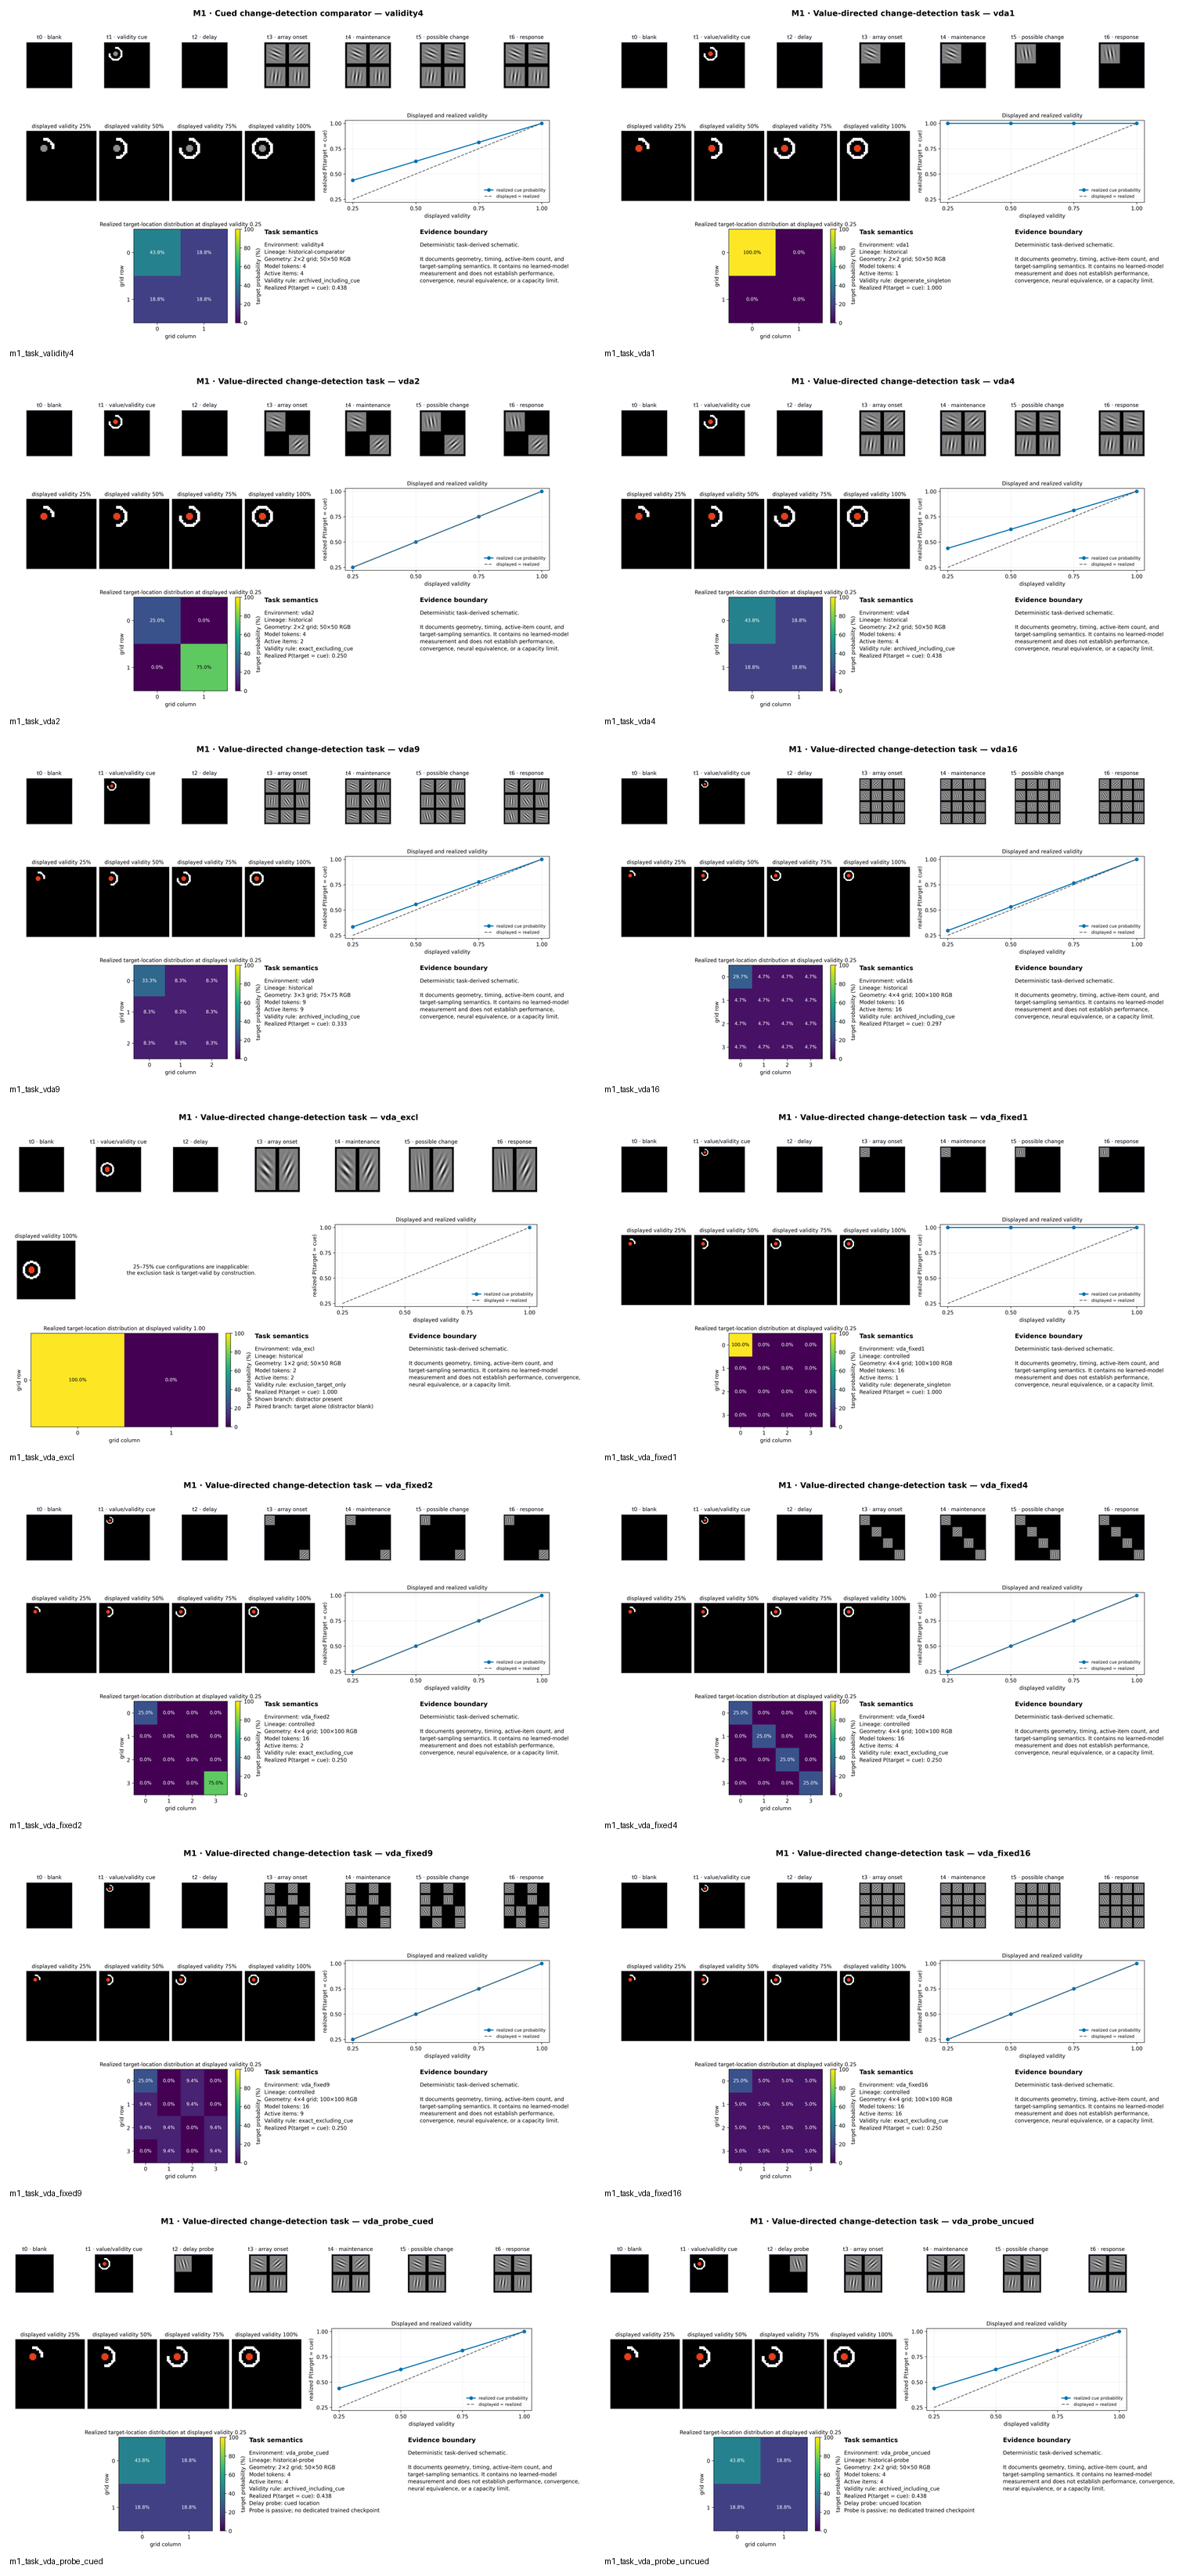
\includegraphics[height=0.68\textheight]{m1_task_contact_sheet.png}
\captionof{figure}{\textbf{M1 task atlas.} \eclass{Deterministic task-derived schematics.} Reading left-to-right and top-to-bottom, tiles show the neutral-validity comparator; historical VDA1/2/4/9/16; the exclusion task; cued and uncued delay probes; and controlled fixed-grid VDA1/2/4/9/16. Every tile uses the same seven-frame sequence, geometry/active-item display, realized-target heatmap, and task-semantics block; cue and change markers retain common encodings. Individual vector products provide full-resolution labels and evidence boundaries.}\label{fig:m1-atlas}
\end{center}\end{landscape}

\MThreeFullPlates

\begin{landscape}
\section{Coverage counts by source object}\label{app:coverage-counts}
\begin{center}
\captionof{table}{\textbf{Overall publication-coverage status.} Counts are panel--environment cells, not independent experiments.}\label{tab:coverage-status}
\begin{tabular}{@{}lrr@{}}
\toprule
Status & Cells & Share \\
\midrule
Complete & 118 & 12.4\% \\
Partial & 79 & 8.3\% \\
Available & 149 & 15.7\% \\
Training & 45 & 4.7\% \\
Blocked & 204 & 21.4\% \\
Undefined & 71 & 7.5\% \\
Inapplicable & 286 & 30.0\% \\
\midrule
Total & 952 & 100.0\% \\
\bottomrule
\end{tabular}

\end{center}
\begingroup
\normalsize
\renewcommand{\arraystretch}{1.10}
\begin{longtable}{@{}lrrrrrrrr@{}}
\caption{Coverage counts by source object. Counts are panel--environment cells, not independent experiments. Status codes are C complete, P partial, A available, T training, B blocked, U undefined, and I inapplicable.}\label{tab:object-counts}\\
\toprule
Object & Groups & C & P & A & T & B & U & I \\
\midrule\endfirsthead
\toprule Object & Groups & C & P & A & T & B & U & I \\ \midrule\endhead
M1 & 3 & 40 & 0 & 0 & 0 & 0 & 2 & 0 \\
M2 & 4 & 56 & 0 & 0 & 0 & 0 & 0 & 0 \\
M3 & 6 & 20 & 0 & 0 & 6 & 26 & 8 & 24 \\
M4 & 4 & 2 & 14 & 3 & 4 & 18 & 5 & 10 \\
M5 & 6 & 0 & 24 & 0 & 6 & 26 & 4 & 24 \\
S1 & 1 & 0 & 0 & 14 & 0 & 0 & 0 & 0 \\
S2 & 1 & 0 & 0 & 14 & 0 & 0 & 0 & 0 \\
S3 & 1 & 0 & 0 & 14 & 0 & 0 & 0 & 0 \\
S4 & 1 & 0 & 0 & 14 & 0 & 0 & 0 & 0 \\
S5 & 2 & 0 & 0 & 0 & 0 & 0 & 0 & 28 \\
S6 & 2 & 0 & 0 & 0 & 0 & 0 & 0 & 28 \\
S7 & 2 & 0 & 0 & 0 & 0 & 0 & 0 & 28 \\
S8 & 1 & 0 & 2 & 3 & 1 & 5 & 3 & 0 \\
S9 & 1 & 0 & 2 & 0 & 1 & 8 & 3 & 0 \\
S10 & 1 & 0 & 2 & 5 & 1 & 6 & 0 & 0 \\
S11 & 2 & 0 & 4 & 8 & 2 & 11 & 3 & 0 \\
S12 & 1 & 0 & 2 & 5 & 1 & 6 & 0 & 0 \\
S13 & 5 & 0 & 5 & 27 & 5 & 20 & 13 & 0 \\
S14 & 3 & 0 & 3 & 18 & 3 & 18 & 0 & 0 \\
S15 & 9 & 0 & 9 & 18 & 9 & 36 & 18 & 36 \\
S16 & 6 & 0 & 12 & 6 & 6 & 24 & 12 & 24 \\
S17 & 6 & 0 & 0 & 0 & 0 & 0 & 0 & 84 \\
\bottomrule
\end{longtable}
\endgroup

\end{landscape}

\begin{landscape}
\section{Exact panel--environment disposition matrix}
Environment abbreviations are: Val4 (\env{validity4}); H1/H2/H4/H9/H16 (historical VDA set sizes); Excl (\env{vda\_excl}); PC/PU (cued/uncued probes); and F1/F2/F4/F9/F16 (controlled fixed-grid set sizes). Status codes are C complete, P partial, A available, T training, B blocked, U undefined, and I inapplicable. Empty status groups are shown with an em dash.

\begingroup
\footnotesize
\setlength{\tabcolsep}{2.5pt}
\renewcommand{\arraystretch}{1.08}
\begin{longtable}{@{}p{1.8cm}p{3.9cm}p{2.2cm}p{2.2cm}p{2.0cm}p{2.3cm}p{2.35cm}p{2.5cm}@{}}
\caption{Exact source-panel disposition by environment. The table is generated directly from \texttt{PANEL\_COVERAGE.csv}; comma-separated abbreviations name every environment assigned to each state.}\label{tab:panel-matrix}\\
\toprule
Panel & Purpose & C/P & Available & Training & Blocked & Undefined & Inapplicable \\
\midrule
\endfirsthead
\multicolumn{8}{c}{\tablename\ \thetable\ (continued)}\\
\toprule
Panel & Purpose & C/P & Available & Training & Blocked & Undefined & Inapplicable \\
\midrule
\endhead
\midrule \multicolumn{8}{r}{Continued on next page}\\ \endfoot
\bottomrule \endlastfoot
M1a & trial sequence & C: Val4, H1, H2, H4, H9, H16, Excl, PC, PU, F1, F2, F4, F9, F16 & \textemdash & \textemdash & \textemdash & \textemdash & \textemdash \\
M1b & cue/value configurations & C: Val4, H1, H2, H4, H9, H16, Excl, PC, PU, F1, F2, F4, F9, F16 & \textemdash & \textemdash & \textemdash & \textemdash & \textemdash \\
M1c & cued versus opposing change examples & C: Val4, H2, H4, H9, H16, Excl, PC, PU, F2, F4, F9, F16 & \textemdash & \textemdash & \textemdash & H1, F1 & \textemdash \\
\addlinespace[2pt]
M2a & patching and visual features & C: Val4, H1, H2, H4, H9, H16, Excl, PC, PU, F1, F2, F4, F9, F16 & \textemdash & \textemdash & \textemdash & \textemdash & \textemdash \\
M2b & routing/allocation mechanism & C: Val4, H1, H2, H4, H9, H16, Excl, PC, PU, F1, F2, F4, F9, F16 & \textemdash & \textemdash & \textemdash & \textemdash & \textemdash \\
M2c & recurrent memory update & C: Val4, H1, H2, H4, H9, H16, Excl, PC, PU, F1, F2, F4, F9, F16 & \textemdash & \textemdash & \textemdash & \textemdash & \textemdash \\
M2d & actor/critic temporal loop & C: Val4, H1, H2, H4, H9, H16, Excl, PC, PU, F1, F2, F4, F9, F16 & \textemdash & \textemdash & \textemdash & \textemdash & \textemdash \\
\addlinespace[2pt]
M3A & response rate by cue validity & C: H1, H2, H4, H9 & \textemdash & F16 & H16, F1, F2, F4, F9 & \textemdash & Val4, Excl, PC, PU \\
M3D & conditional logical response frame by displayed validity & C: H1, H2, H4, H9 & \textemdash & F16 & H16, F1, F2, F4, F9 & \textemdash & Val4, Excl, PC, PU \\
M3B & change-response probability: cued versus archived uncued, low displayed validity & C: H2, H4, H9 & \textemdash & F16 & H16, F2, F4, F9 & H1, F1 & Val4, Excl, PC, PU \\
M3C & change-response probability: cued versus archived uncued, high displayed validity & C: H2, H4, H9 & \textemdash & F16 & H16, F2, F4, F9 & H1, F1 & Val4, Excl, PC, PU \\
M3E & conditional logical response frame: cued versus archived uncued, low displayed validity & C: H2, H4, H9 & \textemdash & F16 & H16, F2, F4, F9 & H1, F1 & Val4, Excl, PC, PU \\
M3F & conditional logical response frame: cued versus archived uncued, high displayed validity & C: H2, H4, H9 & \textemdash & F16 & H16, F2, F4, F9 & H1, F1 & Val4, Excl, PC, PU \\
\addlinespace[2pt]
M4A & allocation maps by cue validity and time & P: H1, H2, H4, H9 & \textemdash & F16 & H16, F1, F2, F4, F9 & \textemdash & Val4, Excl, PC, PU \\
M4B & S1 allocation at change time for S1 changes & C: H4, H9; P: H1, H2, Excl & Val4 & F16 & H16, F1, F2, F4, F9 & \textemdash & PC, PU \\
M4C & S1 allocation when another location changes & P: H2, H4, H9 & Val4 & F16 & H16, F2, F4, F9 & H1, Excl, F1 & PC, PU \\
M4D & S1/S4 allocation over trial time & P: H2, H4, H9, Excl & Val4 & F16 & H16, F2, F4, F9 & H1, F1 & PC, PU \\
\addlinespace[2pt]
M5A & response rate: natural/target intervention & P: H1, H2, H4, H9 & \textemdash & F16 & H16, F1, F2, F4, F9 & \textemdash & Val4, Excl, PC, PU \\
M5B & response rate: matched-location intervention contrast & P: H1, H2, H4, H9 & \textemdash & F16 & H16, F2, F4, F9 & F1 & Val4, Excl, PC, PU \\
M5C & response rate: competing-location intervention contrast & P: H1, H2, H4, H9 & \textemdash & F16 & H16, F2, F4, F9 & F1 & Val4, Excl, PC, PU \\
M5D & reaction time: natural/target intervention & P: H1, H2, H4, H9 & \textemdash & F16 & H16, F1, F2, F4, F9 & \textemdash & Val4, Excl, PC, PU \\
M5E & reaction time: matched-location intervention contrast & P: H1, H2, H4, H9 & \textemdash & F16 & H16, F2, F4, F9 & F1 & Val4, Excl, PC, PU \\
M5F & reaction time: competing-location intervention contrast & P: H1, H2, H4, H9 & \textemdash & F16 & H16, F2, F4, F9 & F1 & Val4, Excl, PC, PU \\
\addlinespace[2pt]
S1 & high-level recurrent circuit & \textemdash & Val4, H1, H2, H4, H9, H16, Excl, PC, PU, F1, F2, F4, F9, F16 & \textemdash & \textemdash & \textemdash & \textemdash \\
\addlinespace[2pt]
S2 & patch-wise recurrent memory & \textemdash & Val4, H1, H2, H4, H9, H16, Excl, PC, PU, F1, F2, F4, F9, F16 & \textemdash & \textemdash & \textemdash & \textemdash \\
\addlinespace[2pt]
S3 & immediate-input allocation before memory & \textemdash & Val4, H1, H2, H4, H9, H16, Excl, PC, PU, F1, F2, F4, F9, F16 & \textemdash & \textemdash & \textemdash & \textemdash \\
\addlinespace[2pt]
S4 & memory feedback into allocation & \textemdash & Val4, H1, H2, H4, H9, H16, Excl, PC, PU, F1, F2, F4, F9, F16 & \textemdash & \textemdash & \textemdash & \textemdash \\
\addlinespace[2pt]
S5a & memory-token architecture & \textemdash & \textemdash & \textemdash & \textemdash & \textemdash & Val4, H1, H2, H4, H9, H16, Excl, PC, PU, F1, F2, F4, F9, F16 \\
S5b-e & memory-token behavior/allocation battery & \textemdash & \textemdash & \textemdash & \textemdash & \textemdash & Val4, H1, H2, H4, H9, H16, Excl, PC, PU, F1, F2, F4, F9, F16 \\
\addlinespace[2pt]
S6a & additive Q/K/V architecture & \textemdash & \textemdash & \textemdash & \textemdash & \textemdash & Val4, H1, H2, H4, H9, H16, Excl, PC, PU, F1, F2, F4, F9, F16 \\
S6b-e & additive Q/K/V behavior/allocation battery & \textemdash & \textemdash & \textemdash & \textemdash & \textemdash & Val4, H1, H2, H4, H9, H16, Excl, PC, PU, F1, F2, F4, F9, F16 \\
\addlinespace[2pt]
S7a & multiplicative Q/K/V architecture & \textemdash & \textemdash & \textemdash & \textemdash & \textemdash & Val4, H1, H2, H4, H9, H16, Excl, PC, PU, F1, F2, F4, F9, F16 \\
S7b-e & multiplicative Q/K/V behavior/allocation battery & \textemdash & \textemdash & \textemdash & \textemdash & \textemdash & Val4, H1, H2, H4, H9, H16, Excl, PC, PU, F1, F2, F4, F9, F16 \\
\addlinespace[2pt]
S8-all & all-slot change-location decoding, natural/max allocation, t5/t6 & P: H4, H9 & Val4, PC, PU & F16 & H2, H16, F2, F4, F9 & H1, Excl, F1 & \textemdash \\
\addlinespace[2pt]
S9-all & all-slot location decoding across four allocation conditions & P: H4, H9 & \textemdash & F16 & Val4, H2, H16, PC, PU, F2, F4, F9 & H1, Excl, F1 & \textemdash \\
\addlinespace[2pt]
S10-all & single-slot binary change decoding across allocation conditions & P: H4, H9 & Val4, H1, Excl, PC, PU & F16 & H2, H16, F1, F2, F4, F9 & \textemdash & \textemdash \\
\addlinespace[2pt]
S11-location & actor-layer change-location decoding & P: H4, H9 & Val4, PC, PU & F16 & H2, H16, F2, F4, F9 & H1, Excl, F1 & \textemdash \\
S11-binary & actor-layer binary change decoding & P: H4, H9 & Val4, H1, Excl, PC, PU & F16 & H2, H16, F1, F2, F4, F9 & \textemdash & \textemdash \\
\addlinespace[2pt]
S12-all & graded actor-layer binary decoding under S1 inhibition & P: H4, H9 & Val4, H1, Excl, PC, PU & F16 & H2, H16, F1, F2, F4, F9 & \textemdash & \textemdash \\
\addlinespace[2pt]
S13-all & all-trial Wait/Declare logit scatter and density & P: H9 & Val4, H1, H2, H4, Excl, PC, PU & F16 & H16, F1, F2, F4, F9 & \textemdash & \textemdash \\
S13-S1 & Wait/Declare logit scatter and density for S1 changes & P: H9 & Val4, H1, H2, H4, Excl, PC, PU & F16 & H16, F1, F2, F4, F9 & \textemdash & \textemdash \\
S13-S2 & Wait/Declare logit scatter and density for S2 changes & P: H9 & Val4, H2, H4, PC, PU & F16 & H16, F2, F4, F9 & H1, Excl, F1 & \textemdash \\
S13-S3 & Wait/Declare logit scatter and density for S3 changes & P: H9 & Val4, H4, PC, PU & F16 & H16, F4, F9 & H1, H2, Excl, F1, F2 & \textemdash \\
S13-S4 & Wait/Declare logit scatter and density for S4 changes & P: H9 & Val4, H4, PC, PU & F16 & H16, F4, F9 & H1, H2, Excl, F1, F2 & \textemdash \\
\addlinespace[2pt]
S14-natural & natural S1-change logit scatter/density & P: H9 & Val4, H1, H4, Excl, PC, PU & F16 & H2, H16, F1, F2, F4, F9 & \textemdash & \textemdash \\
S14-max & maximal S1 allocation logit scatter/density & P: H9 & Val4, H1, H4, Excl, PC, PU & F16 & H2, H16, F1, F2, F4, F9 & \textemdash & \textemdash \\
S14-zero & zero S1 allocation logit scatter/density & P: H9 & Val4, H1, H4, Excl, PC, PU & F16 & H2, H16, F1, F2, F4, F9 & \textemdash & \textemdash \\
\addlinespace[2pt]
S15A & TD error by cue/change location & P: H9 & H2, H4 & F16 & H16, F2, F4, F9 & H1, F1 & Val4, Excl, PC, PU \\
S15B & TD error with target allocation clamp, low cue & P: H9 & H2, H4 & F16 & H16, F2, F4, F9 & H1, F1 & Val4, Excl, PC, PU \\
S15C & TD error with target allocation clamp, high cue & P: H9 & H2, H4 & F16 & H16, F2, F4, F9 & H1, F1 & Val4, Excl, PC, PU \\
S15D & TD error by allocation dose and location & P: H9 & H2, H4 & F16 & H16, F2, F4, F9 & H1, F1 & Val4, Excl, PC, PU \\
S15E & TD error under competing-location clamp, low cue & P: H9 & H2, H4 & F16 & H16, F2, F4, F9 & H1, F1 & Val4, Excl, PC, PU \\
S15F & TD error under competing-location clamp, high cue & P: H9 & H2, H4 & F16 & H16, F2, F4, F9 & H1, F1 & Val4, Excl, PC, PU \\
S15G & value by change magnitude with target clamp & P: H9 & H2, H4 & F16 & H16, F2, F4, F9 & H1, F1 & Val4, Excl, PC, PU \\
S15H & value by opposing-location allocation dose & P: H9 & H2, H4 & F16 & H16, F2, F4, F9 & H1, F1 & Val4, Excl, PC, PU \\
S15I & hit rate by opposing-location allocation dose & P: H9 & H2, H4 & F16 & H16, F2, F4, F9 & H1, F1 & Val4, Excl, PC, PU \\
\addlinespace[2pt]
S16A & criterion vs allocation at change & P: H4, H9 & H2 & F16 & H16, F2, F4, F9 & H1, F1 & Val4, Excl, PC, PU \\
S16B & criterion vs cue-time allocation with change-time control & P: H4, H9 & H2 & F16 & H16, F2, F4, F9 & H1, F1 & Val4, Excl, PC, PU \\
S16C & criterion vs cue-time allocation & P: H4, H9 & H2 & F16 & H16, F2, F4, F9 & H1, F1 & Val4, Excl, PC, PU \\
S16D & sensitivity vs allocation at change & P: H4, H9 & H2 & F16 & H16, F2, F4, F9 & H1, F1 & Val4, Excl, PC, PU \\
S16E & sensitivity vs cue-time allocation with change-time control & P: H4, H9 & H2 & F16 & H16, F2, F4, F9 & H1, F1 & Val4, Excl, PC, PU \\
S16F & sensitivity vs cue-time allocation & P: H4, H9 & H2 & F16 & H16, F2, F4, F9 & H1, F1 & Val4, Excl, PC, PU \\
\addlinespace[2pt]
S17-action-behavior & three behavioral rows: supervised actions & \textemdash & \textemdash & \textemdash & \textemdash & \textemdash & Val4, H1, H2, H4, H9, H16, Excl, PC, PU, F1, F2, F4, F9, F16 \\
S17-belief-behavior & three behavioral rows: supervised beliefs & \textemdash & \textemdash & \textemdash & \textemdash & \textemdash & Val4, H1, H2, H4, H9, H16, Excl, PC, PU, F1, F2, F4, F9, F16 \\
S17-rl-behavior & three behavioral rows: reinforcement learning & \textemdash & \textemdash & \textemdash & \textemdash & \textemdash & Val4, H1, H2, H4, H9, H16, Excl, PC, PU, F1, F2, F4, F9, F16 \\
S17-action-allocation & allocation row: supervised actions & \textemdash & \textemdash & \textemdash & \textemdash & \textemdash & Val4, H1, H2, H4, H9, H16, Excl, PC, PU, F1, F2, F4, F9, F16 \\
S17-belief-allocation & allocation row: supervised beliefs & \textemdash & \textemdash & \textemdash & \textemdash & \textemdash & Val4, H1, H2, H4, H9, H16, Excl, PC, PU, F1, F2, F4, F9, F16 \\
S17-rl-allocation & allocation row: reinforcement learning & \textemdash & \textemdash & \textemdash & \textemdash & \textemdash & Val4, H1, H2, H4, H9, H16, Excl, PC, PU, F1, F2, F4, F9, F16 \\
\end{longtable}
\endgroup

\end{landscape}

\begin{landscape}
\section{Matched-width constituent values}\label{app:matched-width-constituents}
The tables expose the absolute and within-checkpoint values behind the d256-minus-d128 summary. They are regenerated by \path{reports/vda_series/manuscript/build_constituent_tables.py}, which verifies all twelve shard hashes against the immutable upstream manifest before reading arrays; the machine-readable companion is \path{generated/matched_width_constituents.json}.
\begingroup\scriptsize\setlength{\tabcolsep}{2.7pt}
\captionof{table}{\textbf{Absolute valid-location response probabilities.} Checkpoint-recomputed values at displayed validity 0.75; each cell uses 300 trials. These are the constituents behind Figure~\ref{fig:matched-width}A, not replicated estimates of a width effect.}\label{tab:absolute-behavior}
\begin{center}
\begin{tabular}{@{}llr*{10}{r}@{}}
\toprule
Task & Routing & Width & \multicolumn{10}{c}{Orientation change (degrees)} \\
\cmidrule(lr){4-13}
 & & & 2 & 6 & 10 & 14 & 18 & 22 & 26 & 30 & 34 & 38 \\ 
\midrule
VDA1 & \texttt{affine} & 128 & 0.133 & 0.250 & 0.460 & 0.697 & 0.903 & 0.923 & 0.960 & 0.957 & 0.953 & 0.947 \\
VDA1 & \texttt{affine} & 256 & 0.123 & 0.230 & 0.487 & 0.653 & 0.907 & 0.917 & 0.953 & 0.953 & 0.947 & 0.963 \\
VDA1 & \texttt{cross-attn} & 128 & 0.060 & 0.123 & 0.313 & 0.520 & 0.717 & 0.843 & 0.863 & 0.873 & 0.890 & 0.857 \\
VDA1 & \texttt{cross-attn} & 256 & 0.177 & 0.287 & 0.480 & 0.730 & 0.810 & 0.910 & 0.897 & 0.907 & 0.923 & 0.897 \\
VDA4 & \texttt{affine} & 128 & 0.093 & 0.177 & 0.437 & 0.663 & 0.833 & 0.947 & 0.973 & 0.997 & 1.000 & 1.000 \\
VDA4 & \texttt{affine} & 256 & 0.120 & 0.337 & 0.587 & 0.777 & 0.933 & 0.980 & 0.990 & 0.997 & 0.997 & 1.000 \\
VDA4 & \texttt{cross-attn} & 128 & 0.063 & 0.140 & 0.410 & 0.617 & 0.803 & 0.967 & 0.980 & 1.000 & 1.000 & 1.000 \\
VDA4 & \texttt{cross-attn} & 256 & 0.037 & 0.113 & 0.303 & 0.487 & 0.690 & 0.923 & 0.953 & 0.993 & 1.000 & 1.000 \\
VDA9 & \texttt{affine} & 128 & 0.073 & 0.170 & 0.420 & 0.640 & 0.863 & 0.970 & 0.990 & 1.000 & 1.000 & 1.000 \\
VDA9 & \texttt{affine} & 256 & 0.087 & 0.140 & 0.407 & 0.597 & 0.813 & 0.963 & 0.983 & 0.997 & 1.000 & 1.000 \\
\bottomrule
\end{tabular}
\end{center}
\endgroup

\begingroup\scriptsize\setlength{\tabcolsep}{4.0pt}
\captionof{table}{\textbf{Within-checkpoint clamp constituents.} Each entry is $D_{w,x}(b)=d'_{w,x}(b)-d'_{w,x}(0)$ from 250 trials per bias, condition, and checkpoint. VDA1 invalid-location effects are undefined and therefore absent. Figure~\ref{fig:matched-width}C--D plots $W_x(b)=D_{256,x}(b)-D_{128,x}(b)$.}\label{tab:clamp-constituents}
\begin{center}
\begin{tabular}{@{}llll*{5}{r}@{}}
\toprule
Task & Routing & Condition & Width & \multicolumn{5}{c}{Assigned key-logit bias $b$} \\
\cmidrule(lr){5-9}
 & & & & -6 & -3 & 0 & 3 & 6 \\ 
\midrule
VDA1 & \texttt{affine} & valid & 128 & -1.681 & -1.124 & 0.000 & -0.474 & -0.572 \\
VDA1 & \texttt{affine} & valid & 256 & -0.017 & -0.017 & 0.000 & -0.017 & -0.020 \\
VDA1 & \texttt{cross-attn} & valid & 128 & -0.470 & 0.054 & 0.000 & 0.071 & 0.137 \\
VDA1 & \texttt{cross-attn} & valid & 256 & 0.087 & 0.028 & 0.000 & -0.019 & -0.102 \\
VDA4 & \texttt{affine} & valid & 128 & -1.384 & -0.622 & 0.000 & 0.247 & 0.092 \\
VDA4 & \texttt{affine} & invalid & 128 & 0.375 & 0.351 & 0.000 & -0.785 & -1.484 \\
VDA4 & \texttt{affine} & valid & 256 & -0.491 & -0.176 & 0.000 & 0.046 & -0.156 \\
VDA4 & \texttt{affine} & invalid & 256 & 0.284 & 0.146 & 0.000 & -0.377 & -0.787 \\
VDA4 & \texttt{cross-attn} & valid & 128 & -0.544 & -0.426 & 0.000 & -0.297 & -0.456 \\
VDA4 & \texttt{cross-attn} & invalid & 128 & 0.172 & 0.172 & 0.000 & -0.610 & -0.750 \\
VDA4 & \texttt{cross-attn} & valid & 256 & -0.736 & -0.577 & 0.000 & -0.009 & -0.047 \\
VDA4 & \texttt{cross-attn} & invalid & 256 & 0.117 & 0.133 & 0.000 & -0.434 & -0.574 \\
VDA9 & \texttt{affine} & valid & 128 & -0.978 & -0.300 & 0.000 & -0.097 & -0.199 \\
VDA9 & \texttt{affine} & invalid & 128 & 0.420 & 0.391 & 0.000 & -0.187 & -0.462 \\
VDA9 & \texttt{affine} & valid & 256 & -0.046 & 0.040 & 0.000 & 0.086 & 0.097 \\
VDA9 & \texttt{affine} & invalid & 256 & 0.150 & 0.076 & 0.000 & -0.160 & -0.378 \\
\bottomrule
\end{tabular}
\end{center}
\endgroup

\end{landscape}

\section{Artifact locations and provenance classes}
\begin{tabularx}{\textwidth}{@{}p{3.2cm}Y Y@{}}
\toprule
Artifact & Path & Provenance class\\
\midrule
This manuscript & \path{reports/vda_series/manuscript/main.pdf} & Newly authored and compiled on 12 July 2026\\
M1 task products & \path{reports/vda_series/figures/task/} & Newly regenerated deterministic specifications\\
M2 architecture & \path{reports/vda_series/figures/architecture/} & Newly authored source-derived specification diagrams\\
M3 behavior & \path{reports/vda_series/figures/behavior/} & Newly regenerated plots from preserved aggregate NPZ\\
First-wave checkpoint products & \path{reports/vda_series/figures/first_wave/} & Byte-identical publication snapshots from the independently approved 96/300 production build\\
First-wave production QA & \path{RViT_plus_paper_jepa_grid9/reports/vda_series/first_wave_20260711_production_QA.md} & Dated semantic, provenance, format, and visual approval record\\
Matched-width publication snapshots & \path{reports/vda_series/figures/matched_width/} & Locally manifested PDF/SVG/PNG/JSON and production-manifest projection from the audited v15 summary\\
Matched-width production root & \path{reports/vda_series/matched_width_20260712_production_v15/} & Exact-inventory summary bound to the immutable 12-file upstream battery\\
Panel inventory & \path{reports/vda_series/MAH_SOURCE_PANEL_INVENTORY.md} & Newly authored source-grounded inventory\\
Coverage matrix & \path{reports/vda_series/PANEL_COVERAGE.csv} & Newly authored machine-readable disposition matrix\\
Older upgraded manuscript & \path{reports/upgraded_paper/manuscript/main.pdf} & Rebuilt from an older manuscript lineage; not this report\\
Preserved VDA9 reports & historical report directories & Preserved older artifacts; visually audited, not relabeled as new\\
\bottomrule
\end{tabularx}

\clearpage
\begin{thebibliography}{9}
\bibitem{mah2025} J. Morgan, L. Albanna, and J. P. Herman. \emph{Recurrent vision transformers model visual attention through feedback}. arXiv:2502.10955v1, 2025.

\bibitem{carrasco2011} M. Carrasco. Visual attention: the past 25 years. \emph{Vision Research}, 2011. doi:10.1016/j.visres.2011.04.012.

\bibitem{herman2017} J. P. Herman and R. J. Krauzlis. Color-change detection activity in the primate superior colliculus. \emph{eNeuro}, 2017. doi:10.1523/ENEURO.0046-17.2017.

\bibitem{luo2018} T. Z. Luo and J. H. R. Maunsell. Attentional changes in either criterion or sensitivity are associated with robust modulations in lateral prefrontal cortex. \emph{Neuron}, 2018. doi:10.1016/j.neuron.2018.02.007.

\bibitem{moore2003} T. Moore and K. M. Armstrong. Selective gating of visual signals by microstimulation of frontal cortex. \emph{Nature}, 2003. doi:10.1038/nature01341.

\bibitem{luck1997} S. J. Luck and E. K. Vogel. The capacity of visual working memory for features and conjunctions. \emph{Nature}, 1997. doi:10.1038/36846.

\bibitem{panichello2021} M. F. Panichello and T. J. Buschman. Shared mechanisms underlie the control of working memory and attention. \emph{Nature}, 2021. doi:10.1038/s41586-021-03390-w.
\end{thebibliography}

\end{document}
